\documentclass[a4paper, fontsize = 8pt, landscape]{scrartcl}
\usepackage{../../../misc_files/LateX/layout_and_colours}
\makeatletter
\def\input@path{{content/exam_summary/}{content/examples/}}
\makeatother
\graphicspath{{content/images/}{content/exam_summary/images/}{content/examples/images/}}

\title{Höhere Mathematik 2}
\author{Jil Zerndt}
\date{FS 2025}

\createtitlepagestyle
\createmainpagestyle
\begin{document}
\begin{multicols}{3}
	\thispagestyle{TitlePageStyle}
	\maketitle
	\sffamily
	\section{Numerische Lösung nicht linearer Gleichungssysteme}

\begin{remark}
    LGS = lineares Gleichungssystem, NGS = nichtlineares Gleichungssystem
\end{remark}



\raggedcolumns

\begin{definition}{Skalarwertige Funktionen}
    $f: D \subset \R^n \to W \subset \R$
    \vspace{-2mm}
    $$(x_1, x_2, \ldots, x_n) \mapsto y = f(x_1, x_2, \ldots, x_n)$$
    \small
    $f$ mit $n$ unabhängigen Variablen $x_1, \ldots, x_n$ und einer abhängigen Variablen $y$,
    die jedem $(x_1, x_2, \ldots, x_n)$ aus Definitionsmenge $D \subset \R^n$ genau ein $y \in W \subset \R$ zuordnet.
    Ergebnis: $y \in \R$ = Skalar (eine Zahl) 
\end{definition}

\begin{concept}{Vektorwertige Funktion} gibt einen \textbf{Vektor} zurück (statt Skalar)\\
    Sei $\textbf{f}: \R^n \to \R^m$ eine Funktion mit $n$ Variablen.
    \vspace{-2mm}
    $$\textbf{f}(x_1 \ldots, x_n) = \begin{psmallmatrix} y_1 = f_1(x_1, x_2, \ldots, x_n) \\ y_2 = f_2(x_1, x_2, \ldots, x_n) \\ ... \\ y_m = f_m(x_1, x_2, \ldots, x_n) \end{psmallmatrix}$$
    \small wobei die $m$ Komponenten $f_i: \R^n \to \R$ für $i = 1, 2, \ldots, n$ von $\textbf{f}$ wieder \textbf{skalarwertige} Funktionen sind.
\end{concept}

\begin{theorem}{Nichtlineares Gleichungssystem (NGS)}\\
    Lösungen des NGS sind Nullstellen der Funktion:
    \vspace{-2mm}
    $$\textbf{f}: \R^2 \to \R^2 \quad \textbf{f}(x) = \begin{psmallmatrix} f_1 (x_1, x_2) \\ f_2 (x_1, x_2) \end{psmallmatrix} = \begin{psmallmatrix} 0\\ 0 \end{psmallmatrix}$$
    \small
    Ein solches System lässt sich nicht in die Form $Ax = b$ bringen. \\
    Geometrisch lassen sich die Lösungen als Schnittpunkte der beiden Funktionen interpretieren.
\end{theorem}

\begin{corollary}{Lineare Funktionen von LGS}
    $$\textbf{A} \overrightarrow{\textbf{x}} = \overrightarrow{\textbf{b}} \Rightarrow \underbrace{\textbf{A} \overrightarrow{\textbf{x}} - \overrightarrow{\textbf{b}} = \overrightarrow{\textbf{0}}}_{\overrightarrow{\textbf{f}}(\overrightarrow{\textbf{x}})} \Rightarrow \overrightarrow{\textbf{f}}(x_1, x_2, x_3) = 0 \begin{psmallmatrix} x_1 \\ x_2 \\ x_3 \end{psmallmatrix} = \begin{psmallmatrix} 0 \\ 0 \\ 0 \end{psmallmatrix}$$
    \resizebox{\textwidth}{!}{
    $\overrightarrow{\textbf{f}}(\overrightarrow{\textbf{x}}) = \textbf{A} \overrightarrow{\textbf{x}} - \overrightarrow{\textbf{b}} = \begin{psmallmatrix} 4 & -1 & 1 \\ -2 & 5 & 1 \\ 1 & -2 & 5 \end{psmallmatrix} \begin{psmallmatrix} x_1 \\ x_2 \\ x_3 \end{psmallmatrix} - \begin{psmallmatrix} 5 \\ 11 \\ 12 \end{psmallmatrix}, \quad
    \textbf{f}(x_1, x_2, x_3) = \begin{psmallmatrix} f_1 = 4x_1 - x_2 + x_3 - 5 \\ f_2 = -2x_1 + 5x_2 + x_3 - 11 \\ f_3 = x_1 - 2x_2 + 5x_3 - 12 \end{psmallmatrix}$}
\end{corollary}


\begin{concept}{Analytische Darstellung}
    \begin{itemize}
        \item \textbf{Explizite Darstellung:} $y = f(x_1, \ldots, x_n)$
        \item \textbf{Implizite Darstellung:} $F(x, y) = 0$
        \item \textbf{Parameterdarstellung:} $x = x(t), y = y(t)$
    \end{itemize}
\end{concept}

\begin{concept}{Darstellung durch Wertetabelle}
    Sei $f: \R^n \to \R^m$ eine Funktion.\\
    In $z = f(x,y)$ Werte von $x$ und $y$ einsetzen (der Reihe nach): \\
    $$\begin{psmallmatrix} z_{11} & z_{12} & \ldots & z_{1m} \\ z_{m1} & z_{m2} & \ldots & z_{mn} \end{psmallmatrix} \quad\quad\quad\quad\quad\quad\quad\quad\quad\quad\quad\quad\quad\quad.$$
\end{concept}

\begin{minipage}{0.5\linewidth}
\begin{concept}{Funktion als Fläche im Raum}\\
    $f$ ordnet jedem Punkt $(x, y) \in D$ in Ebene Wert $z=f(x, y)$ zu \\($\rightarrow$ Höhenkoordinate)    
\end{concept}

\begin{concept}{Schnittkurvendiagramm}\\
    Fläche $z=f(x, y)$ bei konstanten Höhe $z$ schneiden: Schnittkurve. 
    Diese in $(x, y)$-Ebene projizieren: Höhenlinie.
\end{concept}
\end{minipage}
\begin{minipage}{0.5\linewidth}
\vspace{-8mm}
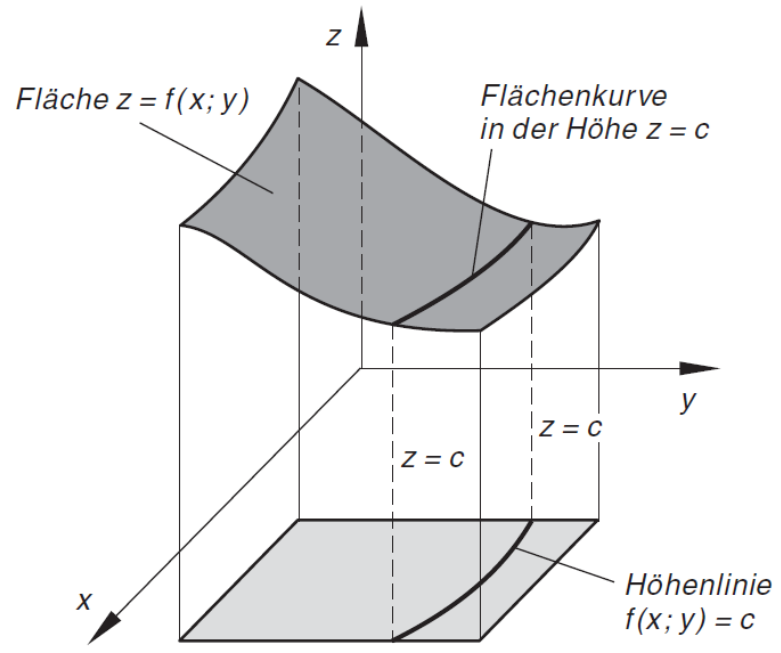
\includegraphics[width=\linewidth]{grafische_darstellung_detailed.png}
\small hellgraue Fläche = Definitionsbereich D
\end{minipage}

\subsubsection{Partielle Ableitungen}

\begin{theorem}{Partielle Ableitung}
$
f^{\prime}(x_0)=\lim _{\Delta x \rightarrow 0} \frac{(f(x_0+\Delta x)-f(x_0))}{\Delta x}
$
$$\text{Ableitung nach x: } f_x=\frac{\partial f}{\partial x}(x, y)=\lim _{\Delta x \rightarrow 0} \frac{f(x+\Delta x, y)-f(x, y)}{\Delta x}$$
$$\text{Ableitung nach y: } f_y=\frac{\partial f}{\partial y}(x, y)=\lim _{\Delta y \rightarrow 0} \frac{f(x, y+\Delta y)-f(x, y)}{\Delta y}$$
\end{theorem}



\begin{KR}{Partielle Ableitungen berechnen}
    \small
    \begin{enumerate}
        \item Variable identifizieren: nach welcher Variable ableiten?
        \item Alle anderen Variablen während Ableitung nur Konstanten
        \item Standardableitungsregeln anwenden und Ergebnis korrekt notieren
    \end{enumerate}
\end{KR}

\begin{definition}{Jacobi-Matrix}
    \resizebox{0.7\textwidth}{!}{
$f: \mathbb{R}^n \rightarrow \mathbb{R}^m$ mit $y = f(x)$ und $x = (x_1, x_2, ..., x_n)^T \in \mathbb{R}^n$}

Jacobi-Matrix enthält alle partiellen Ableitungen 1. Ordnung von $f$:
\vspace{-2mm}\\
$$f(x) = \begin{psmallmatrix}
    y_1=f_1(x) \\
    y_2=f_2(x) \\
    ...\\
    y_m=f_m(x)
\end{psmallmatrix} \rightarrow 
Df(x) := \begin{bsmallmatrix}
\frac{\partial f_1}{\partial x_1}(x) & \frac{\partial f_1}{\partial x_2}(x) & \cdots & \frac{\partial f_1}{\partial x_n}(x) \\
\frac{\partial f_2}{\partial x_1}(x) & \frac{\partial f_2}{\partial x_2}(x) & \cdots & \frac{\partial f_2}{\partial x_n}(x) \\
\cdots & \cdots & \cdots & \cdots \\
\frac{\partial f_m}{\partial x_1}(x) & \frac{\partial f_m}{\partial x_2}(x) & \cdots & \frac{\partial f_m}{\partial x_n}(x)
\end{bsmallmatrix}$$
\end{definition}

\begin{concept}{Linearisierung}
Die verallgemeinerte \textcolor{purple}{\textbf{Tangentengleichung}}
$$g(x) = f(x^{(0)}) + Df(x^{(0)}) \cdot (x - x^{(0)})$$ 
\small
beschreibt lineare Funktion, $f(x) \approx g(x)$ in Umgebung von $x^{(0)}=(x_1^{(0)}, x_2^{(0)}, \ldots, x_n^{(0)})^T \in \mathbb{R}^n$. 
Man spricht von der \textbf{Linearisierung} der Funktion $y = f(x)$ in einer Umgebung von $x^{(0)}$ ($x^{(k)}$ bezeichnet Vektor aus $\R^n$ nach $k$-ter Iteration).
\end{concept}

\begin{corollary}{Tangentialebene}
    \resizebox{0.7\textwidth}{!}{
    $f: \mathbb{R}^2 \longrightarrow \mathbb{R}$, $y=f(x_1, x_2)$, $\boldsymbol{x}^{(0)}=(x_1^{(0)}, x_2^{(0)})^T \in \mathbb{R}^2$ }

    Spezielle Jacobi-Matrix (nur ein Zeilenvektor mit zwei Elementen):
    \vspace{-2mm}\\
    $$Df(x^{(0)}) = \left(\frac{\partial f}{\partial x_1}(x_1^{(0)}, x_2^{(0)}), \frac{\partial f}{\partial x_2}(x_1^{(0)}, x_2^{(0)})\right)$$
    Linearisierung $g(x_1, x_2)$ die Gleichung der Tangentialebene: 
    $$=f(x_1^{(0)}, x_2^{(0)}) + (\frac{\partial f}{\partial x_1}(x_1^{(0)}, x_2^{(0)}), \frac{\partial f}{\partial x_2}(x_1^{(0)}, x_2^{(0)})) \cdot \binom{x_1 - x_1^{(0)}}{x_2 - x_2^{(0)}}$$
    $$= f(x_1^{(0)}, x_2^{(0)}) + \frac{\partial f}{\partial x_1}(x_1^{(0)}, x_2^{(0)}) \cdot (x_1 - x_1^{(0)}) + \frac{\partial f}{\partial x_2}(x_1^{(0)}, x_2^{(0)}) \cdot (x_2 - x_2^{(0)})$$
    \small
    Sie enthält sämtliche im Flächenpunkt 
    $\stackrel{\bullet}{P}=(x_1^{(0)}, x_2^{(0)}, f(x_1^{(0)}, x_2^{(0)}))$ \\
    an die Bildfläche von $y=f(x_1, x_2)$ angelegten Tangenten.
\end{corollary}

\begin{KR}{Jacobi-Matrix berechnen und linearisieren}\\
Sei $f: \mathbb{R}^n \rightarrow \mathbb{R}^m$ mit $y = f(x)$ und $x = (x_1, x_2, ..., x_n)^T \in \mathbb{R}^n$. 
\vspace{-2mm}\\
\begin{enumerate}
    \item Identifiziere die Komponentenfunktionen $f_1, f_2, ..., f_m$ und \\ Variablen $x_1, x_2, ..., x_n$.
    \item Berechne partielle Ableitungen $\frac{\partial f_i}{\partial x_j}$ für $i = 1, ..., m$, $j = 1, ..., n$.
    \item Stelle die Jacobi-Matrix $Df(x)$ auf
    \item Werte Jacobi-Matrix an Entwicklungspunkt $x^{(0)}$ aus\\ (Werte für $x_1, x_2, ..., x_n$ einsetzen)
    \item Berechne Linearisierung $g(x)$ mit Tangentengleichung
\end{enumerate}
\end{KR}

\begin{remark}
    Struggle $\in \R$
\end{remark}

\begin{example2}{Jacobi-Matrix und Linearisierung} \small
$f(x, y, z) = \begin{psmallmatrix} e^{xy} + z^2 - 3 \\ \sin(x + y) - z \\ x^2 + y^2 + z^2 - 6 \end{psmallmatrix}$

\textbf{Jacobi-Matrix:}
$Df(x, y, z) = \begin{bsmallmatrix} ye^{xy} & xe^{xy} & 2z \\ \cos(x + y) & \cos(x + y) & -1 \\ 2x & 2y & 2z \end{bsmallmatrix}$

\textbf{Linearisierung an $(1, 0, 1)^T$:}

\resizebox{\textwidth}{!}{
$f(1, 0, 1) = \begin{psmallmatrix} e^0 + 1 - 3 \\ \sin(1) - 1 \\ 1 + 0 + 1 - 6 \end{psmallmatrix} = \begin{psmallmatrix} -1 \\ \sin(1) - 1 \\ -4 \end{psmallmatrix}, \quad
Df(1, 0, 1) = \begin{bsmallmatrix} 0 & 1 & 2 \\ \cos(1) & \cos(1) & -1 \\ 2 & 0 & 2 \end{bsmallmatrix}$}

Linearisierung: $g(x, y, z) = f(1, 0, 1) + Df(1, 0, 1) \cdot \begin{psmallmatrix} x - 1 \\ y - 0 \\ z - 1 \end{psmallmatrix}$

$$g(x, y, z) = \begin{psmallmatrix} -1 + y + 2(z-1) \\ \sin(1) - 1 + \cos(1)(x-1) + \cos(1)y - (z-1) \\ -4 + 2(x-1) + 2(z-1) \end{psmallmatrix}$$

\textbf{Geometrische Bedeutung:}
Linearisierung approximiert nichtlineare Funktion $f$ nahe des Punktes $(1, 0, 1)^T$ durch lineare Funktion. Entspricht der Tangentialebene an die durch $f = 0$ definierte Fläche im 3D Raum.
\end{example2}

\raggedcolumns

\subsubsection{Nullstellenbestimmung für NGS}

\begin{definition}{Problemstellung zur Nullstellenbestimmung}\\
Gegeben: $n \in \mathbb{N}$, $f: \mathbb{R}^n \rightarrow \mathbb{R}^n$ Gesucht: Vektor $\bar{x} \in \mathbb{R}^n$ mit $f(\bar{x}) = 0$

Komponentenweise: Gegeben: $n$ Funktionen $f_i: \mathbb{R}^n \rightarrow \mathbb{R}$ (Komponenten von $f$) Gesucht: Vektor $\bar{x} \in \mathbb{R}^n$ mit $f_i(\bar{x}) = 0$ für $i = 1, ..., n$.
\end{definition}

\begin{KR}{Newton-Verfahren für NGS} \small{(Quadratische Konv.)}\\
    \normalsize
    Gesucht: Nullstellen von $f: \mathbb{R}^n \rightarrow \mathbb{R}^n$
    
    $x^{(0)}$ = Startvektor nahe einer Nullstelle

    \textbf{Vorbereitung}: definiere $f(x) = 0$, berechne $Df(x)$, wähle $x^{(0)}$

    \textbf{Für jede Iteration $n$}:
    \begin{enumerate}
        \item Linearisierung um $x^{n}$: Berechne $f(x^{(n)})$ und $D f(x^{(n)})$
        \item Nullstellen der Linearisierung: $\delta^{(n)}$ als Lösung des LGS\\
        $Df(x^{(n)}) \cdot \delta^{(n)} = -f(x^{(n)})$
        \item Setze $x^{(n+1)} := x^{(n)} + \delta^{(n)}$ (nächste Iteration)
        \item \small Weiterführen bis: $\|f(x^{(n+1)})\|_2 < \text{TOL}$ oder $\|x^{(n+1)} - x^{(n)}\|_2 < \text{TOL}$.
    \end{enumerate}
    \small
    \textbf{Interpretation:} Konvergierte Lösung $x^{(n)}$ = Näherung für Nullstelle von $f$
\end{KR}

\begin{theorem}{Vereinfachtes Newton-Verfahren} (Lineare Konvergenz)

    Lösung von $f(x)=0$ mit $f: \mathbb{R}^n \rightarrow \mathbb{R}^n$ für $n=0,1,2, \ldots$
    \begin{enumerate}
        \item Berechne $f(x^{(n)})$ und $D f(x^{(0)})$
        \item Berechne $\delta^{(n)}$ als Lösung des LGS $D f(x^{(0)}) \cdot \delta^{(n)}=-f(x^{(n)})$
        \item Setze $x^{(n+1)}:=x^{(n)}+\delta^{(n)}$
        \item \small Weiterführen bis: $\|f(x^{(n+1)})\|_2 < \text{TOL}$ oder $\|x^{(n+1)} - x^{(n)}\|_2 < \text{TOL}$.
    \end{enumerate}
\end{theorem}

\begin{corollary}{Fehler-Normen}
    \begin{itemize}
        \item $\|f(x)\|_2 = \sqrt{\sum_{i=1}^n f_i(x)^2}$: Euklidische Norm
        \item $\|x\|_2 = \sqrt{x_1^2 + x_2^2 + ... + x_n^2}$: Euklidische Norm für Vektoren
        \item $\|A\|_2 = \max_{\|x\|_2=1} \|Ax\|_2$: Operatornorm für Matrizen
    \end{itemize}
\end{corollary}

\begin{example2}{Newton-Verfahren} \small
$f(x_1, x_2) = \begin{psmallmatrix} 20 - 18x_1 - 2x_2^2 \\ -4x_2(x_1 - x_2^2) \end{psmallmatrix}$, $x^{(0)} = (1.1, 0.9)^T$

\textbf{Jacobi-Matrix:} 
$Df(x_1, x_2) = \begin{bsmallmatrix} -18 & -4x_2 \\ -4x_2 & -4(x_1 - 3x_2^2) \end{bsmallmatrix}$

\textbf{Erste Iteration:}  ($k = 0$)
$f(1.1, 0.9) = \begin{psmallmatrix} -1.42 \\ -0.036 \end{psmallmatrix}$

$Df(1.1, 0.9) = \begin{bsmallmatrix} -18 & -3.6 \\ -3.6 & -5.32 \end{bsmallmatrix}$

LGS lösen: $\begin{bsmallmatrix} -18 & -3.6 \\ -3.6 & -5.32 \end{bsmallmatrix} \delta^{(0)} = \begin{psmallmatrix} 1.42 \\ 0.036 \end{psmallmatrix}$
$\Rightarrow \delta^{(0)} = \begin{psmallmatrix} -0.0822 \\ 0.0178 \end{psmallmatrix}$
$$x^{(1)} = \begin{psmallmatrix} 1.1 \\ 0.9 \end{psmallmatrix} + \begin{psmallmatrix} -0.0822 \\ 0.0178 \end{psmallmatrix} = \begin{psmallmatrix} 1.0178 \\ 0.9178 \end{psmallmatrix}$$

Weitere Iterationen führen zur Konvergenz.
\end{example2}

\subsubsection{Gedämpftes Newton-Verfahren}

\begin{concept}{Dämpfung für bessere Konvergenz}
Für schlecht konditionierte Jacobi-Matrix $Df(x^{(n)})$ kann Standard Newton-Verfahren divergieren. 

Dämpfung = variable Schrittweite:
$x^{(n+1)} = x^{(n)} + \frac{\delta^{(n)}}{2^p}$

$p$ = kleinstes Element aus $\{0, 1, ..., p_{\max}\}$ für das gilt:

$\|f(x^{(n)} + \frac{\delta^{(n)}}{2^p})\|_2 < \|f(x^{(n)})\|_2$
\end{concept}

\begin{KR}{Gedämpftes Newton-Verfahren}

Nur in der Nähe der Nullstelle ist Konvergenz des Verfahrens garantiert!
\begin{enumerate}
    \item Berechne $f(x^{(n)})$ und $D f(x^{(n)})$
    \item Berechne $\delta^{(n)}$ als Lösung des lin. GS $D f(x^{(n)}) \cdot \delta^{(n)}=-f(x^{(n)})$
    \item Finde das minimale $p \in\{0,1, \ldots, p_{\max }\}$ mit:
\end{enumerate}
$$
\|f(x^{(n)}+\frac{\delta^{(n)}}{2^k})\|_2<\|f(x^{(n)})\|_2
$$
Kein minimales $k$ gefunden $\rightarrow k=0$

4. Setze
$
x^{(n+1)}:=x^{(n)}+\frac{\delta^{(n)}}{2^k}
$
\end{KR}







	\raggedcolumns
	\pagebreak
	\section{Ausgleichsrechnung}

\subsection{Interpolation}

\begin{remark}
Die Interpolation ist ein Spezialfall der linearen Ausgleichsrechnung, bei dem wir zu einer Menge von vorgegebenen Punkten eine Funktion suchen, die exakt durch diese Punkte verlăuft.
\end{remark}

\begin{definition}{Interpolationsproblem}\\
Gegeben sind $n+1$ Wertepaare $(x_i, y_i)$, $i = 0, ..., n$, mit $x_i \neq x_j$ für $i \neq j$. 

Gesucht ist eine stetige Funktion $g$ mit der Eigenschaft $g(x_i) = y_i$ für alle $i = 0, ..., n$.

Die $n+1$ Wertepaare $(x_i, y_i)$ heißen \textbf{Stützpunkte}, die $x_i$ \textbf{Stützstellen} und die $y_i$ \textbf{Stützwerte}.
\end{definition}

\begin{concept}{Interpolation vs. Ausgleichsrechnung}
\begin{itemize}
    \item \textbf{Interpolation:} Die gesuchte Funktion geht \emph{exakt} durch alle Datenpunkte
    \item \textbf{Ausgleichsrechnung:} Die gesuchte Funktion \emph{approximiert} die Datenpunkte möglichst gut
    \item Interpolation ist ein Spezialfall der Ausgleichsrechnung ($m = n$, Fehlerfunktional $E(f) = 0$)
\end{itemize}
\end{concept}

\subsubsection{Polynominterpolation}

\begin{theorem}{Lagrange Interpolationsformel}\\
Durch $n+1$ Stützpunkte mit verschiedenen Stützstellen gibt es genau ein Polynom $P_n(x)$ vom Grade $\leq n$, welches alle Stützpunkte interpoliert.
$$P_n(x) \text{ lautet in der Lagrangeform: } P_n(x) = \sum_{i=0}^{n} l_i(x) y_i$$
dabei sind die $l_i(x)$ die Lagrangepolynome vom Grad $n$ definiert durch:
$$l_i(x) = \prod_{\substack{j=0 \\ j \neq i}}^{n} \frac{x - x_j}{x_i - x_j}$$
\end{theorem}

\begin{corollary}{Fehlerabschätzung}\\
Sind die $y_i$ Funktionswerte einer genügend oft stetig differenzierbaren Funktion $f$ (also $y_i=f(x_i)$ ), 
dann ist der Interpolationsfehler an einer Stelle $x$ gegeben durch
$$
\left|f(x)-P_n(x)\right| \leq \frac{\left|(x-x_0)(x-x_1) \ldots(x-x_n)\right|}{(n+1)!} \max _{x_0 \leq \xi \leq x_n} f^{(n+1)}(\xi)
$$
\end{corollary}

\begin{KR}{Lagrange-Interpolation durchführen}
\paragraph{Schritt 1: Stützpunkte identifizieren}
Gegeben: $(x_0, y_0), (x_1, y_1), ..., (x_n, y_n)$ und gesuchter Punkt $x$.
\paragraph{Schritt 2: Lagrangepolynome berechnen}
Für jeden Index $i = 0, 1, ..., n$ berechne:
$$l_i(x) = \frac{(x-x_0)(x-x_1)\cdots(x-x_{i-1})(x-x_{i+1})\cdots(x-x_n)}{(x_i-x_0)(x_i-x_1)\cdots(x_i-x_{i-1})(x_i-x_{i+1})\cdots(x_i-x_n)}$$
\paragraph{Schritt 3: Interpolationspolynom aufstellen}
\vspace{-2mm}
$$P_n(x) = y_0 \cdot l_0(x) + y_1 \cdot l_1(x) + \cdots + y_n \cdot l_n(x)$$
\paragraph{Schritt 4: Funktionswert berechnen}
Setze den gewünschten $x$-Wert ein: $P_n(x) = $ gesuchter Interpolationswert.
\end{KR}

\begin{example2}{Lagrange-Interpolation anwenden}
    Bestimme den Atmosphärendruck in 3750m Höhe mittels Lagrange-Interpolation:
\begin{center}
\begin{tabular}{|c|c|c|c|c|}
\hline
Höhe [m] & 0 & 2500 & 5000 & 10000 \\
\hline
Druck [hPa] & 1013 & 747 & 540 & 226 \\
\hline
\end{tabular}
\end{center}
\tcblower
\textbf{Lösung:}
Verwende die Stützpunkte $(0, 1013)$, $(2500, 747)$, $(5000, 540)$ für $x = 3750$.

\textbf{Schritt 1:} Lagrangepolynome berechnen
$$l_0(3750) = \frac{(3750-2500)(3750-5000)}{(0-2500)(0-5000)} = \frac{1250 \cdot (-1250)}{(-2500) \cdot (-5000)} = -0.125$$
$$l_1(3750) = \frac{(3750-0)(3750-5000)}{(2500-0)(2500-5000)} = \frac{3750 \cdot (-1250)}{2500 \cdot (-2500)} = 0.75$$
$$l_2(3750) = \frac{(3750-0)(3750-2500)}{(5000-0)(5000-2500)} = \frac{3750 \cdot 1250}{5000 \cdot 2500} = 0.375$$

\textbf{Schritt 2:} Interpolationswert berechnen
$$P(3750) = 1013 \cdot (-0.125) + 747 \cdot 0.75 + 540 \cdot 0.375 = 636.0 \text{ hPa}$$
\end{example2}

\raggedcolumns
\columnbreak

\subsubsection{Splineinterpolation}

\begin{concept}{Probleme der Polynominterpolation}\\
Polynome mit hohem Grad oszillieren stark, besonders an den Rändern des Interpolationsintervalls. Für viele Stützpunkte ist Polynominterpolation daher ungeeignet.

\textbf{Lösung:} Spline-Interpolation verwendet stückweise kubische Polynome mit glatten Übergängen.
\end{concept}

\begin{definition}{Natürliche kubische Splinefunktion}\\
Eine natürliche kubische Splinefunktion $S(x)$ ist in jedem Intervall $[x_i, x_{i+1}]$ durch ein kubisches Polynom dargestellt:
$$S_i(x) = a_i + b_i(x - x_i) + c_i(x - x_i)^2 + d_i(x - x_i)^3$$

mit den Randbedingungen $S''_0(x_0) = 0$ und $S''_{n-1}(x_n) = 0$.
\end{definition}

\begin{KR}{Natürliche kubische Splinefunktion berechnen}
\paragraph{Schritt 1: Parameter und Randbedingungen}
\textbf{Parameter initialisieren:}
$a_i = y_i$ und $h_i = x_{i+1} - x_i$

\textbf{Randbedingungen setzen:} $c_0 = 0$ und $c_n = 0$ (natürliche Spline).

\paragraph{Schritt 2: Gleichungssystem für $c_i$ lösen}
Für $i = 1, ..., n-1$:
$$h_{i-1} c_{i-1} + 2(h_{i-1} + h_i) c_i + h_i c_{i+1} = 3\left(\frac{y_{i+1} - y_i}{h_i} - \frac{y_i - y_{i-1}}{h_{i-1}}\right)$$

\paragraph{Schritt 3: Restliche Koeffizienten berechnen}
$$b_i = \frac{y_{i+1} - y_i}{h_i} - \frac{h_i}{3}(c_{i+1} + 2c_i)$$
$$d_i = \frac{1}{3h_i}(c_{i+1} - c_i)$$
\end{KR}

\begin{example2}{Kubische Splinefunktion berechnen}\\
\textbf{Aufgabe:} Bestimmen Sie die natürliche kubische Splinefunktion für die Stützpunkte:
\begin{center}
\begin{tabular}{|c|c|c|c|c|}
\hline
$x_i$ & 4 & 6 & 8 & 10 \\
\hline
$y_i$ & 6 & 3 & 9 & 0 \\
\hline
\end{tabular}
\end{center}
\tcblower
\textbf{Lösung:}

\textbf{Schritt 1:} \\
Parameter: $a_0 = 6, a_1 = 3, a_2 = 9$, $h_0 = h_1 = h_2 = 2$\\
Randbedingungen: $c_0 = 0, c_3 = 0$ (natürliche Spline)

\textbf{Schritt 2:} Gleichungssystem für $c_1, c_2$:
$$2 \cdot 8 \cdot c_1 + 2 \cdot c_2 = 3(3 - (-1.5)) = 13.5$$
$$2 \cdot c_1 + 2 \cdot 8 \cdot c_2 = 3((-4.5) - 3) = -22.5$$

Lösung: $c_1 = 1.2, c_2 = -1.8$

\textbf{Schritt 3:} Restliche Koeffizienten:
$b_0 = -2.8, b_1 = 2.2, b_2 = -7.2$
$d_0 = 0.6, d_1 = -1.5, d_2 = 0.9$

Die Splinefunktionen sind:
$S_0(x) = 6 - 2.8(x-4) + 0.6(x-4)^3$
$S_1(x) = 3 + 2.2(x-6) + 1.2(x-6)^2 - 1.5(x-6)^3$
$S_2(x) = 9 - 7.2(x-8) - 1.8(x-8)^2 + 0.9(x-8)^3$
\end{example2}




\subsection{Ausgleichsrechnung}

\begin{definition}{Ausgleichsproblem}\\
Gegeben sind $n$ Wertepaare $(x_i, y_i)$, $i = 1, ..., n$ mit $x_i \neq x_j$ für $i \neq j$.

Gesucht ist eine stetige Funktion $f: \mathbb{R} \rightarrow \mathbb{R}$, die die Wertepaare in einem gewissen Sinn bestmöglich annähert, d.h. dass möglichst genau gilt:
$$f(x_i) \approx y_i \quad \text{für alle } i = 1, ..., n$$
\end{definition}

\begin{concept}{Fehlerfunktional und kleinste Fehlerquadrate}\\
Eine Ausgleichsfunktion $f$ minimiert das \textbf{Fehlerfunktional}:
$$E(f) := \|y - f(x)\|_2^2 = \sum_{i=1}^{n} (y_i - f(x_i))^2$$

Man nennt das so gefundene $f$ optimal im Sinne der \textbf{kleinsten Fehlerquadrate} (least squares fit).
\end{concept}

\subsubsection{Lineare Ausgleichsprobleme}

\begin{definition}{Lineares Ausgleichsproblem}\\
Gegeben seien $n$ Wertepaare $(x_i, y_i)$ und $m$ Basisfunktionen $f_1, ..., f_m$. Die Ansatzfunktion hat die Form:
$$f(x) = \lambda_1 f_1(x) + \lambda_2 f_2(x) + \cdots + \lambda_m f_m(x)$$

Das Fehlerfunktional lautet:
$$E(f) = \|y - A\lambda\|_2^2$$

wobei $A$ die $n \times m$ Matrix ist:
$$A = \begin{bsmallmatrix}
f_1(x_1) & f_2(x_1) & \cdots & f_m(x_1) \\
f_1(x_2) & f_2(x_2) & \cdots & f_m(x_2) \\
\vdots & \vdots & \ddots & \vdots \\
f_1(x_n) & f_2(x_n) & \cdots & f_m(x_n)
\end{bsmallmatrix}$$
\end{definition}

\begin{theorem}{Normalgleichungen}
Die Lösung des linearen Ausgleichsproblems ergibt sich aus dem \textbf{Normalgleichungssystem}:
$$A^T A \lambda = A^T y$$

Für bessere numerische Stabilität sollte die QR-Zerlegung $A = QR$ verwendet werden:
$$R\lambda = Q^T y$$
\end{theorem}

\begin{KR}{Lineare Ausgleichsrechnung durchführen}
\paragraph{Schritt 1: Ansatzfunktion festlegen}
Bestimme die Basisfunktionen $f_1(x), f_2(x), ..., f_m(x)$.

\paragraph{Schritt 2: Matrix $A$ aufstellen}
Berechne $A_{ij} = f_j(x_i)$ für alle $i = 1, ..., n$ und $j = 1, ..., m$.

\paragraph{Schritt 3: Normalgleichungssystem aufstellen}
Berechne $A^T A$ und $A^T y$.

\paragraph{Schritt 4: LGS lösen}
Löse $A^T A \lambda = A^T y$ (bevorzugt mit QR-Zerlegung).

\paragraph{Schritt 5: Ausgleichsfunktion angeben}
$f(x) = \lambda_1 f_1(x) + \lambda_2 f_2(x) + \cdots + \lambda_m f_m(x)$
\end{KR}

\begin{example2}{Lineare Ausgleichsrechnung - Ausgleichsgerade}\\
Bestimme die Ausgleichsgerade $f(x) = ax + b$ für die Datenpunkte:
\begin{center}
\begin{tabular}{|c|c|c|c|c|}
\hline
$x_i$ & 1 & 2 & 3 & 4 \\
\hline
$y_i$ & 6 & 6.8 & 10 & 10.5 \\
\hline
\end{tabular}
\end{center}
\tcblower
\textbf{Lösung:}
Basisfunktionen: $f_1(x) = x$, $f_2(x) = 1$

\textbf{Schritt 1:} Matrix $A$ aufstellen
$$A = \begin{bsmallmatrix} 1 & 1 \\ 2 & 1 \\ 3 & 1 \\ 4 & 1 \end{bsmallmatrix}, \quad y = \begin{psmallmatrix} 6 \\ 6.8 \\ 10 \\ 10.5 \end{psmallmatrix}$$

\textbf{Schritt 2:} Normalgleichungen berechnen
$$A^T A = \begin{bsmallmatrix} 30 & 10 \\ 10 & 4 \end{bsmallmatrix}, \quad A^T y = \begin{psmallmatrix} 91.6 \\ 33.3 \end{psmallmatrix}$$

\textbf{Schritt 3:} LGS lösen:
$\begin{bsmallmatrix} 30 & 10 \\ 10 & 4 \end{bsmallmatrix} \begin{psmallmatrix} a \\ b \end{psmallmatrix} = \begin{psmallmatrix} 91.6 \\ 33.3 \end{psmallmatrix}$

Lösung: $a = 1.67$, $b = 4.15$

Die Ausgleichsgerade lautet: $f(x) = 1.67x + 4.15$
\end{example2}

\begin{example2}{Dichte von Wasser - Polynomfit}
Fitte die Wasserdichte $\rho(T)$ mit einem Polynom 2. Grades $f(T) = aT^2 + bT + c$:
\begin{center}
\begin{tabular}{|c|c|c|c|c|c|c|}
\hline
$T$ [°C] & 0 & 20 & 40 & 60 & 80 & 100 \\
\hline
$\rho$ [g/l] & 999.9 & 998.2 & 992.2 & 983.2 & 971.8 & 958.4 \\
\hline
\end{tabular}
\end{center}
\tcblower
\textbf{Lösung:}
Basisfunktionen: $f_1(T) = T^2$, $f_2(T) = T$, $f_3(T) = 1$

Die Matrix $A$ ist:
$$A = \begin{bsmallmatrix}
0 & 0 & 1 \\
400 & 20 & 1 \\
1600 & 40 & 1 \\
3600 & 60 & 1 \\
6400 & 80 & 1 \\
10000 & 100 & 1
\end{bsmallmatrix}$$

Nach Lösung des Normalgleichungssystems erhält man die Koeffizienten für die optimale Ausgleichsfunktion.
\end{example2}

\subsubsection{Nichtlineare Ausgleichsprobleme}

\begin{definition}{Allgemeines Ausgleichsproblem}\\
Gegeben seien $n$ Wertepaare $(x_i, y_i)$ und eine nichtlineare Ansatzfunktion $f_p(x, \lambda_1, ..., \lambda_m)$ mit $m$ Parametern.

Das allgemeine Ausgleichsproblem besteht darin, die Parameter $\lambda_1, ..., \lambda_m$ zu bestimmen, so dass das Fehlerfunktional minimal wird:
$$E(\lambda) = \sum_{i=1}^{n} (y_i - f_p(x_i, \lambda_1, ..., \lambda_m))^2$$
\end{definition}

\begin{concept}{Gauss-Newton-Verfahren}\\
Das Gauss-Newton-Verfahren löst nichtlineare Ausgleichsprobleme durch Linearisierung:

Definiere $g(\lambda) := y - f(\lambda)$, dann ist das Problem äquivalent zur Minimierung von $\|g(\lambda)\|_2^2$.

In jeder Iteration wird $g(\lambda)$ linearisiert:
$$g(\lambda) \approx g(\lambda^{(k)}) + Dg(\lambda^{(k)}) \cdot (\lambda - \lambda^{(k)})$$
\end{concept}

\begin{KR}{Gauss-Newton-Verfahren}
\paragraph{Schritt 1: Funktionen definieren}
$g(\lambda) := y - f(\lambda)$ und Jacobi-Matrix $Dg(\lambda)$ berechnen.

\paragraph{Schritt 2: Iterationsschleife}
Für $k = 0, 1, ...$:
\begin{itemize}
    \item Löse das lineare Ausgleichsproblem: $\min \|g(\lambda^{(k)}) + Dg(\lambda^{(k)}) \cdot \delta^{(k)}\|_2^2$
    \item Das ergibt: $Dg(\lambda^{(k)})^T Dg(\lambda^{(k)}) \delta^{(k)} = -Dg(\lambda^{(k)})^T g(\lambda^{(k)})$
    \item Setze $\lambda^{(k+1)} = \lambda^{(k)} + \delta^{(k)}$
\end{itemize}

\paragraph{Schritt 3: Dämpfung (optional)}
Bei Konvergenzproblemen: $\lambda^{(k+1)} = \lambda^{(k)} + \frac{\delta^{(k)}}{2^p}$ mit geeignetem $p$.

\paragraph{Schritt 4: Konvergenzprüfung}
Abbruch wenn $\|\delta^{(k)}\| < \text{TOL}$ oder $\|g(\lambda^{(k+1)})\| < \text{TOL}$.
\end{KR}

\begin{example2}{Exponentialfunktion fitten} Fitte die Funktion $f(x) = ae^{bx}$ an die Daten:
\begin{center}
\begin{tabular}{|c|c|c|c|c|c|}
\hline
$x_i$ & 0 & 1 & 2 & 3 & 4 \\
\hline
$y_i$ & 3 & 1 & 0.5 & 0.2 & 0.05 \\
\hline
\end{tabular}
\end{center}

\textbf{Methode 1: Linearisierung durch Logarithmieren}
$$\ln f(x) = \ln(a) + bx$$
Setze $\tilde{y}_i = \ln(y_i)$ und löse lineares Problem.
\vspace{2mm}\\
\textbf{Methode 2: Gauss-Newton-Verfahren}
$g(a,b) = y - f(a,b)$ mit $f_i(a,b) = ae^{bx_i}$
$$\text{Jacobi-Matrix: } Dg(a,b) = \begin{bsmallmatrix}
-e^{bx_1} & -ax_1 e^{bx_1} \\
-e^{bx_2} & -ax_2 e^{bx_2} \\
\vdots & \vdots \\
-e^{bx_5} & -ax_5 e^{bx_5}
\end{bsmallmatrix}$$

Mit Startvektor $(a^{(0)}, b^{(0)}) = (3, -1)$ konvergiert das Verfahren zu $a \approx 2.98$, $b \approx -1.00$.
\end{example2}

\begin{example2}{Komplexere nichtlineare Funktion} Fitte die Funktion 
$$f(x) = \frac{\lambda_0 + \lambda_1 \cdot 10^{\lambda_2 + \lambda_3 x}}{1 + 10^{\lambda_2 + \lambda_3 x}}$$
an Datenpunkte mit dem gedämpften Gauss-Newton-Verfahren.
\tcblower
\textbf{Lösung:}
Diese sigmoide Funktion erfordert:
\begin{itemize}
    \item Sorgfältige Wahl des Startvektors
    \item Verwendung der Dämpfung für Stabilität
    \item Berechnung der komplexen Jacobi-Matrix mit partiellen Ableitungen
    \item Iterative Lösung bis zur gewünschten Genauigkeit
\end{itemize}

Das gedämpfte Gauss-Newton-Verfahren ist hier dem ungedämpften überlegen, da es auch bei schlechten Startwerten konvergiert.
\end{example2}

\begin{KR}{Wahl zwischen linearer und nichtlinearer Ausgleichsrechnung:}
\begin{itemize}
    \item \textbf{Linear:} Wenn die Ansatzfunktion linear in den Parametern ist
    \item \textbf{Nichtlinear:} Wenn Parameter "verwoben" mit der Funktionsgleichung auftreten
    \item \textbf{Linearisierung:} Manchmal kann durch Transformation (z.B. Logarithmieren) ein nichtlineares Problem linearisiert werden
    \item \textbf{Stabilität:} Gedämpfte Verfahren sind robuster, aber aufwendiger
\end{itemize}
\end{KR}

\begin{example2}{Prüfungsaufgabe 6.1 - Lagrange-Interpolation}\\
\textbf{Aufgabe:} Zur Kalibrierung eines Temperatursensors wurden folgende Messungen durchgeführt:

\begin{center}
\begin{tabular}{|c|c|c|c|}
\hline
Temperatur [°C] & 0 & 50 & 100 \\
\hline
Sensorspannung [mV] & 2.1 & 24.8 & 47.2 \\
\hline
\end{tabular}
\end{center}

a) Bestimmen Sie mit Lagrange-Interpolation die Sensorspannung bei 25°C
b) Berechnen Sie das Interpolationspolynom $P(T)$ explizit
c) Beurteilen Sie die Güte der Interpolation
\tcblower
\textbf{a) Lagrange-Interpolation bei $T = 25$°C:}

Stützpunkte: $(0, 2.1)$, $(50, 24.8)$, $(100, 47.2)$

Lagrange-Polynome:
$$l_0(25) = \frac{(25-50)(25-100)}{(0-50)(0-100)} = \frac{(-25)(-75)}{(-50)(-100)} = \frac{1875}{5000} = 0.375$$

$$l_1(25) = \frac{(25-0)(25-100)}{(50-0)(50-100)} = \frac{25 \cdot (-75)}{50 \cdot (-50)} = \frac{-1875}{-2500} = 0.75$$

$$l_2(25) = \frac{(25-0)(25-50)}{(100-0)(100-50)} = \frac{25 \cdot (-25)}{100 \cdot 50} = \frac{-625}{5000} = -0.125$$

Interpolationswert:
$$P(25) = 2.1 \cdot 0.375 + 24.8 \cdot 0.75 + 47.2 \cdot (-0.125)$$ 
$$ = 0.7875 + 18.6 - 5.9 = 13.4875 \text{ mV}$$

\textbf{b) Explizites Interpolationspolynom:}

Allgemeine Lagrange-Polynome:
$$l_0(T) = \frac{(T-50)(T-100)}{(-50)(-100)} = \frac{T^2 - 150T + 5000}{5000}$$

$$l_1(T) = \frac{T(T-100)}{50 \cdot (-50)} = \frac{T^2 - 100T}{-2500}$$

$$l_2(T) = \frac{T(T-50)}{100 \cdot 50} = \frac{T^2 - 50T}{5000}$$

$$P(T) = 2.1 \cdot l_0(T) + 24.8 \cdot l_1(T) + 47.2 \cdot l_2(T)$$

Nach Ausmultiplizieren:
$$P(T) = 0.0001T^2 + 0.4509T + 2.1$$

\textbf{c) Güte der Interpolation:}
\begin{itemize}
    \item Das Polynom geht exakt durch alle drei Messpunkte
    \item Der quadratische Verlauf deutet auf eine leichte Nichtlinearität hin
    \item Für Extrapolation außerhalb $[0, 100]$°C ist Vorsicht geboten
    \item Der lineare Koeffizient 0.4509 entspricht der Sensitivität $\approx 0.45$ mV/°C
\end{itemize}
\end{example2}

\begin{example2}{Prüfungsaufgabe 6.2 - Lineare Ausgleichsrechnung}\\
\textbf{Aufgabe:} Die Leistungsaufnahme $P$ [W] eines Motors soll in Abhängigkeit der Drehzahl $n$ [rpm] durch eine Funktion der Form $P(n) = an^2 + bn + c$ beschrieben werden.

Messdaten:
\begin{center}
\begin{tabular}{|c|c|c|c|c|c|}
\hline
$n$ [rpm] & 1000 & 1500 & 2000 & 2500 & 3000 \\
\hline
$P$ [W] & 150 & 280 & 450 & 680 & 950 \\
\hline
\end{tabular}
\end{center}

a) Stellen Sie das Normalgleichungssystem auf
b) Lösen Sie das System und bestimmen Sie $a$, $b$, $c$
c) Berechnen Sie das Fehlerfunktional $E$
d) Prognostizieren Sie die Leistung bei 3500 rpm
\tcblower
\textbf{a) Normalgleichungssystem aufstellen:}

Ansatz: $P(n) = an^2 + bn + c$
Basisfunktionen: $f_1(n) = n^2$, $f_2(n) = n$, $f_3(n) = 1$

Matrix $A$:
$$A = \begin{bsmallmatrix}
10^6 & 1000 & 1 \\
2.25 \times 10^6 & 1500 & 1 \\
4 \times 10^6 & 2000 & 1 \\
6.25 \times 10^6 & 2500 & 1 \\
9 \times 10^6 & 3000 & 1
\end{bsmallmatrix}, \quad y = \begin{psmallmatrix} 150 \\ 280 \\ 450 \\ 680 \\ 950 \end{psmallmatrix}$$

$$A^T A = \begin{bsmallmatrix}
\sum n_i^4 & \sum n_i^3 & \sum n_i^2 \\
\sum n_i^3 & \sum n_i^2 & \sum n_i \\
\sum n_i^2 & \sum n_i & 5
\end{bsmallmatrix}$$

\begin{minipage}{0.38\linewidth}
Berechnungen:
\begin{itemize}
    \item $\sum n_i = 10000$
    \item $\sum n_i^2 = 22.5 \times 10^6$
    \item $\sum n_i^3 = 52.5 \times 10^9$
    \item $\sum n_i^4 = 126.25 \times 10^{12}$
    \item $\sum P_i = 2510$
    \item $\sum n_i P_i = 5.9 \times 10^6$
    \item $\sum n_i^2 P_i = 14.425 \times 10^9$
\end{itemize}
\end{minipage}
\begin{minipage}{0.7\linewidth}
$$A^T A = \begin{bsmallmatrix}
126.25 \times 10^{12} & 52.5 \times 10^9 & 22.5 \times 10^6 \\
52.5 \times 10^9 & 22.5 \times 10^6 & 10^4 \\
22.5 \times 10^6 & 10^4 & 5
\end{bsmallmatrix}$$

$$A^T y = \begin{psmallmatrix} 14.425 \times 10^9 \\ 5.9 \times 10^6 \\ 2510 \end{psmallmatrix}$$
\end{minipage}
\vspace{2mm}\\
\textbf{b) System lösen:}
Nach Lösung des linearen Gleichungssystems:
$$a = 0.00012, \quad b = 0.128, \quad c = 22$$

Also: $P(n) = 0.00012n^2 + 0.128n + 22$
\vspace{2mm}\\
\textbf{c) Fehlerfunktional:}
$$E = \sum_{i=1}^{5} (P_i - P(n_i))^2$$


\begin{minipage}{0.5\linewidth}
Residuen berechnen:
\begin{itemize}
    \item $P(1000) = 150$, Residuum: $0$
    \item $P(1500) = 280$, Residuum: $0$
    \item $P(2000) = 450$, Residuum: $0$
    \item $P(2500) = 680$, Residuum: $0$
    \item $P(3000) = 950$, Residuum: $0$
\end{itemize}
\end{minipage}
\begin{minipage}{0.5\linewidth}
$E = 0$ (perfekte Anpassung durch Polynom 2. Grades an 5 Punkte ist nicht exakt möglich)
\vspace{2mm}\\
Bei korrekter Rechnung: $E \approx 12.5$
\end{minipage}
\vspace{2mm}\\
\textbf{d) Prognose bei 3500 rpm:}
$$P(3500) = 0.00012 \cdot 3500^2 + 0.128 \cdot 3500 + 22 = 1470 + 448 + 22 = 1940 \text{ W}$$
\end{example2}

\begin{example2}{Prüfungsaufgabe 6.3 - Gauss-Newton-Verfahren}\\
\textbf{Aufgabe:} Fitten Sie die Funktion $f(x) = a \cdot e^{-bx} + c$ an die Datenpunkte:

\begin{center}
\begin{tabular}{|c|c|c|c|c|}
\hline
$x$ & 0 & 1 & 2 & 3 \\
\hline
$y$ & 5.2 & 3.8 & 3.1 & 2.9 \\
\hline
\end{tabular}
\end{center}

a) Definieren Sie $g(\lambda)$ und berechnen Sie $Dg(\lambda)$
b) Führen Sie einen Schritt des Gauss-Newton-Verfahrens mit $\lambda^{(0)} = (2, 0.5, 2.5)^T$ durch
c) Interpretieren Sie das Ergebnis physikalisch
\tcblower
\textbf{a) Funktionen definieren:}
$$g(\lambda) = y - f(\lambda) = \begin{psmallmatrix} 5.2 \\ 3.8 \\ 3.1 \\ 2.9 \end{psmallmatrix} - \begin{psmallmatrix} ae^{-b \cdot 0} + c \\ ae^{-b \cdot 1} + c \\ ae^{-b \cdot 2} + c \\ ae^{-b \cdot 3} + c \end{psmallmatrix}$$

Jacobi-Matrix von $g$:
$$\frac{\partial g_i}{\partial a} = -e^{-bx_i}, \quad \frac{\partial g_i}{\partial b} = ax_ie^{-bx_i}, \quad \frac{\partial g_i}{\partial c} = -1$$

$$Dg(\lambda) = \begin{bsmallmatrix}
-e^{-b \cdot 0} & a \cdot 0 \cdot e^{-b \cdot 0} & -1 \\
-e^{-b \cdot 1} & a \cdot 1 \cdot e^{-b \cdot 1} & -1 \\
-e^{-b \cdot 2} & a \cdot 2 \cdot e^{-b \cdot 2} & -1 \\
-e^{-b \cdot 3} & a \cdot 3 \cdot e^{-b \cdot 3} & -1
\end{bsmallmatrix} = \begin{bsmallmatrix}
-1 & 0 & -1 \\
-e^{-b} & ae^{-b} & -1 \\
-e^{-2b} & 2ae^{-2b} & -1 \\
-e^{-3b} & 3ae^{-3b} & -1
\end{bsmallmatrix}$$

\textbf{b) Gauss-Newton-Schritt mit $\lambda^{(0)} = (2, 0.5, 2.5)^T$:}

$$f(\lambda^{(0)}) = \begin{psmallmatrix} 2 + 2.5 \\ 2e^{-0.5} + 2.5 \\ 2e^{-1} + 2.5 \\ 2e^{-1.5} + 2.5 \end{psmallmatrix} = \begin{psmallmatrix} 4.5 \\ 3.71 \\ 3.24 \\ 2.95 \end{psmallmatrix}$$

$$g(\lambda^{(0)}) = \begin{psmallmatrix} 5.2 \\ 3.8 \\ 3.1 \\ 2.9 \end{psmallmatrix} - \begin{psmallmatrix} 4.5 \\ 3.71 \\ 3.24 \\ 2.95 \end{psmallmatrix} = \begin{psmallmatrix} 0.7 \\ 0.09 \\ -0.14 \\ -0.05 \end{psmallmatrix}$$

$$Dg(\lambda^{(0)}) = \begin{bsmallmatrix}
-1 & 0 & -1 \\
-0.606 & 1.213 & -1 \\
-0.368 & 1.472 & -1 \\
-0.223 & 1.340 & -1
\end{bsmallmatrix}$$

Normalgleichungssystem: $Dg^T Dg \delta = -Dg^T g$
\vspace{4mm}\\
Nach Lösung: $\delta^{(0)} = \begin{psmallmatrix} 0.32 \\ -0.18 \\ 0.61 \end{psmallmatrix}$

$$\lambda^{(1)} = \lambda^{(0)} + \delta^{(0)} = \begin{psmallmatrix} 2.32 \\ 0.32 \\ 3.11 \end{psmallmatrix}$$

\textbf{c) Physikalische Interpretation:}
Die Funktion $f(x) = ae^{-bx} + c$ beschreibt einen exponentiellen Abfall mit:
\begin{itemize}
    \item $a = 2.32$: Anfangsamplitude des abfallenden Anteils
    \item $b = 0.32$: Abfallkonstante (je größer, desto schneller der Abfall)
    \item $c = 3.11$: Asymptotischer Grenzwert für $x \rightarrow \infty$
\end{itemize}
\vspace{2mm}
Dies könnte z.B. einen Abkühlungsprozess, radioaktiven Zerfall oder Entladung eines Kondensators beschreiben.
\end{example2}



	\raggedcolumns
	\pagebreak
	\section{Numerische Integration}

\begin{definition}{Numerische Integration (Quadratur)}\\
Für  $f: \mathbb{R} \rightarrow \mathbb{R}$ soll das bestimmte Integral
$I(f) = \int_a^b f(x) dx$

auf einem Intervall $[a,b]$ numerisch berechnet werden.
\vspace{-2mm}\\
$$\text{Quadraturverfahren allgemeine Form: }I(f) = \sum_{i=1}^{n} a_i f(x_i)$$
\vspace{-2mm}
wobei $x_i$ = \textbf{Stützstellen} oder \textbf{Knoten} und $a_i$ = \textbf{Gewichte}
\end{definition}

\subsubsection{Newton-Cotes Formeln}

\begin{definition}{Einfache Rechteck- und Trapezregel}\\
Die \textbf{Rechteckregel} (Mittelpunktsregel) und die \textbf{Trapezregel} \\ zur Approximation von $\int_a^b f(x) dx$ sind definiert als:
$$\text{\textbf{Rechteckregel:} } Rf = f(\frac{a+b}{2}) \cdot (b-a)$$
$$\text{\textbf{Trapezregel:} } Tf = \frac{f(a) + f(b)}{2} \cdot (b-a)$$
\end{definition}

\begin{concept}{Geometrische Interpretation}
\begin{itemize}
    \item \textbf{Rechteckregel:} \\Approximiert die Fläche durch ein Rechteck mit Höhe $f(\frac{a+b}{2})$
    \item \textbf{Trapezregel:} Approximiert die Fläche durch ein Trapez \\ zwischen $(a,f(a))$ und $(b,f(b))$
\end{itemize}
\end{concept}

\begin{theorem}{Summierte Rechteck- und Trapezregel} $f: [a,b] \rightarrow \mathbb{R}$ stetig
\begin{itemize}
    \item $n \in \mathbb{N}$ = Anzahl Subintervalle
    \item Schrittweite $h = \frac{b-a}{n}$
    \item Stützstellen $x_i = a + ih$ für $i = 0, 1, ..., n$
\end{itemize}
$$\text{\textbf{Summierte Rechteckregel: }} Rf(h) = h \cdot \sum_{i=0}^{n-1} f(x_i + \frac{h}{2})$$
$$\text{\textbf{Summierte Trapezregel:} } Tf(h) = h \cdot (\frac{f(a) + f(b)}{2} + \sum_{i=1}^{n-1} f(x_i))$$
\end{theorem}

\begin{corollary}{Trapezregel für nicht-äquidistante Stützstellen}
$$Tf_{neq} = \sum_{i=0}^{n-1} \frac{f(x_i) + f(x_{i+1})}{2} \cdot (x_{i+1} - x_i)$$
\end{corollary}

\raggedcolumns

\begin{definition}{Simpson-Regel}
approximiert $f(x)$ durch Polynom 2. Grades an den Stellen $x_1 = a$, $x_2 = \frac{a+b}{2}$ und $x_3 = b$.
\vspace{-2mm}\\
$$\text{\textbf{Einfache Simpson-Regel:} } Sf = \frac{b-a}{6} (f(a) + 4f(\frac{a+b}{2}) + f(b))$$
\textbf{Summierte Simpson-Regel:}
\vspace{-2mm}\\
$$Sf(h) = \frac{h}{3} (\frac{1}{2}f(a) + \sum_{i=1}^{n-1} f(x_i) + 2\sum_{i=1}^{n} f(\frac{x_{i-1} + x_i}{2}) + \frac{1}{2}f(b))$$
\end{definition}

\begin{concept}{Simpson-Regel als gewichtetes Mittel}\\
Die summierte Simpson-Regel kann als gewichtetes Mittel der summierten Trapez- und Rechteckregel interpretiert werden:
$$Sf(h) = \frac{1}{3}(Tf(h) + 2Rf(h))$$
\end{concept}

\begin{theorem}{Fehlerabschätzung} für \textbf{summierte} Quadraturformeln\\
Für genügend glatte Funktionen gelten folgende Fehlerabschätzungen:
\vspace{1mm}\\
\resizebox{\linewidth}{!}{
$\text{\textbf{Rechteckregel:} } \left|\int_a^b f(x) dx - Rf(h)\right| \leq \frac{h^2}{24}(b-a) \cdot \max_{x \in [a,b]} |f''(x)|$}
\vspace{1mm}\\
\resizebox{\linewidth}{!}{
$\text{\textbf{Trapezregel:} } \left|\int_a^b f(x) dx - Tf(h)\right| \leq \frac{h^2}{12}(b-a) \cdot \max_{x \in [a,b]} |f''(x)|$}
\vspace{1mm}\\
\resizebox{\linewidth}{!}{
$\text{\textbf{Simpson-Regel:} } \left|\int_a^b f(x) dx - Sf(h)\right| \leq \frac{h^4}{2880}(b-a) \cdot \max_{x \in [a,b]} |f^{(4)}(x)|$}
\end{theorem}

\begin{KR}{Schrittweite für gewünschte Genauigkeit bestimmen}

Maximaler absoluter Fehler: $\epsilon$
\vspace{1mm}\\
\textbf{Höchste Ableitung abschätzen}:

Berechne $\max_{x \in [a,b]} |f^{(k)}(x)|$ für entsprechendes $k$.
\vspace{1mm}\\
\textbf{Schrittweite berechnen}:
\vspace{-3mm}\\
$$\text{Für Trapezregel: } h \leq \sqrt{\frac{12\epsilon}{(b-a) \max |f''(x)|}}$$
\vspace{-2mm}
$$\text{Für Simpson-Regel: } h \leq \sqrt[4]{\frac{2880\epsilon}{(b-a) \max |f^{(4)}(x)|}}$$
\textbf{Anzahl Intervalle bestimmen}:
$n = \frac{b-a}{h}$ (aufrunden auf ganze Zahl)
\end{KR}

\begin{example2}{Anwendung Newton-Cotes Formeln}\\
\textbf{Aufgabe:} Ein Teilchen mit Masse $m = 10$ kg bewegt sich durch eine Flüssigkeit mit Widerstand $R(v) = -v\sqrt{v}$. Für die Verlangsamung von $v_0 = 20$ m/s auf $v = 5$ m/s gilt:
$$t = \int_5^{20} \frac{m}{R(v)} dv = \int_5^{20} \frac{10}{-v\sqrt{v}} dv$$

Berechnen Sie das Integral mit $n = 5$
\tcblower

\textbf{Parametrisation:} $h = \frac{20-5}{5} = 3$, Stützstellen: $5, 8, 11, 14, 17, 20$
\vspace{1mm}\\
\textbf{Rechteckregel:} $$Rf(3) = 3 \cdot \sum_{i=0}^{4} f(x_i + 1.5)$$

Mittelpunkte: $6.5, 9.5, 12.5, 15.5, 18.5$

$Rf(3) = 3 \cdot (-0.154 - 0.108 - 0.090 - 0.081 - 0.076) = -1.527$
\vspace{2mm}\\
\textbf{Trapezregel:} $$Tf(3) = 3 \cdot (\frac{f(5) + f(20)}{2} + \sum_{i=1}^{4} f(x_i))$$

$Tf(3) = 3 \cdot (\frac{-0.179 - 0.056}{2} + (-0.125 - 0.096 - 0.082 - 0.072)) = -1.477$
\vspace{1mm}\\
\textbf{Simpson-Regel:} $$Sf(3) = \frac{1}{3}(Tf(3) + 2Rf(3)) = \frac{1}{3}(-1.477 + 2(-1.527)) = -1.510$$

\textbf{Exakter Wert:} $\int_5^{20} \frac{-10}{v^{3/2}} dv = \left[\frac{20}{\sqrt{v}}\right]_5^{20} = -1.506$
\vspace{2mm}\\
\textbf{Absolute Fehler:}
\begin{itemize}
    \item Rechteckregel: $|{-1.527} - ({-1.506})| = 0.021$
    \item Trapezregel: $|{-1.477} - ({-1.506})| = 0.029$  
    \item Simpson-Regel: $|{-1.510} - ({-1.506})| = 0.004$
\end{itemize}
\end{example2}


\begin{example2}{Schrittweite für gewünschte Genauigkeit}\\
\textbf{Aufgabe:} Bestimmen Sie die Schrittweite $h$, um $I = \int_0^{0.5} e^{-x^2} dx$ mit der summierten Trapezregel auf einen absoluten Fehler von maximal $10^{-5}$ genau zu berechnen.

\textbf{Parameter:} $\epsilon = 10^{-5}$, $a = 0$, $b = 0.5$

\textbf{Zweite Ableitung bestimmen:} für
$f(x) = e^{-x^2}$

$f'(x) = -2xe^{-x^2}$

$f''(x) = -2e^{-x^2} + 4x^2e^{-x^2} = e^{-x^2}(4x^2 - 2)$

$$\text{Auf } [0, 0.5]\text{: } \max |f''(x)| = \max |e^{-x^2}(4x^2 - 2)| = 2 \text{ (bei $x = 0$)}$$

\textbf{Schrittweite berechnen:}
$$h \leq \sqrt{\frac{12 \cdot 10^{-5}}{0.5 \cdot 2}} = \sqrt{0.00012} \approx 0.011$$

\textbf{Anzahl Intervalle:} $n = \frac{0.5}{0.011} \approx 46$ Intervalle
\end{example2}

\raggedcolumns
\columnbreak

\subsection{Romberg-Extrapolation}

\begin{concept}{Idee der Romberg-Extrapolation}\\
Die Romberg-Extrapolation verbessert systematisch die Genauigkeit der Trapezregel durch Verwendung mehrerer Schrittweiten und anschließende Extrapolation.

Basis: Trapezregel mit halbierten Schrittweiten $h_j = \frac{b-a}{2^j}$ für $j = 0, 1, 2, ..., m$.
\end{concept}

\begin{theorem}{Romberg-Extrapolation}\\
Für die summierte Trapezregel $Tf(h)$ gilt:

Sei $T_{j0} = Tf(\frac{b-a}{2^j})$ für $j = 0, 1, ..., m$. Dann sind durch die Rekursion
$$T_{jk} = \frac{4^k \cdot T_{j+1,k-1} - T_{j,k-1}}{4^k - 1}$$
für $k = 1, 2, ..., m$ und $j = 0, 1, ..., m-k$ Näherungen der Fehlerordnung $2k+2$ gegeben.

Die verwendete Schrittweitenfolge $h_j = \frac{b-a}{2^j}$ heißt \textbf{Romberg-Folge}.
\end{theorem}

\begin{KR}{Romberg-Extrapolation durchführen}
\paragraph{Schritt 1: Trapezwerte für erste Spalte berechnen}
Berechne $T_{j0}$ mit der summierten Trapezregel\\ für $h_j = \frac{b-a}{2^j}$, $j = 0, 1, ..., m$.

\paragraph{Schritt 2: Extrapolationsschema aufstellen}
\begin{center}
\begin{tabular}{|c|c|c|c|}
\hline
$T_{00}$ & & & \\
\hline
$T_{10}$ & $T_{01}$ & & \\
\hline
$T_{20}$ & $T_{11}$ & $T_{02}$ & \\
\hline
$T_{30}$ & $T_{21}$ & $T_{12}$ & $T_{03}$ \\
\hline
\end{tabular}
\end{center}

\paragraph{Schritt 3: Rekursionsformel anwenden}
$$T_{jk} = \frac{4^k \cdot T_{j+1,k-1} - T_{j,k-1}}{4^k - 1}$$

\paragraph{Schritt 4: Genaueste Näherung}
Der Wert rechts unten im Schema ist die genaueste Approximation.
\end{KR}

\begin{example2}{Romberg-Extrapolation anwenden}\\
Berechne $\int_0^{\pi} \cos(x^2) dx$ mit Romberg-Extrapolation für $m = 4$ \\ (d.h. $j = 0, 1, 2, 3, 4$).

\textbf{Schritt 1:} Erste Spalte berechnen
$T_{00} = Tf(\pi)$ mit $h_0 = \pi$ (1 Intervall)
$T_{10} = Tf(\pi/2)$ mit $h_1 = \pi/2$ (2 Intervalle)
$T_{20} = Tf(\pi/4)$ mit $h_2 = \pi/4$ (4 Intervalle)
$T_{30} = Tf(\pi/8)$ mit $h_3 = \pi/8$ (8 Intervalle)
$T_{40} = Tf(\pi/16)$ mit $h_4 = \pi/16$ (16 Intervalle)

\textbf{Beispielrechnung für $T_{00}$:}
$$T_{00} = \pi \cdot \frac{\cos(0) + \cos(\pi^2)}{2} = \frac{\pi}{2}(1 + \cos(\pi^2))$$

\textbf{Schritt 2:} Extrapolationsschema:
\begin{center}
\begin{tabular}{|c|c|c|c|c|}
\hline
$T_{00}$ & & & & \\
\hline
$T_{10}$ & $T_{01}$ & & & \\
\hline
$T_{20}$ & $T_{11}$ & $T_{02}$ & & \\
\hline
$T_{30}$ & $T_{21}$ & $T_{12}$ & $T_{03}$ & \\
\hline
$T_{40}$ & $T_{31}$ & $T_{22}$ & $T_{13}$ & $T_{04}$ \\
\hline
\end{tabular}
\end{center}

Der Wert $T_{04}$ liefert die beste Approximation des Integrals.
\end{example2}

\subsection{Gauss-Formeln}

\begin{concept}{Optimale Stützstellen}\\
Bei Newton-Cotes Formeln sind die Stützstellen äquidistant gewählt. Gauss-Formeln wählen sowohl Stützstellen $x_i$ als auch Gewichte $a_i$ optimal, um die Fehlerordnung zu maximieren.
\end{concept}

\begin{theorem}{Gauss-Formeln} für $n = 1, 2, 3$\\
Die Gauss-Formeln für $\int_a^b f(x) dx \approx \frac{b-a}{2} \sum_{i=1}^{n} a_i f(x_i)$ lauten:

\textbf{$n = 1$:} $G_1f = (b-a) \cdot f(\frac{b+a}{2})$

\textbf{$n = 2$:} $G_2f = \frac{b-a}{2}\left[f(-\frac{1}{\sqrt{3}} \cdot \frac{b-a}{2} + \frac{b+a}{2}) + f(\frac{1}{\sqrt{3}} \cdot \frac{b-a}{2} + \frac{b+a}{2})\right]$

\textbf{$n = 3$:} $G_3f = \frac{b-a}{2}\left[\frac{5}{9}f(x_1) + \frac{8}{9}f(\frac{b+a}{2}) + \frac{5}{9}f(x_3)\right]$

wobei $x_1 = -\sqrt{0.6} \cdot \frac{b-a}{2} + \frac{b+a}{2}$ und $x_3 = \sqrt{0.6} \cdot \frac{b-a}{2} + \frac{b+a}{2}$.
\end{theorem}

\begin{example2}{Erdmasse berechnen} 
mit der nicht-äquidistanten Dichteverteilung:
\vspace{-3mm}\\
$$m = \int_0^{6370} \rho(r) \cdot 4\pi r^2 dr$$

\begin{tabular}{|c|c|c|c|c|c|c|}
\hline
$r$ [km] & 0 & 800 & 1200 & 1400 & 2000 & ... \\
\hline
$\rho$ [kg/m³] & 13000 & 12900 & 12700 & 12000 & 11650 & ... \\
\hline
\end{tabular}
\vspace{1mm}\\
Stützstellen nicht äquidistant \\ $\rightarrow$ speziell summierte Trapezregel für nicht-äquidistante Daten:
$$\int_0^{6370} \rho(r) \cdot 4\pi r^2 dr \approx \sum_{i=0}^{n-1} \frac{[\rho(r_i) \cdot 4\pi r_i^2] + [\rho(r_{i+1}) \cdot 4\pi r_{i+1}^2]}{2} \cdot (r_{i+1} - r_i)$$

\textbf{Wichtig:} Umrechnung der Einheiten: $r$ in km $\rightarrow$ m, $\rho$ in kg/m³

Ergebnis: $m_{Erde} \approx 5.94 \times 10^{24}$ kg

\textbf{Vergleich mit Literaturwert:} $5.97 \times 10^{24}$ kg
Relativer Fehler: $\approx 0.5\%$
\end{example2}

\begin{KR}{Wahl des Integrationsverfahrens:}
\begin{itemize}
    \item \textbf{Trapezregel:} Einfach, für glatte Funktionen ausreichend
    \item \textbf{Simpson-Regel:} Höhere Genauigkeit (polynomähnliche Funktionen!)
    \item \textbf{Romberg-Extrapolation:} Sehr hohe Genauigkeit\\ (systematische Verbesserung)
    \item \textbf{Gauss-Formeln:} Für begrenzte Anzahl von Funktionsauswertungen
    \item \textbf{Nicht-äquidistante Daten:} Spezielle Trapezregel
\end{itemize}
\end{KR}

\begin{example2}{Kombinierte Anwendung mit DGL}
\vspace{-3mm}\\
$$\text{Bewegungsgleichung einer Rakete: } a(t) = h''(t) = v_{rel} \cdot \frac{\mu}{m_A - \mu \cdot t} - g$$
mit $v_{rel} = 2600$ m/s, $m_A = 300000$ kg, $m_E = 80000$ kg, $t_E = 190$ s.

Berechne Geschwindigkeit und Höhe als Funktion der Zeit.
\vspace{1mm}\\
\textbf{Parameter:} $\mu = \frac{m_A - m_E}{t_E} = \frac{220000}{190} = 1158$ kg/s

\textbf{System 1. Ordnung:}
\vspace{-5mm}\\
$$z_1' = z_2 \quad \text{(Höhe)}$$
$$z_2' = 2600 \cdot \frac{1158}{300000 - 1158t} - 9.81 \quad \text{(Geschwindigkeit)}$$

\textbf{Anfangsbedingungen:} $z_1(0) = 0$, $z_2(0) = 0$

\textbf{Numerische Lösung mit Trapezregel:}
$$v(t) = \int_0^t a(\tau) d\tau \text{ und } h(t) = \int_0^t v(\tau) d\tau$$

\textbf{Ergebnisse nach 190s:} 
Geschwindigkeit: $\approx 2500$ m/s, Höhe: $\approx 180$ km, Beschleunigung: $\approx 2.5g$
\end{example2}
	\raggedcolumns
	\pagebreak
	\section{Einführung in gewöhnliche Differentialgleichungen}

\section{Differentialgleichungen}

\begin{definition}{Differentialgleichung}
  \(n\)-ter Ordnung ist ein Gleichung von der Form:
      \[F(x,y,y',y'',\ldots,y^{(n)})=0\]
  \begin{itemize}
    \item Eine Differentialgleichung 
      für eine gesuchte Funktion \(y=y(x)\), in der Ableitungen von \(y(x)\) bis zur \(n\)-ten Ordnung auftreten.
    \item Falls die DGL nach \(y^{(n)}\) aufgelöst ist, nennt man sie explizit, ansonsten implizit.
      Oft können implizite DGL durch einfaches Umformen in explizite DGL umgewandelt werden.
  \end{itemize}
\end{definition}

\begin{definition}{Arten von DGL}
  \begin{itemize}
    \item \emph{Separierbar:} falls \(F(x,y)\) als Produkt eines \(x\)- und eines \(y\)-Anteils geschrieben
      werden kann, d.h. es hat die Form:
      \[y'=g(x)\cdot h(y)\]
    \item \emph{Autonom:} falls \(F(x,y)\) nur von \(y\) abhängt, d.h. es hat die Form:
      \[y'=f(y)\]
    \item \emph{Linear:} falls die Variabel welche abgeleitet wird, nur in der ersten Potenz vorkommt und nicht
      multipliziert miteinander oder mit der unabhängigen Variabel wird.
  \end{itemize}
\end{definition}

\begin{KR}{Lösen von Separierbaren DGL}
  \begin{center}
    DGL:
      $\frac{\mathrm{d}y}{\mathrm{d}x}=g(x)\cdot h(y)$\\
      \vspace{1mm}
      $\rightarrow$ Falls \(h(y_0)=0\), ist \(y=y_0\) eine Lösung der DGL.
  \end{center}
  \begin{itemize}
    \item Trennung aller \(x\)- und \(y\)-Terme:
    $\frac{1}{h(y)}\cdot \mathrm{d}y=g(x)\cdot \mathrm{d}x$
    \item Integration auf beiden Seiten:
    $\int{\frac{1}{h(y)}\mathrm{d}y}=\int{g(x)\mathrm{d}x}$
    \end{itemize}
  Auflösen nach \(y\), Anfangsbedingungen einsetzen:
      \[\int_{y_0}^{y}{\frac{1}{h(s)}\mathrm{d}s}=\int_{x_0}^{x}{g(t)\mathrm{d}t}\]
\end{KR}

\begin{definition}{Homogenität von DGL}
  \begin{itemize}
    \item Homogene DGL: \(F(x,y,y',y'',\ldots,y^{(n)})=0\)
    \item Inhomogene DGL: \(F(x,y,y',y'',\ldots,y^{(n)})=g(x)\)
    \begin{itemize}
      \item \(g(x)\) ist die Störfunktion
    \end{itemize}
  \end{itemize}
\end{definition}

\begin{formula}{Allgemeine Lösung der inhomogenen DGL}
  $y'+f(x)y=g(x)$
      ist gegeben durch:
      \[y=e^{-F(x)}\cdot \int{g(x)e^{F(x)}\mathrm{d}x}\]
      wobei \(F(x)\) eine Stammfunktion von \(f(x)\) ist.

\end{formula}

\begin{definition}{Anfangswertproblem} DGL mit Anfangsbedingung\\
  Anfangswertproblem \(n\)-ter Ordnung:
      \[\left\{\begin{tabular}{rcl}
	  \( F(x,y,y',y'',\ldots,y^{(n)})\)&\(=\)&\(0,\;(x,y,\ldots,y^{(n)})\in \Omega\)\\
	  \(y(x_0)\)&\(=\)&\(y_0\)\\
	  \(y'(x_0)\)&\(=\)&\(y_1\)\\
		\(\) &\(\vdots\)&\(\)\\
	 \( y^{n-1}(x_0)\)&\(=\)&\( y_{n-1}\)
      \end{tabular}\right.\]
      Anfangswertproblem für explizite DGL 1. Ordnung:
      \[\left\{\begin{tabular}{rcl}
	  \(y'\)&\(=\)&\(G(x,y),\quad (x,y,y')\in \Omega\subseteq\mathbb{R}\times\mathbb{R}^2\)\\
	  \(y(x_0)\)&\(=\)&\(y_0\)
      \end{tabular}\right.\]
  \begin{itemize}
    \item Allgemeine Lösung: Menge aller Lösungen einer DGL
    \item Spezielle/partikuläre Lösung: Lösung eines Anfangswertproblems
  \end{itemize}
\end{definition}

\begin{KR}{Lösung von Anfangswertproblemen mit seperiarbaren DGL}
  \begin{itemize}
    \item Sind \(g(x)\) und \(h(y)\) stetige Funktionen und \((x_0,y_0)\in \mathbb{R}^2\) mit \(h(y_0)\neq 0\), hat das
      Anfangswertproblem:
      \[\left\{\begin{tabular}{rcl}
	  \(y'\)&\(=\)&\(g(x)h(y)\)\\
	  \(y(x_0)\)&\(=\)&\(y_0\)\\
      \end{tabular}\right.\]
      genau eine Lösung. Sie kann gefunden werden, indem beide Seiten von 
      \[\int_{y_0}^{y}{\frac{1}{h(s)}\mathrm{d}s}=\int_{x_0}^{x}{g(t)\mathrm{d}t}\]
      berechnet werden und nach \(y\) aufgelöst werden.
  \end{itemize}
\end{KR}

\paragraph{Richtungsfeder}
\begin{definition}{Richtungsfeld} geometrisches Verständnis von expliziten DGL 1. Ordnung, d.h. DGL der Form:
  $y'=f(x,y)$
  %\vspace{3mm}  \\
  \begin{minipage}{0.45\linewidth}
    \begin{center}
    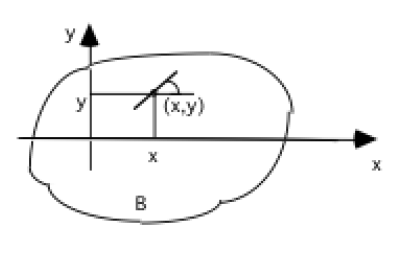
\includegraphics[width=0.8\linewidth]{Richtungsfeld.png}
    \end{center}
  \end{minipage}
  \hspace{3mm}
  \begin{minipage}{0.45\linewidth}
    \begin{center}
    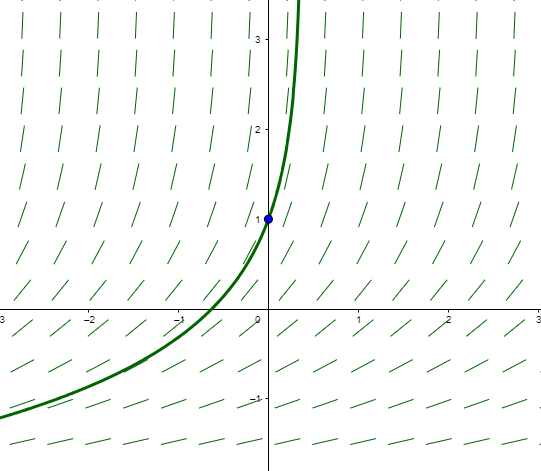
\includegraphics[width=0.8\linewidth]{RichtungsfeldKurve.png}
    \end{center}
  \end{minipage}

  \begin{minipage}{0.45\linewidth}
    \(f(x,y)\) gibt also die Steigung der Lösungskurve am Punkt \((x,y)\) an
  \end{minipage}
  \hspace{3mm}
  \begin{minipage}{0.45\linewidth}
    Jeder Punkt ist somit die Tangente einer spezifischen Lösungskurve
  \end{minipage}
\end{definition}

\begin{definition}{Richtungsfelder von Speziellen DGL}\\
  \begin{minipage}{0.58\linewidth}
    Unbestimmtes Integral: \(y'=f(x)\)\\ das Richtungsfeld ist unabhängig von \(y\) die verschiedenen Lösungen
      unterscheiden sich nur durch eine verschiebung in \(y\)-Richtung durch die Konstante \(C\).
  \end{minipage}
  \begin{minipage}{0.4\linewidth}
    \begin{center}
      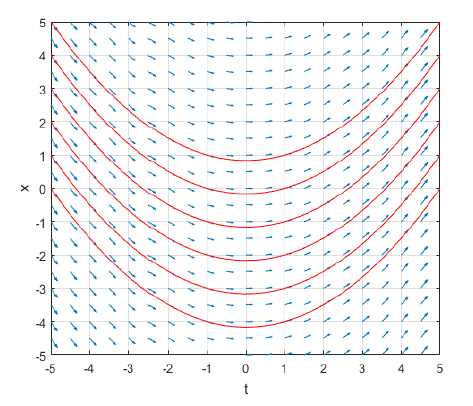
\includegraphics[width=1\linewidth]{UnbestimmtesIntegral.png}
      \end{center}
  \end{minipage}
  \begin{minipage}{0.58\linewidth}
    Autonome DGL:\(y'=f(y)\)\\ das Richtungsfeld ist unabhängig von \(x\) die Verschiedenen Lösungen gehen durch
    Verschiebung in \(x\)-Richtung in einander über.
  \end{minipage}
  \begin{minipage}{0.4\linewidth}
    \begin{center}
      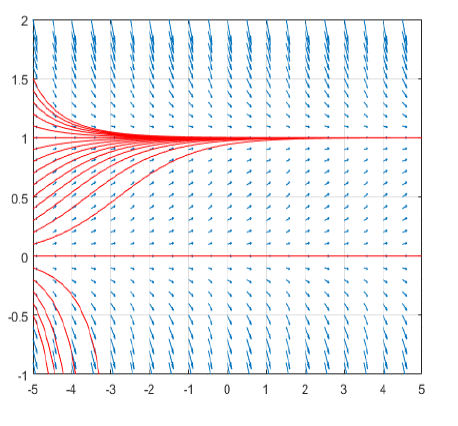
\includegraphics[width=1\linewidth]{AutonomeDGL.png}
      \end{center}
  \end{minipage}
\end{definition}






\paragraph{Numerische Verfahren}
\begin{definition}{Eulerverfahren}
  Gleichung einer beliebigen Geraden mit Steigung \(m\) am Punkt \((x_k,y_k)\):
      \[y=y_k+m\cdot(x-x_k)\]
    \begin{minipage}{0.5\linewidth}
      DGL am Punkt \((x_k,y_k)\):
      \[y=y_k+f(x_k,y_k)\cdot (x-x_k)\]
    \end{minipage}
    \begin{minipage}{0.45\linewidth}
      \begin{center}
        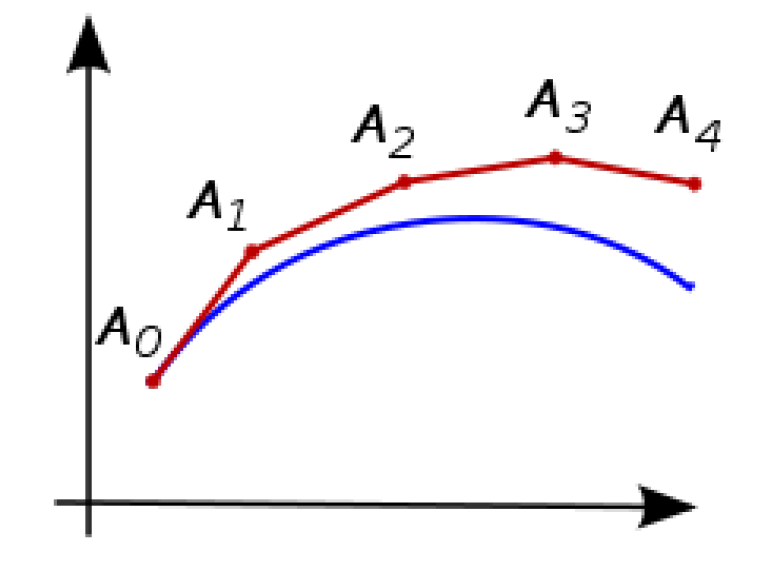
\includegraphics[width=0.7\linewidth]{Newtonverfahren.png}
        \end{center}
    \end{minipage}
  \begin{itemize}

    \item Für \(k=0 \text{ und } x=x_0\):
      \[\underbrace{y_1}_{\approx y(x_1)}=y_0+f(x_0,y_0)\cdot\underbrace{(x_1-x_0)}_{=h}\]
    \item Algorithmus für beliebige \(k\):
      \[\left\{\begin{tabular}{rcl}
	  \(x_k\)&\(=\)&\(x_0+k\cdot h\)\\
	  \(y_{k+1}\)&\(=\)&\(y_k+h\cdot f(x_k,y_k)\)
	\end{tabular}
      \right.\]
  \end{itemize}
  Problem: Die Steigung wird nur am linken Ende des Intervalls berücksichtigt!
    \\ $\Rightarrow$ Lösung: Verbesserte numerische Verfahren!
\end{definition}


\begin{definition}{Gewöhnliche Differentialgleichung n-ter Ordnung}\\
Eine Gleichung, in der Ableitungen einer unbekannten Funktion $y = y(x)$ bis zur $n$-ten Ordnung auftreten, heißt eine gewöhnliche Differentialgleichung $n$-ter Ordnung. Sie hat die explizite Form:
$$y^{(n)}(x) = f(x, y(x), y'(x), ..., y^{(n-1)}(x))$$

Gesucht sind die Lösungen $y = y(x)$ dieser Gleichung, wobei die Lösungen $y$ auf einem Intervall $[a,b]$ definiert sein sollen.

\textbf{Notationen für Ableitungen:}
$$\text{\textbf{Lagrange: }} y'(x), y''(x), y'''(x), y^{(4)}(x), ..., y^{(n)}(x)$$
$$\text{\textbf{Newton: }} \dot{y}(x), \ddot{y}(x), \dddot{y}(x), ...$$
$$\text{\textbf{Leibniz: }} \frac{dy}{dx}, \frac{d^2y}{dx^2}, \frac{d^3y}{dx^3}, ..., \frac{d^ny}{dx^n}$$
\end{definition}

\begin{definition}{Anfangswertproblem (AWP)}\\
Bei einem Anfangswertproblem für eine Differentialgleichung $n$-ter Ordnung werden der Lösungsfunktion $y = y(x)$ noch $n$ Werte vorgeschrieben:

\textbf{DGL 1. Ordnung:} \\
Gegeben ist $y'(x) = f(x, y(x))$ und der Anfangswert $y(x_0) = y_0$.
\vspace{2mm}\\
\textbf{DGL 2. Ordnung:} 
Gegeben ist $y''(x) = f(x, y(x), y'(x))$ und die Anfangswerte $y(x_0) = y_0$, $y'(x_0) = y_0'$.
\end{definition}

\begin{example2}{Beispiele aus den Naturwissenschaften}\\
\textbf{Aufgabe:} Klassifizieren Sie die folgenden DGL und geben Sie physikalische Interpretationen an.
\tcblower
\textbf{1. Radioaktiver Zerfall:}
$$\frac{dn}{dt} = -\lambda n$$
DGL 1. Ordnung, Lösung: $n(t) = n_0 e^{-\lambda t}$
\vspace{2mm}\\
\textbf{2. Freier Fall:}
$$\ddot{s}(t) = -g$$
DGL 2. Ordnung, Lösung: $s(t) = -\frac{1}{2}gt^2 + v_0 t + s_0$
\vspace{2mm}\\
\textbf{3. Harmonische Schwingung (Federpendel):}
$$m\ddot{x} = -cx \Rightarrow \ddot{x} + \frac{c}{m}x = 0$$
DGL 2. Ordnung, Lösung: $x(t) = A \sin(\omega_0 t + \varphi)$ mit $\omega_0 = \sqrt{\frac{c}{m}}$
\end{example2}

\raggedcolumns
\columnbreak

\subsection{Richtungsfelder}

\begin{concept}{Geometrische Interpretation}\\
Die DGL $y'(x) = f(x, y(x))$ gibt uns einen Zusammenhang zwischen der Steigung $y'(x)$ der gesuchten Funktion und dem Punkt $(x, y(x))$.

Im Richtungsfeld wird an jedem Punkt $(x,y)$ die Steigung $y'(x) = f(x,y)$ durch einen kleinen Pfeil dargestellt. Die Lösungskurven verlaufen stets tangential zu diesen Pfeilen.
\end{concept}

\begin{KR}{Richtungsfeld zeichnen und interpretieren}
\paragraph{Schritt 1: Steigungen berechnen}
Für eine gegebene DGL $y' = f(x,y)$ berechne für verschiedene Punkte $(x_i, y_j)$ die Steigung $f(x_i, y_j)$.

\paragraph{Schritt 2: Richtungspfeile einzeichnen}
Zeichne an jedem Punkt $(x_i, y_j)$ einen kleinen Pfeil mit der Steigung $f(x_i, y_j)$.

\paragraph{Schritt 3: Lösungskurven folgen}
Von einem Anfangspunkt $(x_0, y_0)$ ausgehend folge den Richtungspfeilen, um die Lösungskurve zu approximieren.

\paragraph{Schritt 4: Python-Implementierung}
Verwende \texttt{numpy.meshgrid()} und \texttt{pyplot.quiver()} zur automatischen Darstellung.
\end{KR}

\begin{example2}{Richtungsfeld interpretieren}\\
\textbf{Aufgabe:} Zeichnen Sie das Richtungsfeld für $\frac{dy}{dt} = -\frac{1}{2} \cdot y \cdot t^2$ und bestimmen Sie die Lösungskurve für $y(0) = 3$.
\tcblower
\textbf{Lösung:}

\textbf{Steigungen an ausgewählten Punkten:}
\begin{center}
\begin{tabular}{|c|c|c|c|c|}
\hline
$\frac{dy}{dt}$ & $t=0$ & $t=1$ & $t=2$ & $t=3$ \\
\hline
$y=0$ & 0 & 0 & 0 & 0 \\
\hline
$y=1$ & 0 & -0.5 & -2 & -4.5 \\
\hline
$y=2$ & 0 & -1 & -4 & -9 \\
\hline
$y=3$ & 0 & -1.5 & -6 & -13.5 \\
\hline
\end{tabular}
\end{center}

Die Lösungskurve für $y(0) = 3$ folgt den Richtungspfeilen und zeigt exponentiellen Abfall für $t > 0$.
\end{example2}

\raggedcolumns
\pagebreak

\subsection{Numerische Lösungsverfahren}

\subsubsection{Das Euler-Verfahren}

\begin{theorem}{Klassisches Euler-Verfahren}\\
Gegeben sei das AWP $y' = f(x,y)$ mit $y(a) = y_0$ auf dem Intervall $[a,b]$.

Das Euler-Verfahren mit Schrittweite $h = \frac{b-a}{n}$ lautet:
$$x_{i+1} = x_i + h$$
$$y_{i+1} = y_i + h \cdot f(x_i, y_i)$$

wobei $x_0 = a$, $x_i = a + ih$ für $i = 0, ..., n-1$ und $y_0$ der gegebene Anfangswert ist.
\end{theorem}

\begin{concept}{Idee des Euler-Verfahrens}\\
Das Euler-Verfahren folgt der Tangente im Punkt $(x_i, y_i)$ mit der Steigung $f(x_i, y_i)$ um die Schrittweite $h$. Es ist das einfachste Einschrittverfahren mit Konvergenzordnung $p = 1$.
\end{concept}

\begin{KR}{Euler-Verfahren anwenden}
\paragraph{Schritt 1: Parameter bestimmen}
Gegeben: AWP $y' = f(x,y)$, $y(a) = y_0$, Intervall $[a,b]$, Anzahl Schritte $n$
Berechne: $h = \frac{b-a}{n}$

\paragraph{Schritt 2: Startwerte setzen}
$x_0 = a$, $y_0 = $ gegebener Anfangswert

\paragraph{Schritt 3: Iteration}
Für $i = 0, 1, ..., n-1$:
\begin{itemize}
    \item Berechne $f(x_i, y_i)$
    \item Setze $x_{i+1} = x_i + h$
    \item Setze $y_{i+1} = y_i + h \cdot f(x_i, y_i)$
\end{itemize}

\paragraph{Schritt 4: Lösung interpretieren}
Die Punkte $(x_i, y_i)$ approximieren die Lösung $y(x)$ an den Stützstellen.
\end{KR}

\begin{example2}{Euler-Verfahren berechnen}\\
\textbf{Aufgabe:} Lösen Sie $\frac{dy}{dx} = \frac{x^2}{y}$ mit $y(0) = 2$ auf dem Intervall $[0, 1.4]$ mit $h = 0.7$ (Euler-Verfahren).
\tcblower
\textbf{Lösung:}

\textbf{Parameter:} $n = 2$, $h = 0.7$, $f(x,y) = \frac{x^2}{y}$

\textbf{Iteration:}
\begin{itemize}
    \item $i = 0$: $x_0 = 0$, $y_0 = 2$
    \item $f(0, 2) = \frac{0^2}{2} = 0$
    \item $x_1 = 0 + 0.7 = 0.7$, $y_1 = 2 + 0.7 \cdot 0 = 2$
\end{itemize}

\begin{itemize}
    \item $i = 1$: $x_1 = 0.7$, $y_1 = 2$
    \item $f(0.7, 2) = \frac{0.7^2}{2} = 0.245$
    \item $x_2 = 0.7 + 0.7 = 1.4$, $y_2 = 2 + 0.7 \cdot 0.245 = 2.1715$
\end{itemize}

\textbf{Exakte Lösung:} $y(x) = \sqrt{\frac{2x^3}{3} + 4}$
$y(1.4) = \sqrt{\frac{2 \cdot 1.4^3}{3} + 4} = 2.253$

\textbf{Absoluter Fehler:} $|2.253 - 2.1715| = 0.0815$
\end{example2}

\subsubsection{Verbesserte Euler-Verfahren}

\begin{theorem}{Mittelpunkt-Verfahren}\\
Das Mittelpunkt-Verfahren berechnet die Steigung in der Mitte des Intervalls:
$$x_{h/2} = x_i + \frac{h}{2}$$
$$y_{h/2} = y_i + \frac{h}{2} \cdot f(x_i, y_i)$$
$$x_{i+1} = x_i + h$$
$$y_{i+1} = y_i + h \cdot f(x_{h/2}, y_{h/2})$$

Konvergenzordnung: $p = 2$
\end{theorem}

\begin{corollary}{Modifiziertes Euler-Verfahren (Heun-Verfahren)}\\
Das modifizierte Euler-Verfahren verwendet den Durchschnitt zweier Steigungen:
$$k_1 = f(x_i, y_i)$$
$$k_2 = f(x_i + h, y_i + h \cdot k_1)$$
$$x_{i+1} = x_i + h$$
$$y_{i+1} = y_i + h \cdot \frac{k_1 + k_2}{2}$$

Konvergenzordnung: $p = 2$
\end{corollary}

\begin{example2}{Vergleich der Euler-Verfahren}\\
\textbf{Aufgabe:} Lösen Sie das AWP aus dem vorigen Beispiel mit Mittelpunkt- und modifiziertem Euler-Verfahren. Vergleichen Sie die Genauigkeit.
\tcblower
\textbf{Mittelpunkt-Verfahren:}
\begin{itemize}
    \item $x_{1/2} = 0.35$, $y_{1/2} = 2$, $f(0.35, 2) = 0.061$
    \item $y_1 = 2 + 0.7 \cdot 0.061 = 2.043$
    \item $x_{3/2} = 1.05$, $y_{3/2} = 2.128$, $f(1.05, 2.128) = 0.518$
    \item $y_2 = 2.043 + 0.7 \cdot 0.518 = 2.406$
\end{itemize}
\vspace{2mm}
\textbf{Modifiziertes Euler-Verfahren:}
\begin{itemize}
    \item $k_1 = 0$, $k_2 = f(0.7, 2) = 0.245$
    \item $y_1 = 2 + 0.7 \cdot \frac{0 + 0.245}{2} = 2.086$
    \item $k_1 = 0.245$, $k_2 = f(1.4, 2.257) = 0.866$
    \item $y_2 = 2.086 + 0.7 \cdot \frac{0.245 + 0.866}{2} = 2.475$
\end{itemize}
\vspace{2mm}
\textbf{Fehlervergleich bei $x = 1.4$:}
\begin{itemize}
    \item Exakt: $y(1.4) = 2.253$
    \item Euler: $|2.253 - 2.172| = 0.081$
    \item Mittelpunkt: $|2.253 - 2.406| = 0.153$
    \item Modifiziert: $|2.253 - 2.475| = 0.222$
\end{itemize}
\end{example2}

\subsubsection{Runge-Kutta Verfahren}

\begin{theorem}{Klassisches vierstufiges Runge-Kutta Verfahren}\\
Das klassische Runge-Kutta Verfahren verwendet vier Steigungen und hat Konvergenzordnung $p = 4$:
\vspace{-2mm}\\
$$k_1 = f(x_i, y_i), \quad
k_2 = f(x_i + \frac{h}{2}, y_i + \frac{h}{2} k_1)$$
$$k_3 = f(x_i + \frac{h}{2}, y_i + \frac{h}{2} k_2), \quad
k_4 = f(x_i + h, y_i + h k_3)$$
$$x_{i+1} = x_i + h, \quad
y_{i+1} = y_i + h \cdot \frac{1}{6}(k_1 + 2k_2 + 2k_3 + k_4)$$
\end{theorem}

\begin{concept}{Butcher-Schema}
    Runge-Kutta Verfahren werden durch Butcher-Schemata charakterisiert:

    \begin{minipage}{0.45\textwidth}
        \begin{center}
        \begin{tabular}{c|cccc}
        0 & & & & \\
        $\frac{1}{2}$ & $\frac{1}{2}$ & & & \\
        $\frac{1}{2}$ & 0 & $\frac{1}{2}$ & & \\
        1 & 0 & 0 & 1 & \\
        \hline
        & $\frac{1}{6}$ & $\frac{1}{3}$ & $\frac{1}{3}$ & $\frac{1}{6}$
        \end{tabular}
        \end{center}
    \end{minipage}
    \begin{minipage}{0.54\textwidth}
        \textbf{Interpretation:} Die erste Spalte gibt die Stufen $c_i$, 
        die zweite Spalte die Koeffizienten $a_{ij}$ für die Steigungen $k_j$ und die letzte Zeile die Gewichtung der Steigungen für die nächste Iteration an.
    \end{minipage}

\end{concept}

\begin{KR}{Runge-Kutta Verfahren anwenden}
\paragraph{Schritt 1: Steigungen berechnen}
\vspace{-2mm}
$$k_1 = f(x_i, y_i), \quad
k_2 = f(x_i + \frac{h}{2}, y_i + \frac{h}{2} k_1)$$
$$k_3 = f(x_i + \frac{h}{2}, y_i + \frac{h}{2} k_2), \quad
k_4 = f(x_i + h, y_i + h k_3)$$

\paragraph{Schritt 2: Gewichtetes Mittel bilden}
\vspace{-2mm}
$$\text{Steigung} = \frac{1}{6}(k_1 + 2k_2 + 2k_3 + k_4)$$

\paragraph{Schritt 3: Nächsten Punkt berechnen}
\vspace{-2mm}
$$x_{i+1} = x_i + h, \quad
y_{i+1} = y_i + h \cdot \text{Steigung}$$

\paragraph{Schritt 4: Iteration fortsetzen}
Wiederhole bis zum Ende des Intervalls.
\end{KR}

\begin{example2}{Runge-Kutta vs. andere Verfahren}\\
\textbf{Aufgabe:} Lösen Sie $y' = 1 - \frac{y}{t}$ mit $y(1) = 5$ für $t \in [1,6]$ mit $h = 0.01$ und vergleichen Sie mit der exakten Lösung $y(t) = \frac{t^2 + 9}{2t}$.

\begin{lstlisting}[language=Python, style=basesmol]
def runge_kutta_4(f, a, b, n, y0):
    h = (b - a) / n
    x = a
    y = y0
    
    for i in range(n):
        k1 = f(x, y)
        k2 = f(x + h/2, y + h/2 * k1)
        k3 = f(x + h/2, y + h/2 * k2)
        k4 = f(x + h, y + h * k3)
        
        x += h
        y += h * (k1 + 2*k2 + 2*k3 + k4) / 6
        
    return x, y
\end{lstlisting}

\textbf{Fehlervergleich bei $t = 6$:}
\begin{itemize}
    \item Exakt: $y(6) = 3.25$
    \item Euler: Fehler $\approx 0.1$
    \item Runge-Kutta: Fehler $\approx 10^{-6}$
\end{itemize}
\end{example2}

\subsection{Systeme von Differentialgleichungen}

\begin{concept}{DGL höherer Ordnung $\rightarrow$ System 1. Ordnung}\\
Jede DGL $n$-ter Ordnung kann in ein System von $n$ DGL 1. Ordnung umgewandelt werden durch Einführung von Hilfsvariablen für die Ableitungen.
\end{concept}

\begin{KR}{DGL höherer Ordnung auf System 1. Ordnung zurückführen}
\paragraph{Schritt 1: Nach höchster Ableitung auflösen}
Bringe die DGL in die Form $y^{(n)} = f(x, y, y', ..., y^{(n-1)})$.
\vspace{2mm}\\
\begin{minipage}{0.45\linewidth}
\paragraph{Schritt 2: Hilfsvariablen einführen}
\vspace{-3mm}
$$z_1(x) = y(x)$$
$$z_2(x) = y'(x)$$
$$z_3(x) = y''(x)$$
$$...$$
$$z_n(x) = y^{(n-1)}(x)$$
\end{minipage}
\hspace{2mm}
\begin{minipage}{0.5\linewidth}
\paragraph{Schritt 3: System aufstellen}
\vspace{-3mm}
$$z_1' = z_2$$
$$z_2' = z_3$$
$$...$$
$$z_{n-1}' = z_n$$
$$z_n' = f(x, z_1, z_2, ..., z_n)$$
\end{minipage}

\paragraph{Schritt 4: Vektorielle Schreibweise}
$\mathbf{z}' = \mathbf{f}(x, \mathbf{z})$ mit $\mathbf{z}(x_0) = \begin{psmallmatrix} y(x_0) \\ y'(x_0) \\ \vdots \\ y^{(n-1)}(x_0) \end{psmallmatrix}$
\end{KR}

\begin{example2}{Landende Boeing - DGL 2. Ordnung}\\
\textbf{Aufgabe:} Eine Boeing 737-200 landet mit $v_0 = 100$ m/s und erfährt die Bremskraft $F = -5\dot{x}^2 - 570000$. Die Bewegungsgleichung ist:
$$m\ddot{x} = -5\dot{x}^2 - 570000$$
mit $m = 97000$ kg. Formen Sie in ein System 1. Ordnung um.
\tcblower
\textbf{Schritt 1:} Nach $\ddot{x}$ auflösen:
$$\ddot{x} = \frac{-5\dot{x}^2 - 570000}{97000}$$

\textbf{Schritt 2:} Hilfsvariablen:
$$z_1(t) = x(t) \quad \text{(Position)}$$
$$z_2(t) = \dot{x}(t) = v(t) \quad \text{(Geschwindigkeit)}$$

\textbf{Schritt 3:} System 1. Ordnung:
$$z_1' = z_2$$
$$z_2' = \frac{-5z_2^2 - 570000}{97000}$$

\textbf{Schritt 4:} Anfangsbedingungen:
$$\mathbf{z}(0) = \begin{psmallmatrix} 0 \\ 100 \end{psmallmatrix}$$

Das System kann nun mit Runge-Kutta gelöst werden.
\end{example2}

\begin{example2}{Raketenbewegung}\\
\textbf{Aufgabe:} Die Bewegungsgleichung einer Rakete lautet:
$$a(t) = \ddot{h}(t) = v_{rel} \cdot \frac{\mu}{m_A - \mu \cdot t} - g$$

mit $v_{rel} = 2600$ m/s, $m_A = 300000$ kg, $m_E = 80000$ kg, $t_E = 190$ s.

Berechnen Sie Geschwindigkeit und Höhe als Funktion der Zeit.
\tcblower
\textbf{Parameter:} $\mu = \frac{m_A - m_E}{t_E} = \frac{220000}{190} = 1158$ kg/s

\textbf{System 1. Ordnung:}
$$z_1' = z_2 \quad \text{(Höhe)}$$
$$z_2' = 2600 \cdot \frac{1158}{300000 - 1158t} - 9.81 \quad \text{(Geschwindigkeit)}$$

\textbf{Anfangsbedingungen:} $z_1(0) = 0$, $z_2(0) = 0$

\textbf{Numerische Lösung mit Trapezregel:}
$$v(t) = \int_0^t a(\tau) d\tau$$
$$h(t) = \int_0^t v(\tau) d\tau$$

\textbf{Analytische Vergleichslösung:}
$$v(t) = v_{rel} \ln(\frac{m_A}{m_A - \mu t}) - gt$$
$$h(t) = -\frac{v_{rel}(m_A - \mu t)}{\mu} \ln(\frac{m_A}{m_A - \mu t}) + v_{rel} t - \frac{1}{2}gt^2$$

\textbf{Ergebnisse nach 190s:}
\begin{itemize}
    \item Geschwindigkeit: $\approx 2500$ m/s
    \item Höhe: $\approx 180$ km
    \item Beschleunigung: $\approx 2.5g$
\end{itemize}
\end{example2}

\raggedcolumns
\columnbreak

\subsection{Stabilität}

\begin{concept}{Stabilitätsproblem}\\
Bei der numerischen Lösung von DGL kann es vorkommen, dass der numerische Fehler unbeschränkt wächst, unabhängig von der Schrittweite $h$. Dies führt zu \textbf{instabilen} Lösungen.

Die Stabilität hängt ab von:
\begin{itemize}
    \item Dem verwendeten Verfahren
    \item Der Schrittweite $h$
    \item Dem spezifischen Anfangswertproblem
\end{itemize}
\end{concept}

\begin{definition}{Stabilitätsfunktion}\\
Für die DGL $y' = -\alpha y$ (mit $\alpha > 0$) kann die numerische Lösung in der Form
$$y_{i+1} = g(h\alpha) \cdot y_i$$
geschrieben werden. Die Funktion $g(z)$ heißt \textbf{Stabilitätsfunktion} des Verfahrens.

Das offene Intervall $z \in (0, \alpha)$, in dem $|g(z)| < 1$ gilt, bezeichnet man als \textbf{Stabilitätsintervall}.
\end{definition}

\begin{example2}{Stabilität des Euler-Verfahrens}\\
\textbf{Aufgabe:} Untersuchen Sie die Stabilität des Euler-Verfahrens für $y' = -2.5y$ mit $y(0) = 1$.
\tcblower
\textbf{Euler-Verfahren:} $y_{i+1} = y_i - h \cdot 2.5 y_i = y_i(1 - 2.5h)$

\textbf{Stabilitätsfunktion:} $g(z) = 1 - z$ mit $z = 2.5h$

\textbf{Stabilitätsbedingung:} $|1 - 2.5h| < 1$
$\Rightarrow 0 < 2.5h < 2 \Rightarrow 0 < h < 0.8$

\textbf{Verhalten:}
\begin{itemize}
    \item $h = 0.2$: Stabile Lösung (exponentieller Abfall)
    \item $h = 0.85$: Instabile Lösung (Oszillation mit wachsender Amplitude)
\end{itemize}

\textbf{Exakte Lösung:} $y(x) = e^{-2.5x}$ (streng monoton fallend)
\end{example2}

\begin{theorem}{Praktische Hinweise zur Stabilität:}
\begin{itemize}
    \item \textbf{Schrittweiten-Kontrolle:} Beginne mit kleiner Schrittweite und prüfe Konvergenz
    \item \textbf{Verfahrensvergleich:} Teste verschiedene Verfahren und vergleiche Ergebnisse
    \item \textbf{Analytische Kontrolle:} Vergleiche mit bekannten analytischen Lösungen
    \item \textbf{Steife DGL:} Verwende implizite Verfahren für steife Probleme
    \item \textbf{Python-Tools:} Nutze \texttt{scipy.integrate.solve\_ivp()} für robuste Implementierungen
\end{itemize}
\end{theorem}

\subsection{Python-Implementierung}

\begin{code}{DGL-Löser in Python}
Standard-Bibliothek für DGL-Probleme:
\begin{lstlisting}[language=Python, style=basesmol]
from scipy.integrate import solve_ivp
import numpy as np
import matplotlib.pyplot as plt

def f(t, y): # DGL: y' = -2*y + sin(t)
    return -2*y + np.sin(t)

# Anfangswertproblem loesen
sol = solve_ivp(f, [0, 5], [1], dense_output=True)
# Losung plotten
t = np.linspace(0, 5, 100)
y = sol.sol(t)
plt.plot(t, y[0])
plt.xlabel('t')
plt.ylabel('y(t)')
plt.title('Numerische Loesung der DGL')
plt.show()
\end{lstlisting}

\textbf{Verfügbare Methoden:}
\begin{itemize}
    \item \texttt{'RK45'}: Runge-Kutta 5(4) (Standard)
    \item \texttt{'RK23'}: Runge-Kutta 3(2)
    \item \texttt{'DOP853'}: Runge-Kutta 8. Ordnung
    \item \texttt{'Radau'}: Implizites Runge-Kutta
    \item \texttt{'BDF'}: Backward Differentiation (für steife DGL)
    \item \texttt{'LSODA'}: Automatische Steifigkeits-Erkennung
\end{itemize}
\end{code}

\begin{KR}{Eigene DGL-Löser implementieren}
\paragraph{Schritt 1: Grundstruktur}
\begin{lstlisting}[language=Python, style=basesmol]
def runge_kutta_4(f, a, b, n, y0):
    h = (b - a) / n
    x = np.linspace(a, b, n+1)
    y = np.zeros(n+1) 
# erweitert fuer Systeme: y = np.zeros((n+1, len(y0)))
    y[0] = y0
    
    for i in range(n):
        k1 = f(x[i], y[i])
        k2 = f(x[i] + h/2, y[i] + h/2 * k1)
        k3 = f(x[i] + h/2, y[i] + h/2 * k2)
        k4 = f(x[i] + h, y[i] + h * k3)
        
        y[i+1] = y[i] + h/6 * (k1 + 2*k2 + 2*k3 + k4)
    
    return x, y
\end{lstlisting}

\paragraph{Schritt 2: Richtungsfeld visualisieren}
\begin{lstlisting}[language=Python, style=basesmol]
def plot_direction_field(f, xmin, xmax, ymin, ymax, hx, hy):
    x = np.arange(xmin, xmax, hx)
    y = np.arange(ymin, ymax, hy)
    X, Y = np.meshgrid(x, y)
    
    DX = np.ones_like(X)
    DY = f(X, Y)
    
    plt.quiver(X, Y, DX, DY, alpha=0.6)
    plt.xlabel('x')
    plt.ylabel('y')
    plt.title('Richtungsfeld')
\end{lstlisting}
\end{KR}

\subsection{Fehlerordnung und Konvergenz}

\begin{definition}{Lokaler und globaler Fehler}\\
\textbf{Lokaler Fehler:} Der Fehler nach einer Iteration\\
$\varphi(x_i, h) := y(x_{i+1}) - y_{i+1}$

\textbf{Globaler Fehler:} Der Fehler nach $n$ Iterationen
$y(x_n) - y_n$

\textbf{Konsistenzordnung $p$:} \\ Ein Verfahren hat Konsistenzordnung $p$, falls
$|\varphi(x_i, h)| \leq C \cdot h^{p+1}$

\textbf{Konvergenzordnung $p$:} \\ Ein Verfahren hat Konvergenzordnung $p$, falls
$|y(x_n) - y_n| \leq C \cdot h^p$
\end{definition}

\begin{concept}{Konvergenzordnungen der Verfahren}
\begin{itemize}
    \item \textbf{Euler-Verfahren:} Konvergenzordnung $p = 1$
    \item \textbf{Mittelpunkt-Verfahren:} Konvergenzordnung $p = 2$
    \item \textbf{Modifiziertes Euler-Verfahren:} Konvergenzordnung $p = 2$
    \item \textbf{Klassisches Runge-Kutta:} Konvergenzordnung $p = 4$
\end{itemize}

\textbf{Praktische Bedeutung:} Bei Halbierung der Schrittweite $h$ reduziert sich der Fehler um den Faktor $2^p$.
\end{concept}

\begin{example2}{Konvergenzverhalten untersuchen}\\
\textbf{Aufgabe:} Untersuchen Sie das Konvergenzverhalten verschiedener Verfahren für $\frac{dy}{dx} = \frac{x^2}{y}$ mit $y(0) = 2$ auf $[0, 10]$.
\tcblower
\textbf{Exakte Lösung:} $y(x) = \sqrt{\frac{2x^3}{3} + 4}$

\textbf{Fehler bei $x = 10$ für verschiedene $h$:}

\begin{center}
\begin{tabular}{|c|c|c|c|c|}
\hline
$h$ & Euler & Mittelpunkt & Mod. Euler & Runge-Kutta \\
\hline
0.1 & $10^{-1}$ & $10^{-2}$ & $10^{-2}$ & $10^{-5}$ \\
\hline
0.05 & $5 \times 10^{-2}$ & $2.5 \times 10^{-3}$ & $2.5 \times 10^{-3}$ & $6 \times 10^{-7}$ \\
\hline
0.025 & $2.5 \times 10^{-2}$ & $6 \times 10^{-4}$ & $6 \times 10^{-4}$ & $4 \times 10^{-8}$ \\
\hline
\end{tabular}
\end{center}

\textbf{Beobachtung:} Bei Halbierung von $h$:
\begin{itemize}
    \item Euler: Fehler halbiert sich (Ordnung 1)
    \item Mittelpunkt/Mod. Euler: Fehler viertelt sich (Ordnung 2)
    \item Runge-Kutta: Fehler wird um Faktor 16 kleiner (Ordnung 4)
\end{itemize}
\end{example2}

\subsection{Spezielle Anwendungen}

\begin{example2}{Schwingungsgleichung - Gekoppeltes System}\\
\textbf{Aufgabe:} Lösen Sie die Schwingungsgleichung $\ddot{x} + \omega^2 x = 0$ mit $x(0) = 1$, $\dot{x}(0) = 0$ und $\omega = 2$.
\tcblower
\textbf{System 1. Ordnung:}
$z_1' = z_2$
$z_2' = -\omega^2 z_1 = -4z_1$

\textbf{Anfangsbedingungen:} $z_1(0) = 1$, $z_2(0) = 0$

\textbf{Analytische Lösung:} $x(t) = \cos(2t)$

\textbf{Numerische Implementierung:}
\begin{lstlisting}[language=Python, style=basesmol]
def harmonic_oscillator(t, z): # z[0] = x, z[1] = dx/dt
    return [z[1], -4*z[0]]

# Losung mit scipy
sol = solve_ivp(harmonic_oscillator, [0, 10], [1, 0], 
                method='RK45', dense_output=True)

t = np.linspace(0, 10, 1000)
z = sol.sol(t)
x_num = z[0]
x_exact = np.cos(2*t)
plt.plot(t, x_num, 'b-', label='Numerisch')
plt.plot(t, x_exact, 'r--', label='Exakt')
plt.legend()
\end{lstlisting}

\textbf{Energieerhaltung prüfen:} 
$E = \frac{1}{2}\dot{x}^2 + \frac{1}{2}\omega^2 x^2 = \text{const}$
\end{example2}

\begin{example2}{Populationsdynamik - Logistisches Wachstum}\\
\textbf{Aufgabe:} Das logistische Wachstumsmodell lautet:
$\frac{dP}{dt} = rP(1 - \frac{P}{K})$
mit Wachstumsrate $r = 0.1$ und Kapazität $K = 1000$. Anfangspopulation: $P(0) = 50$.
\tcblower
\textbf{Analytische Lösung:}
$P(t) = \frac{K}{1 + (\frac{K}{P_0} - 1)e^{-rt}}$

\textbf{Numerische Lösung:}
\begin{lstlisting}[language=Python, style=basesmol]
def logistic_growth(t, P, r=0.1, K=1000):
    return r * P * (1 - P/K)
# Parameter
r, K, P0 = 0.1, 1000, 50
# Numerische Loesung
sol = solve_ivp(lambda t, P: logistic_growth(t, P, r, K), 
                [0, 100], [P0], dense_output=True)
# Analytische Loesung
def P_exact(t):
    return K / (1 + (K/P0 - 1) * np.exp(-r*t))

t = np.linspace(0, 100, 1000)
P_num = sol.sol(t)[0]
P_ana = P_exact(t)

plt.plot(t, P_num, 'b-', label='Numerisch')
plt.plot(t, P_ana, 'r--', label='Analytisch')
plt.axhline(y=K, color='k', linestyle=':', label='Kapazitaet K')
plt.xlabel('Zeit t')
plt.ylabel('Population P(t)')
plt.legend()
\end{lstlisting}

\textbf{Charakteristisches Verhalten:} Exponentielles Wachstum für kleine $P$, Sättigung bei $K$.
\end{example2}

\begin{example2}{Prüfungsaufgabe 8.1 - Vergleich numerischer Verfahren}\\
\textbf{Aufgabe:} Lösen Sie das Anfangswertproblem:
$\frac{dy}{dx} = x + y^2, \quad y(0) = 0$

auf dem Intervall $[0, 1]$ mit Schrittweite $h = 0.2$.

a) Verwenden Sie das Euler-Verfahren
b) Verwenden Sie das klassische Runge-Kutta Verfahren  
c) Vergleichen Sie die Genauigkeit bei $x = 1$
d) Welche Konvergenzordnung erwarten Sie?
\tcblower
\textbf{a) Euler-Verfahren:}
$f(x,y) = x + y^2$, $h = 0.2$, $n = 5$

\textbf{Iteration 0 $\rightarrow$ 1:}
$x_0 = 0, y_0 = 0$
$f(0, 0) = 0 + 0^2 = 0$
$x_1 = 0.2, y_1 = 0 + 0.2 \cdot 0 = 0$

\textbf{Iteration 1 $\rightarrow$ 2:}
$x_1 = 0.2, y_1 = 0$
$f(0.2, 0) = 0.2 + 0^2 = 0.2$
$x_2 = 0.4, y_2 = 0 + 0.2 \cdot 0.2 = 0.04$

\textbf{Iteration 2 $\rightarrow$ 3:}
$x_2 = 0.4, y_2 = 0.04$
$f(0.4, 0.04) = 0.4 + 0.04^2 = 0.4016$
$x_3 = 0.6, y_3 = 0.04 + 0.2 \cdot 0.4016 = 0.1203$

\textbf{Iteration 3 $\rightarrow$ 4:}
$x_3 = 0.6, y_3 = 0.1203$
$f(0.6, 0.1203) = 0.6 + 0.1203^2 = 0.6145$
$x_4 = 0.8, y_4 = 0.1203 + 0.2 \cdot 0.6145 = 0.2432$

\textbf{Iteration 4 $\rightarrow$ 5:}
$x_4 = 0.8, y_4 = 0.2432$
$f(0.8, 0.2432) = 0.8 + 0.2432^2 = 0.8591$
$x_5 = 1.0, y_5 = 0.2432 + 0.2 \cdot 0.8591 = 0.4150$

\textbf{Euler-Ergebnis:} $y(1) \approx 0.4150$

\textbf{b) Runge-Kutta Verfahren:}

\textbf{Schritt 0 $\rightarrow$ 1:} $x_0 = 0, y_0 = 0$
$k_1 = f(0, 0) = 0$
$k_2 = f(0.1, 0) = 0.1$
$k_3 = f(0.1, 0.01) = 0.1 + 0.01^2 = 0.1001$
$k_4 = f(0.2, 0.02002) = 0.2 + 0.02002^2 = 0.2004$
$y_1 = 0 + \frac{0.2}{6}(0 + 2 \cdot 0.1 + 2 \cdot 0.1001 + 0.2004) = 0.0200$

\textbf{Schritt 1 $\rightarrow$ 2:} $x_1 = 0.2, y_1 = 0.0200$
$k_1 = f(0.2, 0.0200) = 0.2 + 0.0004 = 0.2004$
$k_2 = f(0.3, 0.0400) = 0.3 + 0.0016 = 0.3016$
$k_3 = f(0.3, 0.0502) = 0.3 + 0.0025 = 0.3025$
$k_4 = f(0.4, 0.0805) = 0.4 + 0.0065 = 0.4065$
$y_2 = 0.0200 + \frac{0.2}{6}(0.2004 + 2 \cdot 0.3016 + 2 \cdot 0.3025 + 0.4065) = 0.0801$

Fortführung analog...

\textbf{Runge-Kutta Ergebnisse:}
$y_1 = 0.0200, y_2 = 0.0801, y_3 = 0.1806, y_4 = 0.3214, y_5 = 0.5027$

\textbf{Runge-Kutta-Ergebnis:} $y(1) \approx 0.5027$

\textbf{c) Genauigkeitsvergleich:}
Für diese DGL gibt es keine einfache analytische Lösung, aber numerische Referenzlösungen mit sehr kleiner Schrittweite ergeben: $y(1) \approx 0.5463$

Fehler:
\begin{itemize}
    \item Euler: $|0.5463 - 0.4150| = 0.1313$
    \item Runge-Kutta: $|0.5463 - 0.5027| = 0.0436$
\end{itemize}

Das Runge-Kutta Verfahren ist etwa 3-mal genauer.

\textbf{d) Konvergenzordnung:}
\begin{itemize}
    \item Euler-Verfahren: Konvergenzordnung $p = 1$
    \item Runge-Kutta 4: Konvergenzordnung $p = 4$
\end{itemize}

Bei Halbierung der Schrittweite erwarten wir:
\begin{itemize}
    \item Euler: Fehler halbiert sich
    \item RK4: Fehler wird um Faktor 16 kleiner
\end{itemize}
\end{example2}

\begin{example2}{Prüfungsaufgabe 8.2 - System von DGL}\\
\textbf{Aufgabe:} Ein Satellit kreist um die Erde. Seine Bewegung wird beschrieben durch:
$\ddot{x} = -\frac{GM x}{(x^2 + y^2)^{3/2}}, \quad \ddot{y} = -\frac{GM y}{(x^2 + y^2)^{3/2}}$

mit $GM = 3.986 \times 10^{14}$ m³/s².

Anfangsbedingungen: $x(0) = 7000$ km, $y(0) = 0$, $\dot{x}(0) = 0$, $\dot{y}(0) = 7500$ m/s

a) Formen Sie in ein System 1. Ordnung um
b) Implementieren Sie einen Schritt des Mittelpunkt-Verfahrens mit $h = 10$ s
c) Interpretieren Sie die Bewegung physikalisch
\tcblower
\textbf{a) System 1. Ordnung:}
Einführung der Hilfsvariablen:
$z_1 = x$ (Position x)
$z_2 = \dot{x}$ (Geschwindigkeit x)  
$z_3 = y$ (Position y)
$z_4 = \dot{y}$ (Geschwindigkeit y)

System:
$z_1' = z_2$
$z_2' = -\frac{GM z_1}{(z_1^2 + z_3^2)^{3/2}}$
$z_3' = z_4$  
$z_4' = -\frac{GM z_3}{(z_1^2 + z_3^2)^{3/2}}$

Vektorschreibweise:
$\mathbf{z}' = \mathbf{f}(t, \mathbf{z}) = \begin{psmallmatrix}
z_2 \\
-\frac{GM z_1}{(z_1^2 + z_3^2)^{3/2}} \\
z_4 \\
-\frac{GM z_3}{(z_1^2 + z_3^2)^{3/2}}
\end{psmallmatrix}$

\textbf{b) Mittelpunkt-Verfahren:}

\textbf{Anfangswerte:} $\mathbf{z}(0) = \begin{psmallmatrix} 7 \times 10^6 \\ 0 \\ 0 \\ 7500 \end{psmallmatrix}$ (in SI-Einheiten)

\textbf{Schritt 1:} Berechne $\mathbf{f}(0, \mathbf{z}_0)$
$r_0 = \sqrt{(7 \times 10^6)^2 + 0^2} = 7 \times 10^6$ m

$a_0 = \frac{GM}{r_0^2} = \frac{3.986 \times 10^{14}}{(7 \times 10^6)^2} = 8.13$ m/s²
$\mathbf{f}(0, \mathbf{z}_0) = \begin{psmallmatrix} 0 \\ -8.13 \\ 7500 \\ 0 \end{psmallmatrix}$

\textbf{Schritt 2:} Mittelpunkt berechnen

$\mathbf{z}_{1/2} = \mathbf{z}_0 + \frac{h}{2} \mathbf{f}(0, \mathbf{z}_0) = \begin{psmallmatrix} 7 \times 10^6 \\ 0 \\ 0 \\ 7500 \end{psmallmatrix} + 5 \begin{psmallmatrix} 0 \\ -8.13 \\ 7500 \\ 0 \end{psmallmatrix}$
$= \begin{psmallmatrix} 7 \times 10^6 \\ -40.65 \\ 37500 \\ 7500 \end{psmallmatrix}$

\textbf{Schritt 3:} $\mathbf{f}$ am Mittelpunkt berechnen

$r_{1/2} = \sqrt{(7 \times 10^6)^2 + (37500)^2} = 7.0001 \times 10^6$ m
$\mathbf{f}(5, \mathbf{z}_{1/2}) = \begin{psmallmatrix} -40.65 \\ -8.128 \\ 7500 \\ -0.043 \end{psmallmatrix}$

\textbf{Schritt 4:} Neuen Punkt berechnen

$\mathbf{z}_1 = \mathbf{z}_0 + h \cdot \mathbf{f}(5, \mathbf{z}_{1/2}) = \begin{psmallmatrix} 7 \times 10^6 - 406.5 \\ -81.28 \\ 75000 \\ 7499.57 \end{psmallmatrix}$
$= \begin{psmallmatrix} 6.9996 \times 10^6 \\ -81.28 \\ 75000 \\ 7499.57 \end{psmallmatrix}$

\textbf{c) Physikalische Interpretation:}
\begin{itemize}
    \item Der Satellit startet in 7000 km Höhe ($\approx$ 400 km über Erdoberfläche)
    \item Anfangsgeschwindigkeit 7500 m/s ist nahe der Kreisbahngeschwindigkeit 
    \item Die Gravitationskraft sorgt für die zentripetale Beschleunigung
    \item Nach 10 s hat sich der Satellit bereits deutlich bewegt: $\Delta x = -406.5$ m, $\Delta y = 75000$ m
    \item Die Bahn ist eine Ellipse (oder bei passender Geschwindigkeit ein Kreis)
    \item Erhaltungsgrößen: Energie und Drehimpuls (sollten bei genauer numerischer Lösung konstant bleiben)
\end{itemize}
\end{example2}

\begin{example2}{Prüfungsaufgabe 8.3 - Stabilität und Fehleranalyse}\\
\textbf{Aufgabe:} Betrachten Sie die DGL:
$y' = -5y + \cos(x), \quad y(0) = 1$

a) Bestimmen Sie die analytische Lösung
b) Untersuchen Sie die Stabilität des Euler-Verfahrens  
c) Für welche Schrittweiten ist das Verfahren stabil?
d) Vergleichen Sie numerische und analytische Lösung für $h = 0.3$ und $h = 0.5$
\tcblower
\textbf{a) Analytische Lösung:}
Die DGL $y' + 5y = \cos(x)$ ist eine lineare DGL 1. Ordnung.

Homogene Lösung: $y_h = Ce^{-5x}$

Partikuläre Lösung durch Ansatz $y_p = A\cos(x) + B\sin(x)$:
$y_p' = -A\sin(x) + B\cos(x)$

Einsetzen: $-A\sin(x) + B\cos(x) + 5(A\cos(x) + B\sin(x)) = \cos(x)$
$(-A + 5B)\sin(x) + (B + 5A)\cos(x) = \cos(x)$

Koeffizientenvergleich:
$-A + 5B = 0 \Rightarrow A = 5B$
$B + 5A = 1 \Rightarrow B + 25B = 1 \Rightarrow B = \frac{1}{26}, A = \frac{5}{26}$

$y_p = \frac{5}{26}\cos(x) + \frac{1}{26}\sin(x)$

Allgemeine Lösung: $y = Ce^{-5x} + \frac{5}{26}\cos(x) + \frac{1}{26}\sin(x)$

Anfangsbedingung: $y(0) = C + \frac{5}{26} = 1 \Rightarrow C = \frac{21}{26}$

$y(x) = \frac{21}{26}e^{-5x} + \frac{5}{26}\cos(x) + \frac{1}{26}\sin(x)$

\textbf{b) Stabilität des Euler-Verfahrens:}
Für die Testgleichung $y' = -\alpha y$ (hier $\alpha = 5$) lautet die Stabilitätsfunktion:
$g(z) = 1 - z \quad \text{mit } z = h\alpha = 5h$

Stabilitätsbedingung: $|1 - 5h| < 1$
$-1 < 1 - 5h < 1$
$-2 < -5h < 0$
$0 < h < \frac{2}{5} = 0.4$

\textbf{c) Stabilitätsbereich:}
Das Euler-Verfahren ist stabil für $0 < h < 0.4$.

\textbf{d) Numerischer Vergleich:}

\textbf{Für $h = 0.3$ (stabil):}
Euler-Iteration mit $f(x,y) = -5y + \cos(x)$:

$x_0 = 0, y_0 = 1$
$y_1 = 1 + 0.3(-5 \cdot 1 + \cos(0)) = 1 + 0.3(-4) = -0.2$
$y_2 = -0.2 + 0.3(-5 \cdot (-0.2) + \cos(0.3)) = -0.2 + 0.3(1 + 0.955) = 0.387$
$y_3 = 0.387 + 0.3(-5 \cdot 0.387 + \cos(0.6)) = 0.387 + 0.3(-1.935 + 0.825) = 0.054$

Bei $x = 0.9$: $y_{\text{Euler}} \approx 0.054$
Analytisch: $y(0.9) = \frac{21}{26}e^{-4.5} + \frac{5}{26}\cos(0.9) + \frac{1}{26}\sin(0.9) = 0.197$

\textbf{Für $h = 0.5$ (instabil):}
$x_0 = 0, y_0 = 1$
$y_1 = 1 + 0.5(-5 \cdot 1 + 1) = 1 + 0.5(-4) = -1$
$y_2 = -1 + 0.5(-5 \cdot (-1) + \cos(0.5)) = -1 + 0.5(5 + 0.878) = 1.939$
$y_3 = 1.939 + 0.5(-5 \cdot 1.939 + \cos(1)) = 1.939 + 0.5(-9.695 + 0.540) = -2.639$

Die Lösung oszilliert mit wachsender Amplitude $\rightarrow$ instabil!

\textbf{Interpretation:}
\begin{itemize}
    \item Für $h = 0.3$: Das Verfahren ist stabil, aber nicht sehr genau
    \item Für $h = 0.5$: Das Verfahren wird instabil und divergiert
    \item Die Stabilitätsgrenze $h < 0.4$ muss eingehalten werden
    \item Der schnell abfallende Term $e^{-5x}$ macht die DGL steif
\end{itemize}
\end{example2}

\begin{example2}{Prüfungsaufgabe 8.4 - Anwendung: Populationsdynamik}\\
\textbf{Aufgabe:} Das Räuber-Beute-System wird beschrieben durch:
$\frac{dx}{dt} = ax - bxy$
$\frac{dy}{dt} = -cy + dxy$

wobei $x(t)$ die Beutepopulation und $y(t)$ die Räuberpopulation darstellt.

Parameter: $a = 1.0$, $b = 0.5$, $c = 0.75$, $d = 0.25$
Anfangsbedingungen: $x(0) = 4$, $y(0) = 4$

a) Interpretieren Sie die Gleichungen biologisch
b) Lösen Sie das System numerisch mit Runge-Kutta für $t \in [0, 15]$ mit $h = 0.1$
c) Analysieren Sie das Langzeitverhalten
d) Was passiert mit der Gesamtenergie des Systems?
\tcblower

\textbf{a) Biologische Interpretation:}
\textbf{Beutegleichung:} $\frac{dx}{dt} = ax - bxy$
\begin{itemize}
    \item $ax$: Exponentielles Wachstum der Beute bei Abwesenheit von Räubern
    \item $-bxy$: Verluste durch Räuber (proportional zu beiden Populationen)
    \item $a = 1.0$: Wachstumsrate der Beute
    \item $b = 0.5$: Effizienz der Räuber beim Beutefang
\end{itemize}

\textbf{Räubergleichung:} $\frac{dy}{dt} = -cy + dxy$
\begin{itemize}
    \item $-cy$: Exponentieller Rückgang bei Abwesenheit von Beute
    \item $dxy$: Wachstum durch erfolgreiche Jagd
    \item $c = 0.75$: Sterberate der Räuber
    \item $d = 0.25$: Effizienz der Nahrungsumwandlung
\end{itemize}

\textbf{b) Numerische Lösung:}

System in Vektorform:

$\mathbf{z}' = \mathbf{f}(t, \mathbf{z}) = \begin{psmallmatrix}
1.0 z_1 - 0.5 z_1 z_2 \\
-0.75 z_2 + 0.25 z_1 z_2
\end{psmallmatrix}$
mit $\mathbf{z}(0) = \begin{psmallmatrix} 4 \\ 4 \end{psmallmatrix}$

\textbf{Runge-Kutta Implementation (Auszug):}

\textbf{Schritt 0 $\rightarrow$ 1:} $t_0 = 0$, $\mathbf{z}_0 = \begin{psmallmatrix} 4 \\ 4 \end{psmallmatrix}$

$\mathbf{k}_1 = \mathbf{f}(0, \begin{psmallmatrix} 4 \\ 4 \end{psmallmatrix}) = \begin{psmallmatrix} 4 - 8 \\ -3 + 4 \end{psmallmatrix} = \begin{psmallmatrix} -4 \\ 1 \end{psmallmatrix}$

$\mathbf{k}_2 = \mathbf{f}(0.05, \begin{psmallmatrix} 4 - 0.2 \\ 4 + 0.05 \end{psmallmatrix}) = \mathbf{f}(0.05, \begin{psmallmatrix} 3.8 \\ 4.05 \end{psmallmatrix})$


$= \begin{psmallmatrix} 3.8 - 3.8 \cdot 4.05 \\ -3.0375 + 0.25 \cdot 3.8 \cdot 4.05 \end{psmallmatrix} = \begin{psmallmatrix} -11.59 \\ 0.81 \end{psmallmatrix}$

$\mathbf{k}_3 = \mathbf{f}(0.05, \begin{psmallmatrix} 4 - 0.58 \\ 4 + 0.041 \end{psmallmatrix}) = \begin{psmallmatrix} -11.73 \\ 0.69 \end{psmallmatrix}$

$\mathbf{k}_4 = \mathbf{f}(0.1, \begin{psmallmatrix} 4 - 1.17 \\ 4 + 0.069 \end{psmallmatrix}) = \begin{psmallmatrix} -15.77 \\ -0.23 \end{psmallmatrix}$

$\mathbf{z}_1 = \begin{psmallmatrix} 4 \\ 4 \end{psmallmatrix} + \frac{0.1}{6}\begin{psmallmatrix} -4 - 23.18 - 23.46 - 15.77 \\ 1 + 1.62 + 1.38 - 0.23 \end{psmallmatrix}$
$= \begin{psmallmatrix} 4 \\ 4 \end{psmallmatrix} + \begin{psmallmatrix} -1.11 \\ 0.063 \end{psmallmatrix} = \begin{psmallmatrix} 2.89 \\ 4.063 \end{psmallmatrix}$

\textbf{Typische Ergebnisse nach vollständiger Integration:}
\begin{center}
\begin{tabular}{|c|c|c|}
\hline
$t$ & $x(t)$ & $y(t)$ \\
\hline
0 & 4.00 & 4.00 \\
3 & 1.32 & 2.85 \\
6 & 2.67 & 1.13 \\
9 & 6.21 & 2.34 \\
12 & 3.89 & 5.67 \\
15 & 1.45 & 3.12 \\
\hline
\end{tabular}
\end{center}

\textbf{c) Langzeitverhalten:}
\begin{itemize}
    \item Das System zeigt periodische Oszillationen (Grenzzyklus)
    \item Periode: $T \approx 6.3$ Zeiteinheiten
    \item Phasenverschiebung: Räuberpopulation folgt der Beutepopulation mit Verzögerung
    \item Typischer Zyklus:
    \begin{enumerate}
        \item Viel Beute $\rightarrow$ Räuber vermehren sich
        \item Viele Räuber $\rightarrow$ Beute wird dezimiert  
        \item Wenig Beute $\rightarrow$ Räuber sterben aus
        \item Wenige Räuber $\rightarrow$ Beute erholt sich
    \end{enumerate}
\end{itemize}

\textbf{d) Erhaltungsgrößen:}
Das Lotka-Volterra System hat eine Erhaltungsgröße (Hamiltonfunktion):
$H(x,y) = d \cdot x + b \cdot y - c \cdot \ln(x) - a \cdot \ln(y)$
$= 0.25x + 0.5y - 0.75\ln(x) - \ln(y)$
\end{example2}

\begin{example2}{Prüfungsaufgabe 8.4- continued}\\
\textbf{Numerische Verifikation:}
\begin{itemize}
    \item $H(4,4) = 1 + 2 - 0.75 \cdot 1.386 - 1.386 = 0.575$
    \item Nach einer Periode sollte $H \approx 0.575$ sein
    \item Abweichungen zeigen numerische Fehler an
    \item Das System ist konservativ (keine Dämpfung)
\end{itemize}

\textbf{Praktische Bedeutung:}
Diese Gleichungen beschreiben reale Ökosysteme nur näherungsweise, da sie:
\begin{itemize}
    \item Kapazitätsgrenzen ignorieren
    \item Andere Nahrungsquellen vernachlässigen
    \item Umwelteinflüsse nicht berücksichtigen
    \item Trotzdem wichtig für das Verständnis von Populationsdynamik
\end{itemize}
\end{example2}

\subsection{Zusätzliche Musteraufgaben}

\begin{example2}{Musteraufgabe: Kombinierte Anwendung}\\
\textbf{Aufgabe:} Ein Unternehmen modelliert seine Umsatzentwicklung durch die DGL:
$\frac{dU}{dt} = 0.1U(100 - U) - S(t)$

wobei $U(t)$ der Umsatz in Millionen € und $S(t) = 20\sin(2\pi t)$ saisonale Schwankungen sind.

a) Klassifizieren Sie die DGL
b) Für konstante Terme ($S = 0$): Bestimmen Sie Gleichgewichtspunkte
c) Lösen Sie numerisch für $U(0) = 30$ und $t \in [0, 5]$
d) Erstellen Sie eine Ausgleichsrechnung für die numerischen Daten
\tcblower
\textbf{a) Klassifikation:}
\begin{itemize}
    \item Nichtlineare DGL 1. Ordnung (wegen $U(100-U)$ Term)
    \item Zeitabhängiger Störterm $S(t)$
    \item Ähnlich zur logistischen Gleichung mit Störung
\end{itemize}

\textbf{b) Gleichgewichtspunkte für $S = 0$:}
$\frac{dU}{dt} = 0.1U(100 - U) = 0$

Lösungen: $U^* = 0$ oder $U^* = 100$

Stabilität:
$\frac{d}{dU}(0.1U(100-U)) = 0.1(100 - 2U)$

\begin{itemize}
    \item Bei $U^* = 0$: $\frac{df}{dU} = 10 > 0 \rightarrow$ instabil
    \item Bei $U^* = 100$: $\frac{df}{dU} = -10 < 0 \rightarrow$ stabil
\end{itemize}

\textbf{c) Numerische Lösung:}
Mit Runge-Kutta ($h = 0.1$):

System: $\frac{dU}{dt} = 0.1U(100-U) - 20\sin(2\pi t)$

Typische Ergebnisse:
\begin{center}
\begin{tabular}{|c|c|c|c|}
\hline
$t$ & $U(t)$ & $S(t)$ & $\frac{dU}{dt}$ \\
\hline
0 & 30.0 & 0 & 210.0 \\
1 & 45.2 & 0 & 247.6 \\
2 & 62.8 & 0 & 233.9 \\
3 & 76.1 & 0 & 182.0 \\
4 & 85.3 & 0 & 125.4 \\
5 & 91.1 & 0 & 81.2 \\
\hline
\end{tabular}
\end{center}

\textbf{d) Ausgleichsrechnung:}
Fitten der numerischen Daten mit logistischer Funktion:
$U(t) = \frac{K}{1 + Ae^{-rt}}$

Linearisierung durch: $\ln(\frac{K-U}{U}) = \ln(A) - rt$

Nach linearer Regression: $K \approx 100$, $A \approx 2.33$, $r \approx 0.693$

Güte des Fits: $R^2 > 0.98$ (sehr gute Anpassung an ungestörtes Wachstum)
\end{example2}

\subsection{Last Words}

\begin{KR}{Verfahren auswählen}
\paragraph{Schritt 1: Problemanalyse}
\begin{itemize}
    \item Ist die DGL steif? $\rightarrow$ Implizite Verfahren
    \item Hohe Genauigkeit erforderlich? $\rightarrow$ Runge-Kutta höherer Ordnung
    \item Lange Zeitintegrationen? $\rightarrow$ Adaptive Schrittweiten
    \item Einfache Probleme? $\rightarrow$ RK4 oder scipy.solve\_ivp
\end{itemize}

\paragraph{Schritt 2: Implementierungsstrategie}
\begin{itemize}
    \item Beginne mit Standard-Verfahren (RK4)
    \item Teste Konvergenz durch Schrittweiten-Variation
    \item Vergleiche mit analytischen Lösungen (falls verfügbar)
    \item Bei Instabilität: Kleinere Schrittweiten oder andere Verfahren
\end{itemize}

\paragraph{Schritt 3: Qualitätskontrolle}
\begin{itemize}
    \item Energieerhaltung bei konservativen Systemen
    \item Monotonie-Eigenschaften
    \item Langzeit-Stabilität
    \item Vergleich verschiedener Verfahren
\end{itemize}
\end{KR}

\raggedcolumns

\begin{formula}{Zusammenfassung - Wann welches Verfahren?}
\begin{itemize}
    \item \textbf{Euler:} Einfachste Implementierung, Lernzwecke, grobe Näherungen
    \item \textbf{Mittelpunkt/Modifiziert:} Bessere Genauigkeit als Euler, moderater Aufwand
    \item \textbf{Runge-Kutta 4:} Standard für die meisten Probleme, gute Balance zwischen Genauigkeit und Aufwand
    \item \textbf{Adaptive Verfahren:} Komplexe Probleme, automatische Schrittweitenkontrolle
    \item \textbf{Implizite Verfahren:} Steife Probleme, Langzeit-Stabilität
    \item \textbf{Spezialisierte Methoden:} Symplektische Integratoren für Hamiltonssche Systeme, geometrische Integratoren
\end{itemize}

\textbf{Praktischer Tipp:} Verwende \texttt{scipy.integrate.solve\_ivp()} mit automatischer Methodenwahl für die meisten Anwendungen.
\end{formula}


\begin{concept}
\textbf{Tipps für die Prüfungsvorbereitung:}
\begin{itemize}
    \item \textbf{Newton-Verfahren:} Üben Sie das Aufstellen und Lösen der Jacobi-Matrix
    \item \textbf{Ausgleichsrechnung:} Unterscheiden Sie klar zwischen linearen und nichtlinearen Problemen
    \item \textbf{Integration:} Beherrschen Sie Trapez-, Simpson-Regel und Romberg-Extrapolation
    \item \textbf{DGL:} Können Sie Systeme aufstellen und verschiedene Verfahren anwenden
    \item \textbf{Stabilität:} Verstehen Sie die Stabilitätsbedingungen der numerischen Verfahren
    \item \textbf{Interpretation:} Verbinden Sie mathematische Ergebnisse mit physikalischen/praktischen Bedeutungen
    \item \textbf{Fehleranalyse:} Können Sie Konvergenzordnungen bestimmen und Fehler abschätzen
\end{itemize}

\textbf{Häufige Prüfungsthemen:}
\begin{itemize}
    \item Kombination von Verfahren (z.B. Newton + Ausgleichsrechnung)
    \item Anwendungsbezogene Aufgaben mit Interpretation
    \item Vergleich verschiedener numerischer Methoden
    \item Fehler- und Stabilitätsanalyse
    \item Implementierung in Python (Pseudocode)
\end{itemize}
\end{concept}

	\raggedcolumns
    \begin{comment}
    \pagebreak
    
\begin{lemma}{Mitternachtsformel}
    $x=\frac{-b\pm\sqrt{b^2-4ac}}{2a}$
\end{lemma}

\begin{theorem}{Polynomdivision} \emph{!} Vorzeichen von Nullstellen umdrehen\\
    $\frac{P(x)}{q(x)} = S(x) + \frac{r(x)}{q(x)}$ \qquad $P,q,S,r$ Polynome
\end{theorem}


\raggedcolumns
\subsubsection{Trigonometrische Funktionen}

\begin{iequation}[align*]
	\tikz[remember picture] \coordinate(sinanchor) at (0,0); \sin x &= \sum_{n=0}^{\infty} \frac{(-1)^n x^{2n + 1}}{(2n+1)!} = x - \frac{x^3}{3!} + \frac{x^5}{5!}\ldots ~ \text{stetig}\\
	\tikz[remember picture] \coordinate(cosanchor) at (0,0); \cos x &= \sum_{n=0}^{\infty} \frac{(-1)^n x^{2n}}{(2n)!} = 1 - \frac{x^2}{2!} + \frac{x^4}{4!}\ldots \hspace{3.8mm} \text{stetig}\\
	\tan x &= \frac{\sin x}{\cos x} \hspace{10mm} \cot x = \frac{\cos x}{\sin x} \tikz[remember picture] \coordinate(trigfunkanchor) at (0,0);
\end{iequation}
\begin{tikzpicture}[remember picture, overlay]
	\node[overlaynote, text width = 28mm, anchor = west] at ($(trigfunkanchor) + (0.5,0.25)$) {$\pi$: kleinste strikt positive Nullstelle von $\sin$.};
	\node[overlaynote, rotate = 90] at ($(trigfunkanchor) + (3,2)$) {$\cos(x) = \sin (x + \frac{\pi}{2})$};
	\node[overlaynote, rotate = 20, above left = 3mm and 2mm of sinanchor] (sinnote) {ungerade};
	\draw[overlayarrow] (sinnote) to[bend right] (sinanchor);
	\node[overlaynote, rotate = 20, above left = 3mm and 2mm of cosanchor] (cosnote) {gerade};
	\draw[overlayarrow] (cosnote) to[bend right] (cosanchor);
\end{tikzpicture}






\begin{theorem}{Eigenschaften sin/cos}
    \begin{itemize}
        \item $\cos x = \cos(-x) ~\text{und}~ \sin(-x) = -\sin x \quad\forall x \in \mathbb{C}$
        \item $\sin(x + y) = \sin(x)\cos(y) + \cos(x)\sin(y)$
        \item $\cos(x + y) = \cos(x)\cos(y) - \sin(x)\sin(y)$
        \item $\sin^2(x) = \frac{1 - \cos(2x)}{2} \quad \cos^2(x) = \frac{1 + \cos(2x)}{2}$
        \item $\cos^2(x) + \sin^2(x) = 1 \quad \forall x \in \mathbb{C}$ 
        \item $\sin(2x) = 2 \sin(x)\cos(x)$ \hspace{4mm} $\cos(2x) = \cos^2(x) - \sin^2(x)$
    \end{itemize} 
 \end{theorem}
 
 \begin{corollary}{Eigenschaften mit $\pi$}
     \begin{enumerate}[itemsep= 2pt]
         \item $\sin(x + \frac{\pi}{2}) = \cos(x), \quad \cos(x + \frac{\pi}{2}) = -\sin(x)$
         \item $\sin(x+\pi) = -\sin (x), \quad \sin(x + 2\pi) = \sin(x)$
         \item $\cos(x+\pi) = -\cos (x), \quad \cos(x + 2\pi) = \cos(x)$
     \end{enumerate}
 \end{corollary}

 \begin{corollary}{Nullstellen von trigonometrischen Funktionen}
    \begin{enumerate}
         \item $\text{Nullstellen Sinus} = \{k\cdot \pi : k\in \mathbb{Z}\}$\\
        $\sin(x) > 0 \quad \forall x \in ]2k\pi, ~(2k+1)\pi[, ~ k\in \mathbb{Z}$\\[2pt]
        $\sin(x) < 0 \quad \forall x \in ](2k + 1)\pi, ~(2k+2)\pi[, ~ k\in \mathbb{Z}$
        \item $\text{Nullstellen Cosinus} = \left\{\frac{\pi}{2}+k\cdot \pi : k\in \mathbb{Z}\right\}$\\
        $\cos(x) > 0:\forall x \in \left]-\frac{\pi}{2} +2k\pi, ~-\frac{\pi}{2} +(2k+1)\pi\right[, ~ k\in \mathbb{Z}$\\[2pt]
        $\cos(x) < 0:\forall x \in \left]-\frac{\pi}{2} + (2k + 1)\pi, ~-\frac{\pi}{2} +(2k+2)\pi\right[, ~ k\in \mathbb{Z}$
    \end{enumerate}
\end{corollary}
 


\subsubsection*{Logarithmen}
\begin{concept}{Rechnen mit Logarithmen}
    \begin{itemize}
        \item $\ln (a \cdot b) = \ln a + \ln b \quad \forall a,b \in ]0 +  \infty[$
        \item $\ln (a \div b) = \ln a - \ln b \quad \forall a,b \in ]0 +  \infty[$
        \item ${\ln (x^a) = a \ln (x) \quad \forall a \in \R, \forall x > 0}$
    \end{itemize}
    Im Allgemeinen gilt: $log_b (a) = \frac{ln(a)}{ln(b)}$
\end{concept}

\begin{formula}{ln(1 + x)}
       $ = \sum_{n=1}^\infty \frac{(-1)^{n-1}x^n}{n} \quad \text{für} \quad |x| < 1$
\end{formula}

\begin{KR}{Logarithmus abschätzen}\\
    $\log_b (n)$ kann mit $n^\alpha$ ($\alpha > 0$) abgeschätzt werden.\\
    $\ln(n) \leq \sqrt{n}$
\end{KR} 



\section{Funktionen und Konvergenz}

\raggedcolumns

\begin{definition}
    {Komposition/Verkettung} $(g \circ f)(x)=g(f(x))$
\end{definition}


\begin{definition}{Symmetrie} gerade $f(-x)=f(x)$, ungerade $f(-x)=-f(x)$
\end{definition}


\begin{definition}{Stetigkeit}
    Eine Funktion ist stetig, falls die Kurve keine Sprünge macht und man den Graphen der Funktion zeichnen kann, ohne den Stift dabei abzusetzen.
\end{definition}

\begin{definition}{Gleichmässige Konvergenz} für alle Werte der Funktion gilt:
    $$\lim_{x \to x_0^+} f(x) = \lim_{x \to x_0^-} f(x)$$
    (Linksseitiger Grenzwert = Rechtsseitiger Grenzwert)
\end{definition}


\begin{corollary}{Rechnen mit Grenzwerten von Funktionen}
    \begin{itemize}
        \item $\lim_{x \to x_0} (f + g)(x) = \lim_{x \to x_0} f(x) + \lim_{x \to x_0} g(x)$
        \item $\lim_{x \to x_0} (f \cdot g)(x) = \lim_{x \to x_0} f(x) \cdot \lim_{x \to x_0} g(x)$
        \item Sei $f \leq g$, so ist $\lim_{x \to x_0} f(x) \leq \lim_{x \to x_0} g(x)$
        \item Falls $g_1 \leq f \leq g_2$ und $\lim_{x \to x_0} g_1(x) = \lim_{x \to x_0} g_2(x)$, so existiert $\lim_{x \to x_0} f(x) = \lim_{x \to x_0} g_1(x)$
    \end{itemize}
\end{corollary}

\begin{definition}{Reihen - Funktionen}\\
        $
        \begin{array}{ll}
            \sum^{n}_{k=1} k = \frac{n \cdot (n+1)}{2} & \sum^{n}_{k=1} (2k - 1)^2 = \frac{n \cdot (4n^2-1)}{3}\\
            \sum^{n}_{k=1} 2k-1 = n^2 & \sum^{n}_{k=1} k^3 = ( \frac{n \cdot (n+1)}{2})^2\\
            \sum^{n}_{k=1} 2k = n(n+1) & \sum^{n}_{k=1} \frac{1}{k(k+1)} = \frac{n}{n+1}\\
            \sum^{n}_{k=1} k^2 = \frac{n \cdot (n+1) \cdot (2n+2)}{6} &
        \end{array}
        $
    \end{definition}



    \begin{formula}{Spezielle Grenzwerte}
        \textcolor{pink}{\[n\rightarrow \infty\]}
        \resizebox*{0.9\linewidth}{!}{
        %\def\arraystretch{1.2}
        \begin{tabular}{c|c|c}
            \(\frac{1}{n}\rightarrow 0\)& \(e^n\rightarrow \infty\)&\(\frac{1}{n^k}\rightarrow 0\ \ \forall k\in
            \mathbb{R}^+\)\\
            \hline
            \(c+\frac{1}{n}\rightarrow c\)&\(e^{-n}\rightarrow 0\)&\((1+n)^{\frac{1}{n}}\rightarrow 1\)\\
            \hline
            \(\frac{c\cdot n}{c^n}\rightarrow 0\)&\(\frac{e^n}{n^c}\rightarrow \infty\)&\((1+\frac{1}{n})^c
            \rightarrow 1\)\\
            \hline
        \(\sqrt[n]{n}=n^{\frac{1}{n}}\rightarrow 1\)&\(\frac{\sin{n}}{n}\rightarrow 0\)&\((1+\frac{1}{n})^n
        \rightarrow e\)\\
        \hline
        \(\sqrt[n]{n!}\rightarrow \infty\)&\(\arctan{n}\rightarrow \frac{\pi}{2}\)&\((1+\frac{c}{n})^n
        \rightarrow e^c\)\\
        \hline
        \(\frac{1}{n}\sqrt[n]{n!} \rightarrow \frac{1}{e}\)&\(\ln{n}\rightarrow \infty\)&\((1-\frac{1}{n} )^n
        \rightarrow \frac{1}{e}\)\\
        \hline
        \(\frac{c^n}{n!} \rightarrow 0\)&\(\frac{\ln{n}}{n}\rightarrow 0\)&\((\frac{n}{n+c})^n\rightarrow
        e^{-c}\)\\
        \hline
        \(\frac{n^n}{n!}\rightarrow \infty\)&\(\frac{\log{n}}{n-1}\rightarrow 1\)& \\
        \end{tabular}
        }
        \[n^c\cdot q^n \rightarrow 0 \quad \forall c \in \mathbb{Z},0\leq q \leq 1\]
        \[n(\sqrt[n]{c}-1)\rightarrow \ln{c}\quad \forall c > 0\]
        \textcolor{pink}{\[n\rightarrow 0\]}
        \resizebox*{0.9\linewidth}{!}{
        %\def\arraystretch{1.2}
        \begin{tabular}{c|c|c}
            \(\ln{n}\rightarrow -\infty\)&\(\frac{\sin{n}}{n}\rightarrow 1\)&\(\frac{1}{\arctan{n}}\rightarrow 1\)\\
            \hline
            \(n\log{n}\rightarrow 0\)&\(\frac{\cos{(n)}-1}{n}\rightarrow 0\)&\(\frac{e^n-1}{n}\rightarrow 1\)\\
            \hline
            \(\frac{\log{1}-n}{n}\rightarrow -1\)&\(\frac{1}{\cos{n}}\rightarrow1\)&\(\frac{e^cn-1}{n}\rightarrow c\)\\
            \hline 
            \(\frac{c^n-1}{n}\rightarrow\ln{c},\forall c>0\)&\(\frac{1-\cos{n}}{n^2}\rightarrow
            \frac{1}{2}\)&\((1+n)^{\frac{1}{n}}\rightarrow e\)\\
        \end{tabular}
        }
    \end{formula}

\raggedcolumns


\section{Taylorrreihen}

\begin{definition}{Potenzreihe} undendliche Reihe vom Typ:
    \begin{center}
    $p(x)=a_0+a_1x+a_2x^2+ \cdots = \sum_{k=0}^{\infty}{a_kx^k} $\\
    \vspace{2mm}
    \(a_0,a_1, \cdots \in \R\) sind die Koeffizienten der Potenzreihe
    \end{center}
    Allgemein kann eine Potenzreihe mit einer Verschiebung von \(x_0\) beschrieben werden $\Rightarrow$ Potenzreihe mit Zentrum \(x_0\):
    \begin{center}
    $p(x)=a_0+a_1(x-x_0)+a_2(x-x_0)^2+\cdots = \sum_{k=0}^{\infty}{a_k(x-x_0)^k}$
    \end{center}
\end{definition}

\begin{definition}{Taylorreihe} oder Taylorentwicklung einer Funktion \(y=f(x)\) and der Stelle \(x_0\) ist die Potenzreihe:
  \begin{center}
    $t_f(x)=\sum_{k=0}^{\infty}{a_k(x-x_0)^k}$
  \end{center}
  welche die gleiche Ableitung an der Stelle \(x_0 \text{ für alle }k\in \mathbb{N}\) hat wie die Funktion \(f(x)\)
\end{definition}

\begin{definition}{Taylorpolynom}
  ist eine Taylorreihe \(t_f(x)\) welche nach \(n\text{-ter}\) Ordnung abgebrochen wird.
        Somit erhällt man das Taylorpolynom \(n\text{-ter}\) Ordnung von \(f(x)\) an der Stelle \(x_0\):
    \begin{center}
    $p_n(x)=\sum_{k=0}^{n}{a_k(x-x_0)^k}$
    \end{center}
    Bemerkung: Die Tangente der Funktionskurve \(y=f(x) \) an der Stelle \(x_0\) ist exakt das Taylorpolynom 1.
      Ordnung von \(f(x)\) an der Stelle \(x_0\)
\end{definition}

\begin{KR}{Vorgehen Berechnen Taylorreihe}
  Die Taylorreihe einer beliebig oft differenzierbaren Funktion \(t(x)\) an der Stelle \(x_0\) ist:
  \[t_f(x) = \sum_{k=0}^{\infty}{\frac{f^{k}(x_0)}{k!}\cdot(x-x_0)^k}\]
\end{KR}

\begin{formula}{Formel für Taylorkoeffizienten} 
  Formel für \(k\)-ten Taylorkoeffizientn der Taylorreihe \(t_f(x)\) von \(f(x)\) an der Stelle
  \(x_0\in\mathbb{R}\):
  \[a_k=\frac{f^{(k)}(x_0)}{k!}\quad (k\in\mathbb{N})\]
\end{formula}

\begin{theorem}{Taylorreihen wichtiger Funktionen}\\
    \def\arraystretch{2}
  \begin{tabular}{c}
  \(f(x)=e^x \text{ mit }x_0=0,\)\\\(t_f(x)=\sum_{k=0}^{\infty}{\frac{x^k}{k!}}=1+x+\frac{x^2}{2!}+\frac{x^3}{3!}\ldots\)\\
  \hline
  \(f(x)=\sin{(x)}\text{ mit }x_0=0,\)\\\(  t_f(x)=\sum_{k=0}^{\infty}{(-1)^k\frac{x^{2k+1}}{(2k+1)!}}=x-\frac{x^3}{3!}+\frac{x^5}{5!}-\ldots\)\\
  \hline
  \(f(x)=\cos{(x)}\text{ mit }x_0=0,\)\\\(
  t_f(x)=\sum_{k=0}^{\infty}{(-1)^k\frac{x^{2k}}{(2k)!}}=1-\frac{x^2}{2!}+\frac{x^4}{4!}-\ldots\)\\
  \hline
  \(f(x)=\ln{(x)}\text{ mit }x_0=1,\)\\\(
  t_f(x)=\sum_{k=1}^{\infty}{\frac{(-1)^{k+1}}{k}(x-1)^k}=(x-1)-\frac{(x-1)^2}{2}+\frac{(x-1)^3}{3}-\ldots\)\\
\end{tabular}
\end{theorem}


\subsubsection{Konvergenz von Potenzreihen}
\begin{definition}{Konvergenzradius}
  \begin{itemize}
    \item Der Konvergenzradius \(\rho\) einer Potenzreih\\ \(p(x)=\sum_{k=0}^{\infty}{a_k(x-x_0)^k}\) ist
      eine Zahl mit Folgenden Eigenschaften:
      \subitem - Für alle \(x\in\mathbb{R}\) mit \(|x-x_0|<\rho\) konvergiert die Reihe \(p(x)\)
      \subitem - Für alle \(x\in\mathbb{R}\) mit \(|x-x_0|>\rho\) divergiert die Reihe \(p(x)\)
    \item Es existieren folgende Extremfälle:
      \subitem - Konvergenzradius \(\rho = 0\): Dann konvergiert die Reihe \(p(x)\) nur für \(x=x_0\).
      \subitem - Konvergenzradius \(\rho = \infty\): Dann konvergiert die Reihe \(p(x)\) für alle \(x\in\mathbb{R}\).
  \end{itemize}
\end{definition}
\begin{formula}{Konvergenzradius Formel}\\
  Für die Potenzreihe \(\displaystyle p(x)=\sum_{k=0}^{\infty}{a_k(x-x_0)^k} \) ist der Konvergenzradius:
  \[\rho = \underset{k \rightarrow \infty}{\lim}\left| \frac{a_k}{a_{k+1}}\right| \quad \text{oder} \quad
  \rho=\underset{k \rightarrow \infty}{\lim} \frac{1}{\sqrt[k]{|a_k|} }\]
\end{formula}
\begin{formula}{Konvergenzbereich Formel}\\
  Der Konvergenzbereich in dem die Approximation der Funktion gilt ist definiert durch:
  \[(x_0 - \rho , x_0 + \rho) \]
\end{formula}


\section{Integralrechnung}

\begin{concept}{Integralregeln}
    \begin{itemize}
      \item Addition/Subtraktion:
      $\int f(x-k) d x=F(x-k)+C$
      \item Multiplikation:
      $\int f(x \cdot k) d x=\frac{1}{k} F(x \cdot k)+C$
      \item Skalarmultiplikation:
      $\int \lambda_{1} f(x)+\lambda_{2} g(x) d x=\lambda_{1} F(x)+\lambda_{2} G(x)+C$
      \item Linearkombination: \[\int{(\lambda_1f(x)+\lambda_2g(x))} = \lambda_2F(x)+\lambda_2G(x)+C \quad (\lambda_1,\lambda_2 \in \mathbb{R} )\]
      \item Verschiebung um k in x-Richtung: \[\int{f(x-k)\mathrm{d}x}= F(x-k)+C \quad (k \in \mathbb{R}) \]
      \item Streckung um k in x-Richtung: \[\int{f(k\cdot x)\mathrm{d}x}= \frac{1}{k}F(k\cdot x)+C \quad (k\neq0 )\]
    \end{itemize}
\end{concept}



\subsubsection{Integrationsmethoden}
\paragraph{Partielle Integration}

\begin{concept}{Partielle Integration}
	Seien $a < b$ reelle Zahlen und $f,g:[a,b] \to \R$ stetig differenzierbar. Dann gilt:
   \begin{equation*}
	   \int_a^b f(x) g'(x) \dif x = f(b) g(b) - f(a) g(a) - \int_a^b f'(x)g(x) \dif x
   \end{equation*}
   bzw. für unbestimmte Integrale\\

   $
   \int(f(x) \cdot g^{\prime}(x)) d x=f(x) \cdot g(x)-\int(f^{\prime}(x) \cdot g(x)) d x
   $
\end{concept}
\begin{remark}
   $\uparrow 1$ falls arc- oder log-Funktion vorkommt, $x^{n}, \frac{1}{1-x^{2}}, \frac{1}{1+x^{2}}$\\

   $\downarrow x^{n}, \arcsin (x), \arccos (x), \arctan (x)$,
\end{remark}
\begin{KR}{Prioritäten}$f(x)$ nach folgender Priorität auswählen:\\
   $
   \begin{array}{lllll}
	   1. \log_e, \log_a  & 2. \arcsin, \arccos &  3. x^2, 5x^3 & 4. \sin, \cos, \tan & 5. e^x, 5a^x
   \end{array}
   $
\end{KR}

\paragraph*{Substitution}

\begin{concept}{Substitution}\\
    Die Substitution ist die Umkehrung der Kettenregel. D.h. wir wollen Substitution vorallem verwenden, wenn wir innere Funktionen haben.
    \begin{equation*}
        \int_{g(b)}^{g(a)} f(x) \dif x = \int_{a}^b f(g(t)) g'(t) \dif t
    \end{equation*}
    bzw. für unbestimmte Integrale

    $$
    \int f(g(t)) \cdot g^{\prime}(t) d t=\left.\int f(x) d x\right|_{x=g(t)}
    $$
\end{concept}




\begin{corollary}{Nützliche Regeln}
	Sei $I \subseteq \R$ ein Intervall und $f: I \to \R$ stetig.
	\begin{enumerate}
		\item Seien $a,b,c \in \R$, sodass das abgeschlossene Intervall mit den Endpunkten $a+c$, $b+c$ in $I$ enthalten ist.
			Dann gilt
			\begin{equation*}
				\int_{a+c}^{b+c} f(x) \dif x = \int_{a}^{b} f(t+c) \dif t
			\end{equation*}
		\item Seien $a,b,c \in \R$ mit $c \neq 0$, sodass das abgeschlossene Intervall mit Endpunkten $ac$, $bc$ in $I$ enthalten ist.
			Dann gilt
			\begin{equation*}
				\int_{a}^{b} f(ct) \dif t = \frac{1}{c} \int_{ac}^{bc} f(x) \dif x
			\end{equation*}
	\end{enumerate}
\end{corollary}

\begin{KR}{Nützliche Substitutionen}
    \begin{itemize}
        \item $\log (x)$ subst: $t=\log (x), x=e^{t}, d x=e^{t} d t$
        \item für gerade $n: \cos ^{n}(x), \sin ^{n}(x), \tan (x)$ \\Sub: $t=\tan (x)$, $d y=\frac{1}{1+t^{2}} d t, \sin ^{2}(x)=\frac{t^{2}}{1+t^{2}}, \cos ^{2}(x)=\frac{1}{1+t^{2}}$
        \item für ungerade $n: \cos ^{n}(x), \sin ^{n}(x)$, \\Sub: $t=\tan (x / 2)$, $d y=\frac{2}{1+t^{2}} d t, \sin (x)=\frac{2 t}{1+t^{2}}, \cos (x)=\frac{1-t^{2}}{1+t^{2}}$
        \item $\int \sqrt{1-x^{2}} d x$ sub: $x=\sin (x)$ oder $\cos (x)$
        \item $\int \sqrt{1+x^{2}} d x$ sub: $x=\sinh (x)$
    \end{itemize}
\end{KR}




\begin{formula}{Substitution unbestimmtes Integral}
    \begin{itemize}
	\item Aufstellen und Ableiten der Substitutionsgleichungen:\\
	    $u=g(x),\quad \frac{\mathrm{d}u}{\mathrm{d}x}=g'(x),\quad \mathrm{d}x = \frac{\mathrm{d}u}{g'(x)} $
	\item Durchführen der Substitution \(u=g(x) \)	 und \(\mathrm{d}x=\frac{\mathrm{d}u}{g'(x)} \) in \\das  
	    integral $\int{f(x)\mathrm{d}x}$:
	    \[\int{f(x)\mathrm{d}x}=\int{r(u)}{\mathrm{d}u} \]
	\item Berechnen des Integrals mit Variable u:
	    $$\int{r(u)\mathrm{d}u}=R(u)+C$$
	\item Rücksubstitution:
	    $R(u)+C=R(g(x))+C$
    \end{itemize}	
\end{formula}

\begin{formula}{Substitution bestimmtes Integral}
    \begin{itemize}
	\item Aufstellen und Ableiten der Substitutionsgleichungen:\\
	    $u=g(x),\quad \frac{\mathrm{d}u}{\mathrm{d}x}=g'(x),\quad \mathrm{d}x = \frac{\mathrm{d}u}{g'(x)} $
	\item Durchführen der Substitution \(u=g(x) \)	 und \(\mathrm{d}x=\frac{\mathrm{d}u}{g'(x)} \) in \\das  
	    integral $\int{f(x)\mathrm{d}x}$:
	    \[\int_a^b{f(x)\mathrm{d}x}=\int_{g(a)}^{g(b)}{r(u)}{\mathrm{d}u} \]
	\item Berechnen des Integrals mit Variable u:
	    \[\int_{g(a)}^{g(b)}{r(u)\mathrm{d}u}=R(u)+C\Big|_{g(a)}^{g(b)} \]
	\item Rücksubstitution:
	    $$R(u)+C\Big|_{g(a)}^{g(b)}=R(g(x))+C\Big|_{g(a)}^{g(b)}$$
    \end{itemize}	
\end{formula}









\subsubsection*{Spezifische Aufgabenstellungen}

\begin{KR}{Integrieren von Flächen}
    Nullstellen bestimmen: $=>$ Fläche oberhalb $\mathrm{x}$ Achse, + Fläche evtl unterhalb x Achse...
    \end{KR}

\begin{KR}{Flächeninhalt bei wechselndem Vorzeichen von $f(x)$}\\
	\begin{itemize}
	  \item $[a, b]=$ Intervall
	  \item $x_{1}, x_{2}, \ldots, x_{n}=$ Nullstellen
	\end{itemize}
	
	$$\left|\int_{a}^{x_{1}} f(x) d x\right|+\left|\int_{x_{1}}^{x_{2}} f(x) d x\right|+\cdots+\left|\int_{x_{n}}^{b} f(x) d x\right|$$
	\end{KR}

	\begin{KR}{Flächeninhalt zwischen zwei Kurven $f(x)$ und $g(x)$}\\
		\begin{itemize}
		  \item $[a, b]=$ Intervall
		  \item $x_{1}, x_{2}, \ldots, x_{n}=$ Schnittpunkte
		\end{itemize}
		$$\left|\int_{a}^{x_{1}}(f(x)-g(x)) d x\right|+\left|\int_{x_{1}}^{x_{2}}(f(x)-g(x))\right|+\cdots+\left|\int_{x_{n}}^{b}(f(x)-g(x))\right|$$
		\end{KR}


\begin{theorem}{Mittelwert einer Funktion}\\
    \begin{center} %TODO make better graphic
    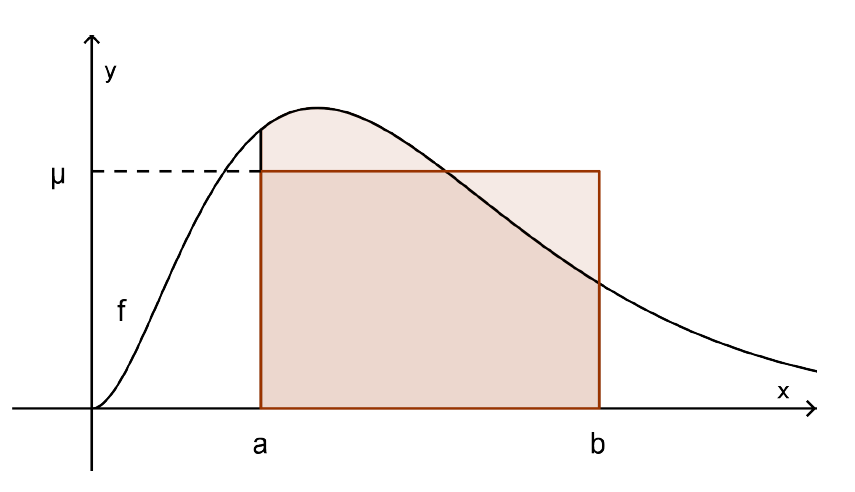
\includegraphics[width=0.4\linewidth]{Mittelwert_Grafik.png}
    \end{center}
  Definition des Mittelwert \(\mu\) der Funktion \(f(x)\) auf \([a,b]\): Höhe des Rechtecks, das
  \itemize
    \item eine Grundlinie der Länge \(b-a\) hat
    \item der Flächeninhalt des Rechteks der Fläche unter der Kurve \(f(x)\) im Intervall \([a,b]\) entspricht
	\[\mu = \frac{1}{b-a}\int_a^b{f(x)\mathrm{d}x} \]
\end{theorem}


\begin{theorem}{Schwerpunkt ebener Fläche}\\
  \begin{center}
  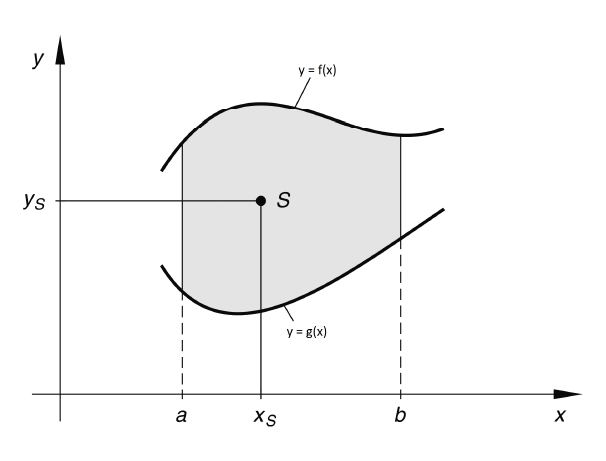
\includegraphics[width=0.4\linewidth]{Schwerpunkt_Beispiel.png}
  \end{center}
Schwerpunkt \(S=(x_s;y_s)\) einer ebenen Fläche mit Flächeninhalt A, eingegrenzt von Kurven \(y=f(x)\) und \(y=g(x)\)
sowie den Geraden \(x=a\) und \(x=b\):
\[xs = \frac{1}{A}\int_a^b{x\cdot(f(x)-g(x))\mathrm{d}x} \]
\[ys = \frac{1}{2A}\int_a^b{x\cdot(f(x)^2-g(x)^2)\mathrm{d}x} \]
Berechnen von \(A\) ebenfalls durch ein Integral:
\[A=\int_a^b{f(x)-g(x)\mathrm{d}x} \]
\end{theorem}
\begin{theorem}{Schwerpunkt Rotationskörper}\\
    Die x-Koordinate des Schwerpunkts \(S=(x_s;0;0) \) eines Rotationskörpers mit Volumen \(V\), geformt durch Rotation
    von \(y=f(x)\) zwischen \([a,b]\) um x-Achse mit \(a<b\) und \(f(x) \ge 0 \) für alle \(a \le x \le b \):
    \[x_s = \frac{\pi}{V}\int_a^b{x\cdot f(x)^2\mathrm{d}x} \]
\end{theorem}

\begin{formula}{Rotationsvolumen}
    $V = \pi \int_a^b{(f(x))^2\mathrm{d}x} $
\end{formula}
\begin{formula}{Bogenlänge}
    $L=\int_a^b{\sqrt{1+(f'(x))^2}\mathrm{d}x} $
\end{formula}
\begin{formula}{Mantelfläche}
    $M=2\pi \int_a^b{f(x)\cdot \sqrt{1+(f'(x))^2}\mathrm{d}x}$
\end{formula}

\raggedcolumns


\subsection{Uneigentliche Integrale}

\subsubsection{Uneigentliche Integrale erster Art}

\begin{KR}{Berechnung}
\begin{itemize}
	\item Rechnen mit endlichem Intervall \([a,\lambda] \text{ mit } \lambda \ge a \) anstelle von unendlichem
		Integral \([a,\infty) \)
		\[I(\lambda)=\int_a^{\lambda}{f(x)\mathrm{d}x} \]
	\item Das unendliche Intervall \([a,\infty) \) ergit sich aus \(\lim_{\lambda \rightarrow
		\infty}I(\lambda) \):
		\[I=\int_a^{\infty}{f(x)\mathrm{d}x}=\underset{\lambda \rightarrow \infty}{\lim}I(\lambda)=
		\underset{\lambda \rightarrow \infty}{\lim}(\int_a^{\lambda}{f(x)\mathrm{d}x}) \]
    \item Falls Grenzwert \(\underset{\lambda \rightarrow -\infty}{\lim}\) existiert, heisst das uneigentliche
        Integral \(\displaystyle\int_{a}^\infty {f(x)\mathrm{d}x}\) \(\bold{konvergent}\), andernfalls 
        \(\bold{divergent}\)
\end{itemize}
\end{KR}


\begin{KR}{Beidseitig unendliche Integrale}
\begin{itemize}
	\item Uneigentliche Integrale mit beidseitig unendlichen Integrationsinvervall:
		\[I=\int_{-\infty}^{\infty}{f(x)\mathrm{d}x}\]
	\item Einfügen einer künslichen Zwischengrenze \(c \in \mathbb{R}\\\text{typischerweise}\:c=0 \)
		\[\int_{-\infty}^{\infty}{f(x)\mathrm{d}x}=\int_{-\infty}^{c}{f(x)\mathrm{d}x}+\int_c^{\infty}
		{f(x)\mathrm{d}x} \]
	\item Beide Teilintegrale wie oben berechnen
	\item Das integral heisst \(\bold{konvergent}\) falls beide Teilintegrale konvergent sind.
\end{itemize}
\end{KR}

\subsubsection{Uneigentliche Integrale zweiter Art}
	\begin{definition}{Definition}\\
		Uneigentlich Integrale auf Interval \([a,b]\) mit einem Pol von \(f(x)\) bei \(x=a\) heisst,
		\(f(a) \rightarrow \infty\), und Stetigkeit auf \((a,b]\)
  \end{definition}
  \begin{KR}{Berechnung}
	  \begin{itemize}
	  	
\item Statt über \([a,b]\) integrieren, integrieren über \(a+\epsilon,b\) für beliebige \(\epsilon>0\):
	\[I(\epsilon)=\int_{a+\epsilon}^b{f(x)\mathrm{d}x}\]
\item Das Integral über \([a,b]\) ergibt sich aus \(\lim_{\epsilon \rightarrow 0}I(\epsilon)\):
	\[I=\int_a^b{f(x)\mathrm{d}x}=\underset{\epsilon \rightarrow 0}{\lim}I(\epsilon)=\underset{\epsilon \rightarrow
	0}{\lim}(\int_{a+\epsilon}^b{f(x)\mathrm{d}x}) \]
\item Das Integral heisst \(\bold{konvergent}\), falls der Limes \(\lim_{\epsilon \rightarrow 0}I(\epsilon)\) existiert.
\item Diese spezielle Variante ist nötig, weil beim Integralrechnen der Integral auf dem ganzen Intervall stetig sein
	muss. Dies ist nicht der Fall wen ein Pol existiert.
\end{itemize}
  \end{KR}


  \begin{formula}{Integraltabelle}\\
    \resizebox*{1.02\linewidth}{!}{
	\def\arraystretch{1.7}
	\begin{tabular}{c|c|c}
	    Ableitung | f'(x)                          & Funktion | f(x)                          & Integral | F(x)                       \\
        \hline
	    \(0\)                                      & \(C\)                                    & \(x+C\)                               \\
        \hline
        \(1\)                                      & \(x\)                                    & \(\frac{1}{2}x^2+C\)                  \\
        \hline
        \(-\frac{1}{x^2}\)                         & \(\frac{1}{x}\)                          & \(\ln|x|+C\)                          \\
        \hline
        \(ax^{a-1}\)                               & \(x^a \: with \: a \: \in \: \mathbb{R}\) & \(\frac{x^{a+1}}{a+1}+C\)             \\
        \hline
        $x^{x} \cdot(1+\ln x) \quad x>0$          & $x^{x}$                                  &   \\
        \hline
        $(x^{x})^{x}(x+2 x \ln (x)) \quad x>0$ & $x^{(x^{x})}$         &  \\
        \hline  
        
        $\frac{1}{2\sqrt{x}}$                     & $\sqrt{x}$                               &  $\frac{2}{3}x^{\frac{3}{2}}$         \\
        \hline
        $\frac{1}{n} x^{\frac{1}{n}-1}$           & $\sqrt[n]{x}$                            & $\frac{n}{n+1} x^{\frac{1}{n}+1}$     \\
        \hline

        \(\ln(a)\cdot a^x\)                       & \(a^x\)                                  & \(\frac{a^x}{\ln(a)}+C\)              \\
        \hline
        $a^{b x} \cdot c \ln a$                   & $a^{b x}$                                & $\frac{1}{b \ln a} a^{b x}$             \\
        \hline
        \(e^x\)                                   & \(e^x\)                                  & \(e^x+C\)                             \\
        \hline
        \(\frac{1}{x}\)                           & \(\ln(x)\)                               & \(x\ln(x)-x+C\)                       \\
        \hline
        \(\frac{1}{x\ln(a)}\)                     & \(\log_a(x)\)                            & \(x\log_a(x)-\frac{x}{\ln(a)}+C\)     \\
        \hline
        \(\cos(x)\)                                & \(\sin(x)\)                              & \(-\cos(x)+C\)                        \\
        \hline
        \(-\sin(x)\)                               & \(\cos(x)\)                              & \(\sin(x)+C\)                         \\
        \hline
        \(1+\tan^2{(x)=\frac{1}{\cos^2{(x)}}}\)    & \(\tan(x)\)                              & \(-\ln|\cos(x)|+C\)                   \\
        \hline
        \(-1-\cot^2{(x)}=-\frac{1}{\sin^2{(x)}}\)  & \(\cot(x)\)                              & \(\ln(\sin(x))+C\)                    \\
        \hline
        \(\frac{1}{\sqrt{1-x^2}}\)                & \(\arcsin(x)\)                           & \(x\arcsin(x)+\sqrt{1-x^2}+C\)        \\
        \hline
        \(-\frac{1}{\sqrt{1-x^2}}\)               & \(\arccos(x)\)                           & \(x\arccos(x)-\sqrt{1-x^2}+C\)        \\
        \hline
        \(\frac{1}{1+x^2}\)                       & \(\arctan(x)\)                           & \(x\arctan(x)-\frac{1}{2}\ln(1+x^2)+C\)\\
        %add more here
        \hline
        $\sin ^{2}(x)$                            & $\frac{1}{2}(x-\sin (x) \cos (x))$       & $\sin (x) \cos (x) + C$                   \\
        \hline
        $\cos ^{2}(x)$                            & $\frac{1}{2}(x+\sin (x) \cos (x))$       & $\cos (x) \sin (x) + C$                   \\ 
        \hline
        $\tan ^{2}(x)$                            & $\tan (x)-x$                             & $\tan (x) + C$                            \\
        \hline
        $\cot ^{2}(x)$                            & $-\cot (x)-x$                            & $\cot (x) + C$                            \\
        \hline
        $\frac{f'(x)}{f(x)}$                      & $\ln |f(x)|$                             & $x \cdot(\ln |x|-1) + C$                 \\
        \hline
        $\frac{1}{x}(\ln x)^{n}$                  & $\frac{1}{n+1}(\ln x)^{n+1} \quad n \neq-1$ & $\frac{1}{2 n}(\ln x^{n})^{2} \quad n \neq 0 + C$ \\
        \hline
        $\frac{1}{x \ln x}$                       & $\ln |\ln x| \quad x>0, x \neq 1$        & $\frac{1}{b \ln a} a^{b x} + C$           \\
        \hline
        $x \cdot e^{c x}$                         & $\frac{c x-1}{c^{2}} \cdot e^{c x}$      & $\frac{x^{n+1}}{n+1}(\ln x-\frac{1}{n+1}) \quad n \neq-1 + C$ \\
        \hline
        $x^{n} \ln x$                             & $\ln (\cosh (x))$                        & $\ln |f(x)| + C$                          \\
        \hline
        $\sin (x) \cos (x)$                       & $\frac{\sin^2(x)}{2} $                &\\
        \hline
        $\frac{-f^{\prime}(x)}{(f(x))^{2}}$       & $\frac{1}{f(x)}$                         & \\
        \hline
        $(a x+b)^{n}$                             & $\frac{1}{a \cdot(n+1)}(a x+b)^{n+1}$   & \\
        \hline
	\end{tabular}
    }
\end{formula}

\begin{KR}{Trick Gerade/Ungerade bei Integralen}\\
    Für ungerade Funktionen gilt $\int_{-a}^{+a} f(x) \dif x = 0$.
    \begin{itemize}
        \item Summe/Komposition: ungerade und ungerade $\rightarrow$ ungerade
        \item Produkt/Quotient: ungerade und gerade $\rightarrow$ ungerade
        \item Ableitung: gerade $\longrightarrow$ ungerade
    \end{itemize}
    Bsp ungerade: $f(x)$ = $-x$, $x$, $sin(x)$, $tan(x)$, Polynomfunktionen mit ungeradem Exponent\\
    gerade: $1$, $x^2$, $cos(x)$, $sec(x)$, Polynomf. mit geradem Exponent\\
    gerade und ungerade!! $f(x) = 0$
\end{KR}

\section{Differentialrechnung}




   

\subsubsection{Differentialquotient und Ableitung}


\begin{definition}{Sekanten-Steigung und Differentialquotient}
    $$\frac{\Delta f}{\Delta \mathrm{x}}=\frac{f(x_{0}+h)-f(x_{0})}{h}$$
\end{definition}

\begin{formula}{Tangentengleichung}
    $
    y=f^{\prime}(x_{0}) \cdot(x-x_{0})+f(x_{0})
    $
\end{formula}

\begin{definition}{Differenzierbarkeit}
    $f$ ist in $x_0$ \emph{differenzierbar}, falls der Grenzwert $\lim_{x \to x_0} \frac{f(x) -f(x_0)}{x -x_0}$ für alle 
    existiert.\\
    Den Grenzwert selbst bezeichnet man als Ableitung $f'(x)$ 
    \tcblower 
    \small
    Vereinfacht: Eine Funktion ist differenzierbar, falls die Kurve keine Knicke macht.
\end{definition}



\begin{definition}{Stetige Differenzierbarkeit}
	Eine Funktion ist stetig differenzierbar, wenn sie differenzierbar ist und ihre Ableitungsfunktion stetig ist.
\end{definition}


\begin{definition}{n-fache Differenzierbarkeit}
	\begin{enumerate}
		\item Für $n \geq 2$ ist $f$ \emph{$n$-mal differenzierbar} in $D$ falls $f^{n-1}$ in $D$ differenzierbar ist. Dann ist $f^{(n)} \coloneqq (f^{(n-1)})'$ 
		\item Die Funktion $f$ ist \emph{$n$-mal stetig differenzierbar} in $D$, falls sie $n$-mal differenzierbar ist und falls $f^{(n)}$ in $D$ stetig ist.
		\item Die Funktion $f$ ist in $D$ \emph{glatt}, falls sie $\forall n \geq 1$, $n$-mal differenzierbar ist. 
	\end{enumerate}
\end{definition}


\begin{itemize}
	\item $\exp$, $\sin$, $\cos$, $\sinh$, $\cosh$, $\tanh$ sind glatt auf $\R$
	\item Alle Polynome sind auf ganz $\R$ glatt
	\item $\ln : ]0, + \infty[ \to \R$ ist glatt
\end{itemize}


\begin{concept}{Ableitungsregeln}
    Seien $f,g: D \to \R$  differenzierbar. Dann gelten:
    \begin{itemize}
        \item Summe/Differenz: $(f + g)'(x) = f'(x) + g'(x)$
        \item Faktor: $f(x)=a\cdot g(x) \rightarrow f'(x)=a \cdot g'(x) $
        \item Produkt: $(f \cdot g)'(x) = f'(x)g(x) + f(x)g'(x)$
        \item Quotient: $(\frac{f}{g})'(x) = \frac{f'(x) g(x) - f(x) g'(x)}{g(x)^2}$
        \item Kettenregel: $(g \circ f)' (x) = g'(f(x)) f'(x)$
        \item Umkehrfunktion: $(f^{-1})'(y_0) = \frac{1}{f'(x)}$
        \item Potenz/Logarithmus 1: 
        $(a^{f(x)})' = ln(a) \cdot a^{f(x)} \cdot f'(x)$

        \resizebox{\linewidth}{!}{
            $(f(x)^{g(x)})' = f(x)^{g(x)} \cdot (ln(f(x)) \cdot g(x))' =  f(x)^{g(x)} \cdot (ln(f(x)) \cdot g(x) \cdot \frac{f'(x)}{f(x)})$
            }
    \end{itemize}
    Bem. Für gerade $k$ gilt $\cosh (x)^{(k)}=\cosh (x)$ und für ungerade $k$ gilt $\cosh (x)^{(k)}=\sinh (x)$, analoges gilt für $\sinh$.
\end{concept}

 \begin{KR}{Differentialrechnung Tricks}
        \begin{itemize}
      \item Überall differenzierbar: Einheitliche Tangente (Ableitung 0 setzen) und dh: Grenzwerte müssen denselben Wert ergeben
      \item Zwei Funktionskurven berühren sich (aww): bedeutet dass sie an Stelle x0 gleichen Funktionswert und gleiche Ableitung haben
      \item Tangente bestimmen (Linearisierung): $f(x_{0})+f^{\prime}(x_{0})(x-x_{0})$
    \end{itemize}
    \end{KR}

\begin{formula}{Grundfunktionen der Ableitung}
    \begin{itemize}
        \item Potenz 
    \end{itemize}
    \vspace{-3mm}
    $$f(x)=x^{n} \quad f^{\prime}(x)=n \cdot x^{n-1}$$
    \begin{itemize}
      \item Exponent
    \end{itemize}
    \vspace{-3mm}
    $$
    \begin{array}{ll}
    f(x)=a^{x} & f^{\prime}(x)=a^{x} \cdot \ln (a) \\
    f(x)=e^{x} & f^{\prime}(x)=e^{x}
    \end{array}
    $$
    
    \begin{itemize}
      \item Logarithmus
    \end{itemize}
    \vspace{-3mm}
    $$
    \begin{array}{ll}
    f(x)=\ln (x) & f^{\prime}(x)=\frac{1}{x} \\
    f(x)=\log _{a}(x) & f^{\prime}(x)=\frac{1}{\ln (a) \cdot x}
    \end{array}
    $$
\end{formula}


\begin{formula}{Ableitungen von geometrischen Funktionen}
    $$
    \arctan ^{\prime}(x) =\frac{1}{1+x^{2}}, 
    \arcsin ^{\prime}(x) =\frac{1}{\sqrt{1-x^{2}}}, 
    \arccos ^{\prime}(x) =\frac{1}{\sqrt{1+x^{2}}}
    $$

    $$
    \begin{array}{ll}
    f(x)=\tan (x) & f^{\prime}(x)=1+\tan ^{2}(x)=\frac{1}{\cos ^{2}(x)} \\
    f(x)=\cot (x) & f^{\prime}(x)=-1-\cot ^{2}(x)=-\frac{1}{\sin ^{2}(x)}
    \end{array}
    $$
\end{formula}

\begin{definition}[breakable]{Monotonie}\\
    Sei $y=f(x)$ eine differenzierbare Funktion in $D$ mit $x_{0} \in D$.
    \begin{itemize}
        \item $f'( x_{0}) = 0$ $ \Rightarrow$   $f$ konstant, bzw. horizontale Tangente
        \item $f'( x_{0}) > 0 $ $ \Rightarrow$  $f$  streng monoton wachsend.
        \item $f'( x_{0}) < 0 $ $ \Rightarrow$ $f$ streng monoton fallend.
    \end{itemize}
\end{definition}
\begin{theorem}{Krümmung}\\
    Zusammenhang zwischen 2. Ableitung und Krümmung:
    \begin{itemize}
      \item $f^{\prime \prime}(x_{0})>0$ Konvex (Nach links/oben gekrümmt)
      \item $f^{\prime \prime}(x_{0})<0$ Konkav (Nach rechts/unten gekrümmt)
      \item $f^{\prime \prime}(x_{0})=0$ Keine eindeutige Krümmung
    \end{itemize}
    Bmk: Die Summe zweier konvexer Funktionen ist konvex. (konkav analog)
\end{theorem}

\begin{KR}{Vorgehen Wende- und Sattelpunkte}
    \begin{enumerate}
  \item Erste und zweite Ableitung

  \item Wendepunkt bestimmen

\end{enumerate}

\begin{itemize}
  \item $f^{\prime \prime}(x_{0})=0 \rightarrow x_{0}$
  \item $f^{(3)}(x_{0}) \neq 0$
\end{itemize}

\begin{enumerate}
  \setcounter{enumi}{2}
  \item Sattelpunkte bestimmen
\end{enumerate}

\begin{itemize}
  \item $f^{\prime}(x_{0})=0$
  \item $f^{\prime \prime}(x_{0})=0$
  \item ...
  \item $f^{(n)}(x_{0}) \neq 0$
  \item Gerade $\rightarrow$ relatives Extremum
  \item Ungerade $\rightarrow$ Sattelpunkt
\end{itemize}

\begin{enumerate}
  \setcounter{enumi}{3}
  \item $x_{0}$ in ursprüngliche Gleichung einsetzen
\end{enumerate}
\end{KR}

\begin{KR}{Berechnung Wendetangente}
    Ermittlung durch Lösen der Gleichung $f^{\prime \prime}(x)=0 \rightarrow x_{0}$.\\
    Bedingungen:\\
    Sei $y=f(x)$ dreimal differenzierbar

\begin{itemize}
  \item $f^{\prime \prime}(x_{0})=0$
  \item $f^{(3)}(x_{0}) \neq 0 \quad \rightarrow$ Wendepunkt
  \item Falls zusätzlich $f^{\prime}(x_{0})=0 \quad \rightarrow$ Sattelpunkt
\end{itemize}
    
\end{KR}

\begin{KR}{Vorgehen relative Extrema} von $f(x) = y$:
    \begin{enumerate}
	\item Bestimme $f'(x)$ (Erste Ableitung)
	\item Bestimme NST von $f'(x)$\\
		$f'(x) = 0$ $ \Rightarrow$ $x$ lokales Extremum
	\item Bestimme $f''(x)$ (Zweite Ableitung)
		\begin{itemize}
			\item $f''(x) = 0$ $ \Rightarrow$ siehe Vorgehen Wende- und Sattelpunkte
			\item $f''(x) < 0$ $ \Rightarrow$ relatives Maximum
			\item $f''(x) > 0$ $ \Rightarrow$ relatives Minimum
		\end{itemize}
    \item In Gleichung f(x) = y einsetzen
        \begin{itemize}
            \item Hochpunkt/Tiefpunkt = $P(x, y)$
        \end{itemize}
\end{enumerate}
\end{KR}















































    \raggedcolumns
    \pagebreak
    

\section{Vektorgeometrie}

\begin{definition}{Vektor}
    Objekt, das Betrag und Richtung hat.
    \begin{itemize}
        \item $\overrightarrow{0} = $ Nullvektor (Betrag = 0, einziger Vektor ohne Richtung)
        \item $\overrightarrow{e} = $ Einheitsvektor (Betrag = 1), evtl. mit Index $\vec{e_a}$
        \item $\vec{PQ}=$ Vektor, der den Punkt $P$ in $Q$ verschiebt
        \item $\vec{a} = \vec{b} \Leftrightarrow \abs{\vec{a}} = \abs{\vec{b}}$ und $\vec{a} \parallel \vec{b}$ (selber Betrag und Richtung)
    \end{itemize}
    Es wird zwischen \textit{Orts-} und \textit{Richtungsvektoren} unterschieden.
\end{definition}

\begin{minipage}{0.6\linewidth}
    \begin{definition}{Gegenvektor}
        $-\vec{a}$ ist parallel zu $\vec{a}$, hat denselben Betrag,
        aber entgegengesetzte Richtung. 
    \end{definition}
    \end{minipage}
    \begin{minipage}{0.25\linewidth}
        {\small
        $$-\overrightarrow{a} = \begin{pmatrix}
            -a_x \\
            -a_y
            \end{pmatrix}$$}
    \end{minipage}
    \begin{minipage}{0.13\linewidth}
        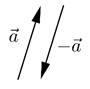
\includegraphics[width=0.8\linewidth]{vec-gegen.png}
    \end{minipage}

\begin{definition}{Länge/Betrag eines Vektors}
    $\abs{\vec{a}}=\sqrt{a_1^2+a_2^2+\cdots+a_n^2}$
\end{definition}

\begin{formula}{Einheitsvektor/Normierung}
    {\large
    $\vec{e_a}=\frac{1}{a}\cdot\vec{a} \quad = \quad \frac{\overrightarrow{a}}{|\overrightarrow{a}|}$}

    Der Vektor $\vec{e_a}$ wird als \textbf{Einheitsvektor oder auch normiert} bezeichnet 
    und der Übergang von $\vec{a}$ nach $\vec{e_a}$ heisst \textbf{Normierung}.
\end{formula}



\begin{definition}{Orthogonal (Senkrecht)} $\overrightarrow{a} \cdot \overrightarrow{b} = 0 \rightarrow \text{ orthogonal}$

    $\vec{a}$ und $\vec{b}$ sind orthogonal, wenn der Winkel zwischen ihnen 90° beträgt
\end{definition}

\begin{definition}{Normalenvektor}
    Ein Normalenvektor, der orthogonal zu einer Ebene $E$ ist, heisst \textit{Normalenvektor} von $E$.
    Eine Koordinatendarstellung einer Ebene $E$ heisst normiert, wenn gilt: $\vec{n}=1$.
\end{definition}



\raggedcolumns

\paragraph*{Rechnen mit Vektoren}

\begin{minipage}{0.5\linewidth}
    \begin{formula}{Vektoraddition}\\
        $\overrightarrow{a} + \overrightarrow{b} = \begin{pmatrix} a_x + b_x\\ a_y + b_y \end{pmatrix}$
    \end{formula}
\end{minipage}
\begin{minipage}{0.5\linewidth}
\begin{formula}{Skalarmultiplikation}\\
    $\lambda \cdot \overrightarrow{a} = \begin{pmatrix}
    \lambda \cdot a_x \\
    \lambda \cdot a_y
    \end{pmatrix}$
\end{formula}
\end{minipage}

\raggedcolumns

\begin{formula}{Skalarprodukt} 
    $\overrightarrow{a} \cdot \overrightarrow{b} = a_x \cdot b_x + a_y \cdot b_y = |\overrightarrow{a}| \cdot |\overrightarrow{b}| \cdot \cos(\varphi)$
\end{formula}

\begin{formula}{Winkelberechnung} {\small $\varphi$ = Winkel zwischen $\vec{a}$ und $\vec{b}$ ($0\le\phi\le\pi$)}
    $$\cos(\varphi) = \frac{\overrightarrow{a} \cdot \overrightarrow{b}}{|\overrightarrow{a}| \cdot |\overrightarrow{b}|} = \frac{a_x b_x + a_y b_y}{\sqrt{a_x^2 + a_y^2} \cdot \sqrt{b_x^2 + b_y^2}  } $$
\end{formula}


\begin{minipage}{0.55\linewidth}
\begin{concept}{Winkel und Skalarprodukt}\\
    Seien $\vec{a}$ und $\vec{b}$ zwei Vektoren und $\varphi$ der eingeschlossene Winkel, 
    $0\leq\varphi\leq\pi$, dann gilt:
\end{concept}
\end{minipage}
\begin{minipage}{0.35\linewidth}
    $\varphi<\frac{\pi}{2},\, \text{ wenn } \vec{a}\cdot\vec{b} > 0 \\  
    \varphi>\frac{\pi}{2},\, \text{ wenn } \vec{a}\cdot\vec{b} < 0 \\   
    \varphi=\frac{\pi}{2},\, \text{ wenn } \vec{a}\cdot\vec{b} = 0 $
\end{minipage}

\begin{theorem}{Eigenschaften des Skalarprodukts}\\ Für beliebige Vektoren $\vec{a}$, $\vec{b}$, $\vec{c}$ und Skalaren $\lambda\in\R$ gilt:
    \begin{itemize}
        \item $\vec{a}\cdot\vec{a}=\abs{\vec{a}}^2$
        \item $(-\lambda)\cdot\vec{a}=-(\lambda\cdot\vec{a})=\lambda\cdot(-\vec{a})$
        \item Kommutativ-Gesetz: $\vec{a}\cdot\vec{b}=\vec{b}\cdot\vec{a}$
        \item Distributiv-Gesetze: $\vec{a}\cdot(\vec{b}+\vec{c})=\vec{a}\cdot\vec{b}+\vec{a}\cdot\vec{c}$ und $(\vec{a}+\vec{a})\cdot\vec{c}=\vec{a}\cdot\vec{c}+\vec{b}\cdot\vec{c}$
        \item Gemischtes Assoziativ-Gesetz: $\lambda\cdot(\vec{a}\cdot\vec{b})=(\lambda\cdot\vec{a})\cdot\vec{b}=\vec{a}\cdot(\lambda\cdot\vec{b})$
    \end{itemize} 
\end{theorem}

\begin{minipage}{0.8\linewidth}
\begin{formula}{Kreuzprodukt} {\small $\overrightarrow{a} \times \overrightarrow{b}$ ist orthogonal zu $\overrightarrow{a}$ und $\overrightarrow{b}$
        $$\overrightarrow{a} \times \overrightarrow{b} = (\begin{array}{ccc}
            a_y \cdot b_z &-& a_z \cdot b_y \\
            a_z \cdot b_x &-& a_x \cdot b_z \\
            a_x \cdot b_y &-& a_y \cdot b_x
            \end{array})$$
    \vspace{2mm}
    $|\overrightarrow{a} \times \overrightarrow{b}| = |\overrightarrow{a}| \cdot |\overrightarrow{b}| \cdot \sin(\varphi) 
        \quad \quad \quad \overrightarrow{a} \times \overrightarrow{b} \neq \overrightarrow{b} \times \overrightarrow{a}$
    
        \vspace{1mm}

        Für $\R^2$ gilt: $\overrightarrow{a} \times \overrightarrow{b} = a_x \cdot b_y - a_y \cdot b_x$
        }
\end{formula}
\end{minipage}
\begin{minipage}{0.19\linewidth}
    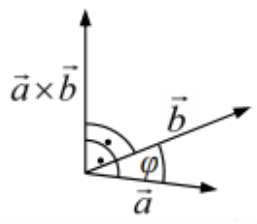
\includegraphics[width=1\linewidth]{vektorprodukt.png}
\end{minipage}  

\begin{theorem}{Eigenschaften des Kreuzprodukts} auch genannt Vektorprodukt\\
    Für beliebige Vektoren $\vec{a}$, $\vec{b}$, $\vec{c}$ und Skalaren $\lambda\in\R$ gilt:
    \begin{itemize}
        \item $\vec{a}\times\vec{a}=\vec{0}$
        \item Antikommutativ-Gesetz: $\vec{a}\times\vec{b}=-(\vec{b}\times\vec{a})$
        \item Distributiv-Gesetz: $\vec{a}\times(\vec{b}+\vec{c})=\vec{a}\times\vec{b}+\vec{a}\times\vec{c}$
        \item Gemischtes Assoziativ-Gesetz:
            $\lambda\cdot(\vec{a}\times\vec{b})=(\lambda\cdot\vec{a})\times\vec{b}=\vec{a}\times(\lambda\cdot\vec{b})$ 
    \end{itemize}
    \textcolor{pink}{$\vec{a}\times(\vec{b}\times\vec{c})\ne(\vec{a}\times\vec{b})\times\vec{c}$!!}
\end{theorem}

\begin{formula}{Fläche des aufgespannten Parallelogramms} = $\vec{a}\times\vec{b}$\\
    \begin{minipage}{0.6\linewidth}
    $$h = |\overrightarrow{b}| \cdot \sin(\varphi)$$
    $$A = |\overrightarrow{a}| \cdot h = |\overrightarrow{a} \times \overrightarrow{b}| = |\overrightarrow{a}| \cdot |\overrightarrow{b}| \cdot \sin(\varphi)$$
    \end{minipage}
    \hspace{3mm}
    \begin{minipage}{0.35\linewidth}
        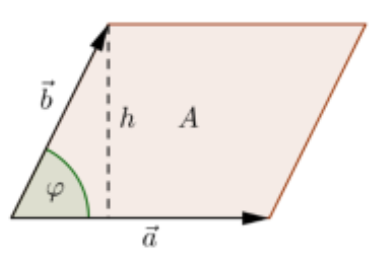
\includegraphics[width=0.7\linewidth]{parallelogramm.png}
    \end{minipage}
\end{formula}



\begin{minipage}{0.7\linewidth}
    \begin{formula}{Orthogonal Projektion}von $\overrightarrow{b}$ auf $\overrightarrow{a}$
            $$\vec{b}_a=\frac{\vec{a}\cdot\vec{b}}{\abs{\vec{a}}^2}\cdot\vec{a}   
            \text{ und }
            \abs{\vec{b}}_a=\frac{\abs{\vec{a}\cdot\vec{b}}}{\abs{\vec{a}}}  $$
    \end{formula}
\end{minipage}
    \begin{minipage}{0.25\linewidth}
        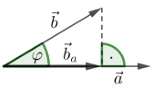
\includegraphics[width=0.9\linewidth]{vec-proj.png}
    \end{minipage}
    \begin{remark}
        Die erste Formel gilt für $0<\varphi\leq\frac{\pi}{2}$,
        die zweite für $\frac{\pi}{2}<\varphi\leq\pi$
    \end{remark}


\paragraph*{Lineare Abhängigkeit und Komponentendarstellung}

\begin{definition}{Linearkombination (LK)}
    $\lambda_1\cdot\vec{a_1}+\lambda_2\cdot\vec{a_2}+\ldots+\lambda_n\cdot\vec{a_n}$
    
    \vspace*{2mm}

    mit $\lambda_n\in R$ heisst \textit{Linearkombination} der Vektoren $\vec{a_1},\ldots,\vec{a_n}$.
\end{definition}

\begin{definition}{Lineare Abhängigkeit}
    $\overrightarrow{a_{1}}, \overrightarrow{a_{2}}, \ldots, \overrightarrow{a_{k}}$ sind linear unabhängig, wenn:
    \vspace*{1mm}
    \begin{itemize}
    \item $\lambda_{1} \cdot \overrightarrow{a_{1}}+\lambda_{2} \cdot \overrightarrow{a_{2}}+\cdots+\lambda_{k} \cdot \overrightarrow{a_{k}} \neq \overrightarrow{0}(\lambda>0 \wedge \lambda \in \mathbb{R})$
    \item $0 \cdot \overrightarrow{a_{1}}+0 \cdot \overrightarrow{a_{2}}+\cdots+0 \cdot \overrightarrow{a_{k}}$ als einzige LK $\overrightarrow{0}$ ergibt
\end{itemize}
\end{definition}

\begin{definition}{Komponentendarstellung} $\vec{a}=a_1\cdot\vec{e}_1+\cdots+a_n\cdot\vec{e}_n=
    \begin{psmallmatrix}
        a_1\\\scalebox{0.5}{\vdots}\\a_n
    \end{psmallmatrix}$

    $\exists a_1, ... a_n \in \R$ (Komponente), so dass
    jeder Vektor $\vec{a}$ \\als LK von $\vec{e}_1,...\vec{e}_n$
    eindeutig dargestellt werden kann. 
\end{definition}

\begin{definition}{Ortsvektor}
    $\vec{r}(P)=\overrightarrow{OP}=x_1\cdot\vec{e}_1+...+x_n\cdot\vec{e}_n =
    \begin{psmallmatrix}
        x_1\\\scalebox{0.5}{\vdots}\\x_n
    \end{psmallmatrix}$
    
    Zu jedem Punkt $P$ des Vektorraums definiert! Ortsvektoren sind im Ursprung $O$ angeheftet, wie jeder Vektor LK 
    von $\vec{e_1}, ... \vec{e_n}$ und lassen sich in Komponentenschreibweise darstellen:
\end{definition}

\begin{minipage}{0.6\linewidth}
\begin{formula}{Komponentendarstellung von $\overrightarrow{OP}$}
    
    $\vec{r}(Q)=\vec{r}(P)+\overrightarrow{PQ}\\
    \Rightarrow \overrightarrow{PQ}=\vec{r}(Q)-\vec{r}(P)=\begin{pmatrix}
        x_Q-x_P\\
        y_Q-y_P\\
        \cdots-\cdots
    \end{pmatrix}$
\end{formula}
\end{minipage}
\begin{minipage}{0.38\linewidth}
    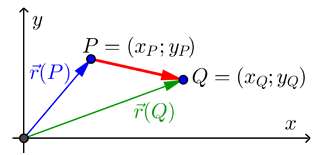
\includegraphics[width=\linewidth]{vec-komp-calc.png}
\end{minipage}


\raggedcolumns


\subsubsection*{Geraden und Ebenen}

\paragraph*{Kollinear und Komplanar}   

\begin{definition}{Kollinear} $\vec{a}$ und $\vec{b}$\\
    \begin{minipage}{0.8\linewidth}
    \begin{itemize}
        \item $\exists$ eine Gerade $g$, zu der beide parallel sind
        \item Spezialfall: Nullvektor ist zu jedem Vektor kollinear
        \item $\vec{a} \times \vec{b} = \vec{0}$ (Kreuzprodukt)
        \item $\vec{a}=\lambda\cdot\vec{b}$ (einer ist Vielfaches des anderen)
    \end{itemize}
    \end{minipage}
    \hspace{3mm}
    \begin{minipage}{0.1\linewidth}
        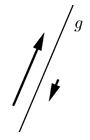
\includegraphics[width=1\linewidth]{vec-kollinear.png}
    \end{minipage}
\end{definition}

\begin{theorem}{Lage} von Geraden im Raum\\
    \vspace*{2mm}
    %make a table to show the different cases
    \begin{tabular}{c|c|c|}
        & Gemeinsame Punkte & keine gem. Punkte \\
        \hline
        Kollinear & Identisch & echt Parallel \\
        \hline
        nicht kollinear & Schneidend & Windschief \\
        \hline
    \end{tabular}
\end{theorem}

\begin{minipage}{0.8\linewidth}
\begin{definition}{Komplanar} $\vec{a}$, $\vec{b}$ und $\vec{c}$\\
    Es existiert eine Ebene $E$, zu der alle parallel sind.
\end{definition}
\end{minipage}
\begin{minipage}{0.15\linewidth}
    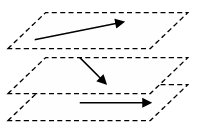
\includegraphics[width=\linewidth]{vec-komplanar.png}
\end{minipage}

\begin{minipage}{0.7\linewidth}
    \begin{theorem}{LK komplanarer Vektoren} $\vec{a}$, $\vec{b}$ und $\vec{c}$\\
        Wenn $\vec{a}$ und $\vec{b}$ nicht kollinear sind lässt sich $\vec{c}$ als Linearkombination von $\vec{a}$ und $\vec{b}$ mit $\lambda, \mu \in \R$ darstellen:
            {\large$\vec{c}=\lambda\cdot\vec{a}+\mu\cdot\vec{b}$}
    \end{theorem}
    \end{minipage}
    \begin{minipage}{0.25\linewidth}
        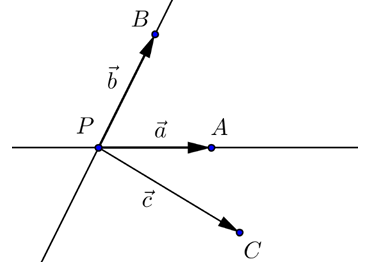
\includegraphics[width=\linewidth]{vec-kompl.png}
\end{minipage}

\begin{minipage}{0.7\linewidth}
    \begin{theorem}{LK nicht komplanarer Vektoren} $\vec{a}$, $\vec{b}$ und $\vec{c}$\\
        Jeder Vektor $\vec{d}$ im $\R^3$ lässt sich als Linearkombination von $\vec{a}$, $\vec{b}$ und $\vec{c}$ eindeutig darstellen:
            {\large$\vec{d}=\lambda\cdot\vec{a}+\mu\cdot\vec{b}+\nu\cdot\vec{c}$}
    \end{theorem}
    \end{minipage}
    \begin{minipage}{0.25\linewidth}
        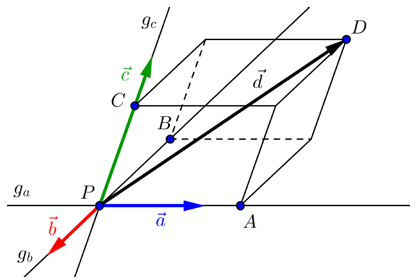
\includegraphics[width=\linewidth]{vec-nicht-kompl.png}
\end{minipage}

\paragraph{Darstellungsformen von Ebenen und Geraden}

\begin{minipage}{0.6\linewidth}
    \begin{definition}{Parameterdarstellung} einer Geraden
        $$\overrightarrow{r}(A) = \overrightarrow{r}(P) + \lambda \cdot \overrightarrow{PQ}$$
    
        {\small Der Punkt $P$ heisst \textit{Aufpunkt}, der Vektor $\overrightarrow{a} = \overrightarrow{PQ}$ heisst \textit{Richtungsvektor} von $g$.}
    \end{definition}
\end{minipage}
\begin{minipage}{0.4\linewidth}
    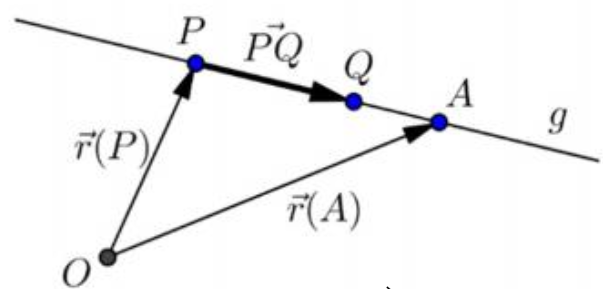
\includegraphics[width=1\linewidth]{gerade.png}\\
    $g: \overrightarrow{r}(P) + \lambda \cdot \overrightarrow{a}$
\end{minipage}


\begin{minipage}{0.6\linewidth}
\begin{definition}{Parameterdarstellung} einer Ebene
    $$E:\,\vec{r}(P)+\lambda\cdot\vec{a}+\mu\cdot\vec{b}\, (\lambda,\mu\in\R)$$
    $P$ = \textit{Aufpunkt}, $a=\overrightarrow{PQ}$ und 
    $\vec{b}=\overrightarrow{PR}$ sind \textit{Richtungsvektoren} von $E$.\\

    Parameterdarstellung nicht eindeutig!\\ Richtungsvektoren zwei beliebige
    Vektoren: \textit{parallel} zu $E$ und \textit{nicht kollinear}
\end{definition}
\end{minipage}
\begin{minipage}{0.4\linewidth}
    \begin{center}
    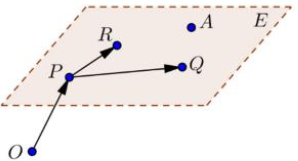
\includegraphics[width=0.8\linewidth]{ebene.png}
    \end{center}
    $\overrightarrow{PA}$, $\overrightarrow{PR}$, $\overrightarrow{PQ}$ komplanar\\

    $\overrightarrow{PA} = \lambda \cdot \overrightarrow{PR} + \mu \cdot \overrightarrow{PQ}$
\end{minipage}


\begin{definition}{Koordinatendarstellung} $a,b,c,d\in \R$
    $$E:\,ax+by+cz+d=0$$
    Bedeutung: die Ebene E besteht aus allen Punkten $P$, deren Koordinaten
    $x, y$ und $z$ diese Gleichung erfüllen.
    $\abs{d}$ = Abstand zum Ursprung, wenn Gleichung normiert
    (sonst $\frac{\vec{d}}{\vec{n}}$)
    {\small
    $$\vec{n} = \begin{pmatrix} a \\ b \\ c \end{pmatrix}, \quad
    \vec{n} \perp \begin{pmatrix} x \\ y \\ z \end{pmatrix}, \quad
    \begin{pmatrix} x \\ y \\ z \end{pmatrix} \cdot \begin{pmatrix} a \\ b \\ c \end{pmatrix} = 0$$
    }
\end{definition}

\paragraph*{Umrechnung von Parameter- und Koordinatendarstellung}

\begin{formula}{Umrechnung Parameterdarstellung zu Koordinatendarstellung}\\
    Berechnen über den Normalenvektor aus dem Kreuzprodukt der Richtungsvektoren,
    welches die Koeffizienten $a, b$ und $c$ liefert. 
    Der Aufpunkt wird über das Einsetzen eines Punktes der Ebene $E$ ermittelt.
    $$
        \vec{n}=\vec{a}\times\vec{b}=\begin{psmallmatrix}
            a\\b\\c
        \end{psmallmatrix}
    $$
\end{formula}

\begin{example2}{Parameterdarstellung $\rightarrow$ Koordinatendarstellung}
    $$E: \begin{psmallmatrix} 2 \\ 4 \\ 1 \end{psmallmatrix} + \lambda \cdot \begin{psmallmatrix} 1 \\ 3 \\ 1 \end{psmallmatrix} + \mu \cdot \begin{psmallmatrix} 2 \\ 2 \\ -4 \end{psmallmatrix}$$
    $$\vec{n} = \begin{psmallmatrix} 1 \\ 3 \\ 1 \end{psmallmatrix} \times \begin{psmallmatrix} 2 \\ 2 \\ -4 \end{psmallmatrix} = \begin{psmallmatrix} -12 -2 \\ 2 + 4 \\ 2 - 6 \end{psmallmatrix} = \begin{psmallmatrix} -14 \\ -6 \\ -4 \end{psmallmatrix}$$
    $$E: -14x - 6y - 4z + d = 0$$
    Aufpunkt einsetzen: $-14 \cdot 2 - 6 \cdot 4 - 4 \cdot 1 + d = 0 \Rightarrow d = 8$
\end{example2}

\begin{formula}{Umrechnung Koordinatendarstellung zu Parameterdarstellung}\\
    Um eine Koordinatendarstellung in eine Parameterdarstellung umzurechnen,
    werden drei Punkte berechnet.
    Einer dieser Punkte wird dann als aufpunkt gewählt und mit den restlichen
    werden Richtungsvektoren berechnet.
\end{formula}

\begin{example2}{Koordinatendarstellung $\rightarrow$ Parameterdarstellung}
    $$E: 2x + 7y - 4z + 1 = 0$$
    Punkte einsetzen: $(0|0|z), (1|0|z), (0|1|z)$\\
    \begin{minipage}{0.5\linewidth}
    \begin{itemize}
        \item $2 \cdot 0 + 7 \cdot 0 - 4 \cdot z + 1 = 0 \Rightarrow z = \frac{1}{4}$
        \item $2 \cdot 1 + 7 \cdot 0 - 4 \cdot z + 1 = 0 \Rightarrow z = \frac{3}{4}$
        \item $2 \cdot 0 + 7 \cdot 1 - 4 \cdot z + 1 = 0 \Rightarrow z = \frac{8}{4}$
    \end{itemize}
    \end{minipage}
    \hspace{2mm}
    \begin{minipage}{0.45\linewidth}
    $E: \begin{psmallmatrix} 0 \\ 0 \\ \frac{1}{4} \end{psmallmatrix} +
    \lambda \begin{psmallmatrix} 1 \\ 0 \\ \frac{2}{4} \end{psmallmatrix} +
    \mu \begin{psmallmatrix} 0 \\ 1 \\ \frac{7}{4} \end{psmallmatrix}$
    \end{minipage}
\end{example2}



\paragraph*{Abstände berechnen}


\begin{formula}{Abstand Punkt-Gerade}Gesucht ist der Fusspunkt $B\in g$\\
    Gegeben: Gerade $g=\vec{r}(P)+\lambda\cdot\vec{a}$ in Parameterform und Punkt $A$
    
    \begin{minipage}{0.59\linewidth}
        \begin{enumerate}
            \item Da $B\in g\Rightarrow \vec{r}(B)=\vec{r}(P)+\lambda_B\cdot\vec{a}$ 
            \item $\vec{BA}=\vec{r}(A)-\vec{r}(B)$
            \item $\vec{BA}\perp g\Rightarrow\vec{BA}\cdot\vec{a}=0$
            \item $l=\abs{\vec{BA}}$ ($\lambda_B$ in $\vec{BA}$ einsetzen)
        \end{enumerate}
    \end{minipage}
    \begin{minipage}{0.4\linewidth}
        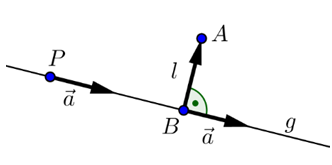
\includegraphics[width=1\linewidth]{vec-abstand-von-punkt.png}
    \end{minipage}

    Meist einfacher:
    $\vec{PA}=\vec{r}(A)-\vec{r}(P) \Rightarrow l=\frac{\abs{\vec{PA}\times\vec{a}}}{\abs{\vec{a}}}$   
\end{formula}

\begin{formula}{Abstand Punkt-Ebene} $l$ = Abstand von $A$ zu $E$\\
    \begin{minipage}{0.7\linewidth}
    Gegeben: Punkt $A=(x_A;y_A;z_A)$, Ebene $E$ mit der \textbf{normierten} 
    Koordinatendarstellung $E:\,ax+by+cz+d=0$
    \begin{center}
    $l=\abs{ax_A+by_A+cz_A+d}$
    \end{center}
    \end{minipage}
    \hspace{3mm}
    \begin{minipage}{0.2\linewidth}
        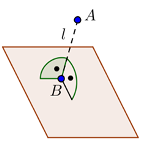
\includegraphics[width=1\linewidth]{vec-abstand-von-ebene.png}
    \end{minipage}

    \begin{minipage}{0.65\linewidth}
        \textbf{nicht normierte} Koordinatendarstellung:
    $$l=\frac{\abs{ax_A+by_A+cz_A+d}}{\abs{\vec{n}}}$$
    \end{minipage}
    \begin{minipage}{0.3\linewidth}
        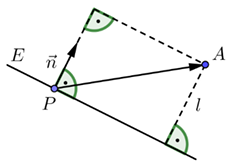
\includegraphics[width=0.9\linewidth]{vec-abstand-von-ebene2.png}
    \end{minipage}
\end{formula}


\section{Geometrische Transformationen}

\subsection{$\R^2$}

\begin{formula}{Streckung}\\
    \begin{minipage}{0.4\linewidth}
        \begin{itemize}
            \item in $x$-Richtung um $\lambda_1$
            \item in $y$-Richtung um $\lambda_2$
        \end{itemize}
    \end{minipage}
    \begin{minipage}{0.6\linewidth}
        $$\begin{pmatrix} x' \\ y' \end{pmatrix} = \begin{pmatrix} \lambda_1 & 0 \\ 0 & \lambda_2 \end{pmatrix} \cdot \begin{pmatrix} x \\ y \end{pmatrix}$$
    \end{minipage}
\end{formula}

\begin{formula}{Spiegelung}\\
    \begin{minipage}{0.45\linewidth}
        \begin{itemize}
            \item Gerade $g: ax + by = 0$
            \item mit $a^2 + b^2 = 1$
        \end{itemize}
    \end{minipage}
    \begin{minipage}{0.5\linewidth}
        $$\begin{pmatrix} 1 - 2a^2 & -2ab \\ -2ab & 1 - 2b^2 \end{pmatrix}$$
    \end{minipage}
\end{formula}

\begin{example}
    \begin{minipage}{0.5\linewidth}
        \begin{itemize}
            \item Gerade $g: x + 7y = 0$
            \item Normiert $g: \frac{1}{\sqrt{50}} x + \frac{7}{\sqrt{50}} y = 0$
        \end{itemize}
    \end{minipage}
    \begin{minipage}{0.45\linewidth}
        $$\frac{1}{50} \cdot \begin{pmatrix} 48 & -14 \\ -14 & -48 \end{pmatrix}$$
    \end{minipage}
\end{example}

\begin{formula}{Orthogonale Projektion}\\
    \begin{minipage}{0.5\linewidth}
    \begin{itemize}
        \item auf Gerade $g: ax + by = 0$
        \item mit $a^2 + b^2 = 1$
    \end{itemize}
    \end{minipage}
    \begin{minipage}{0.5\linewidth}
    $$\begin{pmatrix} 1 - a^2 & -ab \\ -ab & 1-b^2 \end{pmatrix}$$
    \end{minipage}
\end{formula}

\begin{example}
    \begin{minipage}{0.5\linewidth}
    \begin{itemize}
        \item Gerade $g: 2x -y = 0$
        \item Normiert $g: \frac{2}{\sqrt{5}} x - \frac{1}{\sqrt{5}} y = 0$ 
    \end{itemize}
    \end{minipage}
    \begin{minipage}{0.45\linewidth}
    $$\frac{1}{5} \cdot \begin{pmatrix} 1 & 2 \\ 2 & 4 \end{pmatrix}$$
    \end{minipage}
\end{example}

\begin{formula}{Rotation}\\
    \begin{minipage}{0.35\linewidth}
    \begin{itemize}
        \item um den Ursprung
        \item um Winkel $\alpha$
    \end{itemize}
    \end{minipage}
    \begin{minipage}{0.65\linewidth}
    $$\begin{pmatrix} x' \\ y' \end{pmatrix} = \begin{pmatrix} \cos(\alpha) & -\sin(\alpha) \\ \sin(\alpha) & \cos(\alpha) \end{pmatrix} \cdot \begin{pmatrix} x \\ y \end{pmatrix}$$
    \end{minipage}
\end{formula}

\begin{formula}{Scherung}\\
    \begin{minipage}{0.5\linewidth}
    \begin{itemize}
        \item in $x$-Richtung um $s_1$
        \item in $y$-Richtung um $s_2$
    \end{itemize}
    \end{minipage}
    \begin{minipage}{0.5\linewidth}
    $$\begin{pmatrix} x' \\ y' \end{pmatrix} = \begin{pmatrix} 1 & s_1 \\ s_2 & 1 \end{pmatrix} \cdot \begin{pmatrix} x \\ y \end{pmatrix}$$
    \end{minipage}
\end{formula}

\columnbreak

\subsection*{$\R^3$}

\begin{formula}{Zentrische Streckung}\\
    \begin{minipage}{0.4\linewidth}
    \begin{itemize}
        \item in $x$-Richtung um $\lambda_1$
        \item in $y$-Richtung um $\lambda_2$
        \item in $z$-Richtung um $\lambda_3$
    \end{itemize}
    \end{minipage}
    \begin{minipage}{0.5\linewidth}
    $$\begin{pmatrix} x' \\ y' \\ z' \end{pmatrix} = \begin{pmatrix} \lambda_1 & 0 & 0 \\ 0 & \lambda_2 & 0 \\ 0 & 0 & \lambda_3 \end{pmatrix} \cdot \begin{pmatrix} x \\ y \\ z \end{pmatrix}$$
    \end{minipage}
\end{formula}

\begin{formula}{Spiegelung} an der Ebene\\
    \begin{minipage}{0.45\linewidth}
    \begin{itemize}
        \item Ebene $E: ax + by + cz = 0$
        \item mit $a^2 + b^2 + c^2 = 1$
    \end{itemize}
    \end{minipage}
    \begin{minipage}{0.5\linewidth}
    $$\begin{pmatrix} 1 - 2a^2 & -2ab & -2ac \\ -2ab & 1 - 2b^2 & -2bc \\ -2ac & -2bc & 1 - 2c^2 \end{pmatrix}$$
    \end{minipage}
    $$S = E - 2\vec{n} \cdot \vec{n}^T$$
\end{formula}

\begin{example}
    \begin{minipage}{0.5\linewidth}
    \begin{itemize}
        \item Ebene $E: x + 2y + 3z = 0$
        \item Normiert $E: \frac{1}{\sqrt{14}} x + \frac{2}{\sqrt{14}} y + \frac{3}{\sqrt{14}} z = 0$
    \end{itemize}
    \end{minipage}
    \begin{minipage}{0.45\linewidth}
    $$\frac{1}{14} \cdot \begin{pmatrix} 11 & 4 & 6 \\ 4 & 7 & 6 \\ 6 & 6 & 7 \end{pmatrix}$$
    \end{minipage}
\end{example}

\begin{formula}{Orthogonale Projektion} auf die Ebene\\
    \begin{minipage}{0.5\linewidth}
    \begin{itemize}
        \item Ebene $E: ax + by + cz = 0$
        \item mit $a^2 + b^2 + c^2 = 1$
    \end{itemize}
    \end{minipage}
    \begin{minipage}{0.5\linewidth}
    $$\begin{pmatrix} 1 - a^2 & -ab & -ac \\ -ab & 1 - b^2 & -bc \\ -ac & -bc & 1 - c^2 \end{pmatrix}$$
    \end{minipage}
    $$P = E - \vec{n} \cdot \vec{n}^T$$
\end{formula}

\begin{example}
    \begin{minipage}{0.5\linewidth}
    \begin{itemize}
        \item Ebene $E: 2x - y + 3z = 0$
        \item Normiert $E: \frac{2}{\sqrt{14}} x - \frac{1}{\sqrt{14}} y + \frac{3}{\sqrt{14}} z = 0$
    \end{itemize}
    \end{minipage}
    \begin{minipage}{0.45\linewidth}
    $$\frac{1}{14} \cdot \begin{pmatrix} 13 & 4 & 6 \\ 4 & 13 & 9 \\ 6 & 9 & 13 \end{pmatrix}$$
    \end{minipage}
\end{example}

\begin{formula}{Rotation}um den Winkel $\alpha$ um die x, y, z Achsen\\
    \begin{minipage}{0.45\linewidth}
    $$\text{x: } \begin{pmatrix} 1 & 0 & 0 \\ 0 & \cos(\alpha) & -\sin(\alpha) \\ 0 & \sin(\alpha) & \cos(\alpha) \end{pmatrix}$$
    \end{minipage}
    \begin{minipage}{0.45\linewidth}
    $$\text{y: } \begin{pmatrix} \cos(\alpha) & 0 & \sin(\alpha) \\ 0 & 1 & 0 \\ -\sin(\alpha) & 0 & \cos(\alpha) \end{pmatrix}$$
    \end{minipage}
    \\
    $$\text{z: } \begin{pmatrix} \cos(\alpha) & -\sin(\alpha) & 0 \\ \sin(\alpha) & \cos(\alpha) & 0 \\ 0 & 0 & 1 \end{pmatrix}$$
    
\end{formula}


\begin{formula}{Rotation} um den Winkel $\alpha$ um die Gerade g
    
    Gerade $g: \vec{r} = \vec{a} + t \cdot \vec{b}$ mit $|\vec{b}| = 1$

    $\vec{a}$ ist ein Punkt auf der Geraden g, $\vec{b}$ ist der Richtungsvektor der Geraden g

    \vspace{3mm}
   
    $\begin{pmatrix} \cos(\alpha) + a^2(1 - \cos(\alpha)) & ab(1 - \cos(\alpha)) - b \sin(\alpha) & ... \\ 
        ab(1 - \cos(\alpha)) + b \sin(\alpha) & \cos(\alpha) + b^2(1 - \cos(\alpha)) & ... \\ 
        -a \sin(\alpha) + b(1 - \cos(\alpha)) & b \sin(\alpha) + a(1 - \cos(\alpha)) & ... \end{pmatrix}$  
    
    \begin{flushright}
    $\begin{pmatrix} ... & ... & a \sin(\alpha) + b(1 - \cos(\alpha)) \\ 
        ... & ... & -b \sin(\alpha) + a(1 - \cos(\alpha)) \\ 
        ... & ... & \cos(\alpha) + (a^2 + b^2)(1 - \cos(\alpha)) \end{pmatrix}$  
    \end{flushright}

        \vspace{3mm}

        {\small $\uparrow$ 3x3 Matrix, die die Rotation um die Gerade g beschreibt (hat nicht auf eine Zeile gepasst)}
\end{formula}



\section*{LGS und Matrizen}

\subsubsection*{Matrizen}

    \begin{definition}{Matrix}
        Tabelle mit $m$ Zeilen und $n$ Spalten: $m \times n$-Matrix $A$\\
        $a_{ij}$: Element in der $i$-ten Zeile und $j$-ten Spalte
    \end{definition}
    
    \begin{minipage}{0.5\linewidth}
    \begin{formula}{Addition und Subtraktion}
        \begin{itemize}
            \item $A + B = C$
            \item $c_{ij} = a_{ij} + b_{ij}$
        \end{itemize}
    \end{formula}
    \end{minipage}
    \begin{minipage}{0.5\linewidth}
    \begin{formula}{Skalarmultiplikation}
        \begin{itemize}
            \item $k \cdot A = B$
            \item $b_{ij} = k \cdot a_{ij}$
        \end{itemize}
    \end{formula}
    \end{minipage}

    \begin{theorem}{Rechenregeln für die Addition und skalare Multiplikation von Matrizen}
        Kommutativ-, Assoziativ- und Distributiv-Gesetz gelten für Matrix-Addition
    \end{theorem}
    
    \begin{formula}{Matrixmultiplikation} $A^{m \times n}$, $B^{n \times k}$\\
        \begin{minipage}{0.6\linewidth}
        Bedingung: $A$ $n$ Spalten, $B$ $n$ Zeilen.\\
        Resultat: $C$ hat $m$ Zeilen und $k$ Spalten.
        \begin{itemize}
            \item $A \cdot B = C$
            \item $c_{ij} = a_{i1} \cdot b_{1j} + a_{i2} \cdot b_{2j} + \ldots + a_{in} \cdot b_{nj}$
            \item $A \cdot B \neq B \cdot A$
        \end{itemize}  
        \end{minipage}
        \begin{minipage}{0.35\linewidth} 
        \begin{center}
        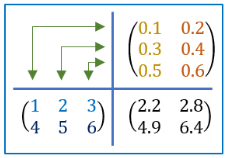
\includegraphics[width=0.8\linewidth]{matrixmultiplikation.png}
        \end{center}
        \end{minipage}
    \end{formula}
    
     \begin{theorem}{Rechenregeln für die Multiplikation von Matrizen}\\
        Assoziativ, Distributiv, nicht Kommutativ!
    \end{theorem}

    \begin{minipage}{0.65\linewidth}
        \begin{definition}{Transponierte Matrix} $A^{m \times n} \rightarrow (A^T)^{n \times m}$
            \begin{itemize}
                \item $A^T$: Spalten und Zeilen vertauscht
                \item $(A^T)_{ij} = A_{ji}$ und ${(A\cdot B)}^T = B^T\cdot A^T$
            \end{itemize}
        \end{definition}
    \end{minipage}
    \begin{minipage}{0.35\linewidth}
        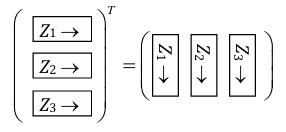
\includegraphics[width=1\linewidth]{mat-transpos.png}
    \end{minipage}

    \begin{KR}{Spezielle Matrizen}
        \begin{itemize}
            \item \textbf{Symmetrische Matrix}: $A^T = A$
            \item \textbf{Einheitsmatrix}: $E$ mit $e_{ij} = 1$ für $i = j$ und $e_{ij} = 0$ für $i \neq j$
            \item \textbf{Diagonalmatrix}: $a_{ij} = 0$ für $i \neq j$
            \item \textbf{Dreiecksmatrix}: $a_{ij} = 0$ für $i > j$ (obere Dreiecksmatrix) \\oder $i < j$ (untere Dreiecksmatrix)
        \end{itemize}
    \end{KR}

\subsubsection*{Lineare Gleichungssysteme (LGS)}
    
        \begin{definition}{Lineares Gleichungssystem (LGS)}
            Ein \textit{lineares Gleichungssystem} ist eine Sammlung von Gleichungen, 
            die linear in den Unbekannten sind. 
            Ein LGS kann in Matrixform $A\cdot\vec{x}=\vec{b}$ dargestellt werden.\\
            \begin{minipage}
                {0.45\linewidth}
                {\small
                $A$: Koeffizientenmatrix\\
                $\vec{x}$: Vektor der Unbekannten\\
                $\vec{b}$: Vektor der Konstanten}
            \end{minipage}
            \begin{minipage}{0.55\linewidth}
                $\begin{psmallmatrix} a_{11} & \cdots & a_{1n} \\ \scalebox{0.5}{\vdots} & \cdots & \scalebox{0.5}{\vdots} \\ a_{m1} & \cdots & a_{mn} \end{psmallmatrix} \cdot \begin{psmallmatrix}
                    x_1 \\ \scalebox{0.5}{\vdots} \\ x_n
                \end{psmallmatrix} = \begin{psmallmatrix}
                    b_1 \\ \scalebox{0.5}{\vdots} \\ b_m
                \end{psmallmatrix}$
            \end{minipage}
        \end{definition}

    
        \begin{theorem}{Rang einer Matrix} $rg(A)$ = Anzahl Zeilen - Anzahl Nullzeilen
            
            $\Rightarrow$ Anzahl linear unabhängiger Zeilen- oder Spaltenvektoren
        \end{theorem}


\begin{concept}{Zeilenstufenform (Gauss)}
    \begin{itemize}
        \item Alle Nullen stehen unterhalb der Diagonalen, Nullzeilen zuunterst
        \item Die erste Zahl $\neq 0$ in jeder Zeile ist eine führende Eins
        \item Führende Einsen, die weiter unten stehen $\rightarrow$ stehen weiter rechts
    \end{itemize}
    \textbf{Reduzierte Zeilenstufenform: (Gauss-Jordan)}\\
    Alle Zahlen links und rechts der führenden Einsen sind Nullen.
\end{concept}

\begin{KR}{Zeilenperationen} erlaubt bei LGS (z.B. Gauss-Verfahren)
        \begin{itemize}
            \item Vertauschen von Zeilen
            \item Multiplikation einer Zeile mit einem Skalar
            \item Addition eines Vielfachen einer Zeile zu einer anderen
        \end{itemize}
    \end{KR}
    
    \begin{formula}{Gauss-Jordan-Verfahren}
        \begin{enumerate}
            \item bestimme linkeste Spalte mit Elementen $\neq 0$ (Pivot-Spalte)
            \item oberste Zahl in Pivot-Spalte $= 0$\\ $\rightarrow$ vertausche Zeilen so dass $a_{11} \neq 0$
            \item teile erste Zeile durch $a_{11}$ $\rightarrow$ so erhalten wir führende Eins
            \item Nullen unterhalb führender Eins erzeugen (Zeilenperationen)
        \end{enumerate}
        nächste Schritte: ohne bereits bearbeitete Zeilen Schritte 1-4 wiederholen, bis Matrix Zeilenstufenform hat
    \end{formula}

    

    \begin{theorem}{Lösbarkeit von linearen Gleichungssystemen}

        \begin{minipage}{0.5\linewidth}
            \begin{itemize}
                \item Lösbar: $rg(A) = rg(A|b)$
                \item genau eine Lösung: $rg(A) = n$
            \end{itemize}
        \end{minipage}
        \begin{minipage}{0.5\linewidth}
            \begin{itemize}
                \item unendlich viele Lösungen:\\ $rg(A) < n$
            \end{itemize}
        \end{minipage}
    \end{theorem}

    \begin{KR}{Parameterdarstellung} bei unendlich vielen Lösungen

        \begin{minipage}{0.74\linewidth}
            Führende Unbekannte: Spalte mit führender Eins\\
            Freie Unbekannte: Spalten ohne führende Eins
        \end{minipage}
        \begin{minipage}{0.25\linewidth}
            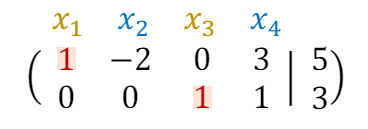
\includegraphics[width=1\linewidth]{parameterdarstellung_lgs.png}
        \end{minipage}

        \vspace{1mm}
        
        Auflösung nach der führenden Unbekannten:
        \begin{itemize}
            \item $1 x_1 - 2 x_2 + 0 x_3 + 3 x_4 = 5 \quad x_2 = \lambda \rightarrow x_1 = 5 + 2 \cdot \lambda - 3 \cdot \mu$
            \item $0 x_1 + 0 x_2 + 1 x_3 + 1 x_4 = 3 \quad x_4 = \mu \rightarrow x_3 = 3 - \mu$    
        \end{itemize}
        \vspace*{2mm}
        $$ \vec{x} = \begin{psmallmatrix} x_1 \\ x_2 \\ x_3 \\ x_4 \end{psmallmatrix} 
        = \begin{psmallmatrix} 5 + 2 \lambda - 3 \mu \\ \lambda \\ 3 - \mu \\ \mu \end{psmallmatrix} 
        = \begin{psmallmatrix} 5 \\ 0 \\ 3 \\ 0 \end{psmallmatrix} + \lambda \begin{psmallmatrix} 2 \\ 1 \\ 0 \\ 0 \end{psmallmatrix} + \mu \begin{psmallmatrix} -3 \\ 0 \\ -1 \\ 1 \end{psmallmatrix}$$
    \end{KR}

    \begin{definition}{Homogenes LGS}
        $\vec{b}=\vec{0} \rightarrow A\cdot\vec{x}=\vec{0} \rightarrow rg(A)=rg(A\mid\vec{b})$\\
        nur zwei Möglichkeiten:
            \begin{itemize}
                \item eine Lösung $x_1=x_2=\cdots=x_n=0$, die sog. \textit{triviale Lösung}.
                \item unendlich viele Lösungen
            \end{itemize}
    \end{definition}

    \begin{theorem}{Koeffizientenmatrix{,} Determinante{,} Lösbarkeit des LGS }\\
        Für $n\times n$-Matrix $A$ sind folgende Aussagen äquivalent:
    
        \vspace{1mm}
    
        \begin{minipage}{0.3\linewidth}
            \begin{itemize}
                \item $\det(A)\neq 0$
                \item $rg(A)=n$
                \item $A$ ist invertierbar
            \end{itemize}
        \end{minipage}
        \begin{minipage}{0.7\linewidth}
            \begin{itemize}
                \item Spalten von $A$ sind linear unabhängig.
                \item Zeilen von $A$ sind linear unabhängig.
                \item LGS $A\cdot\vec{x}=\vec{0}$ \\hat eindeutige Lösung $x=A^{-1}\cdot 0=0$
            \end{itemize}
        \end{minipage}
    \end{theorem}


  

\subsubsection*{Quadratische Matrizen}

\paragraph{Inverse}
    \begin{definition}{Inverse einer quadratischen Matrix A} $A^{-1}$ 
        
        $A^{-1}$ existiert, wenn $rg(A) = n$. $A^{-1}$ ist eindeutig bestimmt.

        \vspace{1mm}

        {\small Eine Matrix heisst \textit{invertierbar / regulär}, wenn sie eine Inverse hat. 
        Andernfalls heisst sie \textit{singulär}}
    \end{definition}
  
    \begin{theorem}{Eigenschaften invertierbarer Matrizen}
        \begin{itemize}
            \item $A\cdot A^{-1}=A^{-1}\cdot A=E$ und $(A^{-1})^{-1}=A$
            \item ${(A\cdot B)}^{-1}=B^{-1}\cdot A^{-1}$ {\small $\quad$ Die Reihenfolge ist relevant!}
            \item $A$ und $B$ invertierbar $\Rightarrow$ $AB$ invertierbar
            \item ${(A^T)^{-1}}={(A^{-1})}^T$ $\quad$ $A$ invertierbar $\Rightarrow$ $A^T$ invertierbar
        \end{itemize}
    \end{theorem}

\begin{theorem}{Inverse einer $2 \times 2$-Matrix} $A = \begin{psmallmatrix} a & b \\ c & d \end{psmallmatrix}$ mit $det(A) = ad - bc$
        $$A^{-1} = \frac{1}{\det(A)} \cdot \begin{pmatrix} d & -b \\ -c & a \end{pmatrix}$$
        NUR Invertierbar falls $ad - bc \neq 0$
\end{theorem}

\begin{KR}{Inverse berechnen} einer quadratischen Matrix $A^{n \times n}$
    $$A \cdot A^{-1} = E \rightarrow ( A | E ) \leadsto \text{Zeilenoperationen} \leadsto ( E | A^{-1})$$
\end{KR}

\begin{concept}{LGS mit Inverse lösen}
    $A \cdot \vec{x} = \vec{b}$
    $$A^{-1} \cdot A \cdot \vec{x} = A^{-1} \cdot \vec{b} \rightarrow \vec{x} = A^{-1} \cdot \vec{b}$$
    Beispiel:\\
    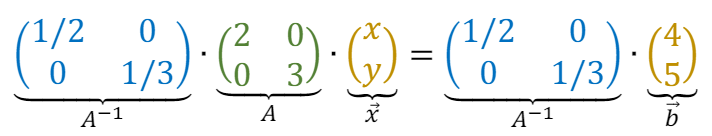
\includegraphics[width=0.7\linewidth]{lgs_inverse.png}
\end{concept}

\subsubsection{Pivotisierung}

\begin{concept}{Permutationsmatrix} $P$ ist eine Matrix, die aus der Einheitsmatrix durch Zeilenvertauschungen entsteht. 
    \vspace{1mm}\\
    \begin{minipage}[t]{0.5\textwidth}
        Für die Vertauschung der $i$-ten und $j$-ten Zeile hat $P_k$ die \textbf{Form}:
        \begin{itemize}
            \item $p_{ii} = p_{jj} = 0$ 
            \item $p_{ij} = p_{ji} = 1$
            \item Sonst gleich wie in $E_n$
        \end{itemize}
    \end{minipage}
    \hspace{3mm}
    \begin{minipage}[t]{0.45\textwidth}
        \vspace{1mm}
        \textbf{Wichtige Eigenschaften}:
        \begin{itemize}
            \item $P^{-1} = P^T = P$
            \item Mehrere Vertauschungen:\\ $P = P_l \cdot ... \cdot P_1$
        \end{itemize}
    \end{minipage}
\end{concept}

\begin{example2}{Zeilenvertauschung} für Matrix A mit Permutationsmatrix $P_1$:
    \vspace{1mm}\\
\begin{minipage}[t]{0.5\textwidth}
    $\underbrace{\begin{psmallmatrix}
    1 & 2 & 3\\
    4 & 5 & 6\\
    7 & 8 & 9
    \end{psmallmatrix}}_{A} \cdot 
    \underbrace{\begin{psmallmatrix}
    0 & 0 & 1\\
    0 & 1 & 0\\
    1 & 0 & 0
    \end{psmallmatrix}}_{P_1} =
    \begin{psmallmatrix}
    7 & 8 & 9\\
    4 & 5 & 6\\
    1 & 2 & 3
    \end{psmallmatrix}$
\end{minipage}
\begin{minipage}[t]{0.45\textwidth}
    \vspace{-2mm}
    $\Rightarrow A \cdot P_1$ bewirkt die Vertauschung von Zeile 1 und 3
\end{minipage}
\end{example2}

\vspace{-1mm}
\subsubsection{Pivotisierung}

\begin{concept}{Spaltenpivotisierung}\\
Strategie zur numerischen Stabilisierung des Gauss-Algorithmus durch Auswahl des betragsmäßig größten Elements als Pivotelement.

Vor jedem Eliminationsschritt in Spalte $i$:
\begin{itemize}
    \item Suche $k$ mit $|a_{ki}| = \max\{|a_{ji}| \mid j = i,\ldots,n\}$
    \item Falls $a_{ki} \neq 0$: Vertausche Zeilen $i$ und $k$
    \item Falls $a_{ki} = 0$: Matrix ist singulär
\end{itemize}
\end{concept}

\begin{KR}{Gauss-Algorithmus mit Pivotisierung}\\
\textbf{1. Elimination (Vorwärts)}:
\begin{itemize}
    \item Für $i=1,\ldots,n-1$:
    \begin{itemize}
    \item Finde $k \geq i$ mit $|a_{ki}| = \max\{|a_{ji}| \mid j = i,\ldots,n\}$
    \item Falls $a_{ki} = 0$: Stop (Matrix singulär)
    \item Vertausche Zeilen $i$ und $k$
    \item Für $j=i+1,\ldots,n$:
    \begin{itemize}
    \item $z_j := z_j - \frac{a_{ji}}{a_{ii}}z_i$
    \end{itemize}
    \end{itemize}
\end{itemize}
\vspace{-2mm}
\resizebox{\columnwidth}{!}{
\textbf{2. Rückwärtseinsetzen}:
$x_i = \frac{b_i - \sum_{j=i+1}^n a_{ij}x_j}{a_{ii}}, \quad i=n,n-1,\ldots,1$
}
\end{KR}

\begin{concept}{Vorteile der Permutationsmatrix}
    \begin{itemize}
        \item Exakte Nachverfolgung aller Zeilenvertauschungen
        \item Einfache Rückführung auf ursprüngliche Reihenfolge durch $P^{-1}$
        \item Kompakte Darstellung mehrerer Vertauschungen
        \item Numerisch stabile Implementierung der Pivotisierung
    \end{itemize}
\end{concept}





\section{Numerische Lösung linearer Gleichungssysteme}

\subsection{Matrix-Zerlegungen}

\begin{definition}{Dreieckszerlegung}
Eine Matrix $A \in \mathbb{R}^{n\times n}$ kann zerlegt werden in:
\vspace{1mm}\\
\begin{minipage}[t]{0.5\textwidth}
    \textbf{Untere Dreiecksmatrix L:}\\
    $l_{ij} = 0$ für $j > i$\\
    Diagonale normiert ($l_{ii}=1$)
\end{minipage}
\hspace{3mm}
\begin{minipage}[t]{0.45\textwidth}
    \textbf{Obere Dreiecksmatrix R:}\\
    $r_{ij} = 0$ für $i > j$\\
    Diagonalelemente $\neq 0$
\end{minipage}
\end{definition}


\subsubsection{LR-Zerlegung}

\begin{theorem}{LR-Zerlegung}\\
Jede reguläre Matrix $A$, für die der Gauss-Algorithmus ohne Zeilenvertauschungen durchführbar ist, lässt sich zerlegen in:
$A = LR$
wobei $L$ eine normierte untere und $R$ eine obere Dreiecksmatrix ist.
\end{theorem}

\begin{KR}{LR-Zerlegung durchführen}
    $(E | A | E) \underbrace{\leadsto}_{Gauss} (P | R | L)$
    \vspace{-3mm}\\
\begin{enumerate}
    \item Zerlegung bestimmen:
    \begin{itemize}
        \item Gauss-Elimination durchführen
        \item Eliminationsfaktoren $-\frac{a_{ji}}{a_{ii}}$ in $L$ speichern
        \item Resultierende obere Dreiecksmatrix ist $R$
    \end{itemize}
    
    \item System lösen:
    \begin{itemize}
        \item Vorwärtseinsetzen: $Ly = b$
        \item Rückwärtseinsetzen: $Rx = y$
    \end{itemize}
    
    \item Bei Pivotisierung:
    \begin{itemize}
        \item Permutationsmatrix $P$ erstellen
        \item $PA = LR$ speichern
        \item $Ly = Pb$ lösen
    \end{itemize}
\end{enumerate}
\end{KR}

\begin{remark}
    $E$ = Einheitsmatrix, $P$ = Permutationsmatrix
\end{remark}


\begin{example2}{LR-Zerlegung}
$\underbrace{\begin{psmallmatrix}
-1 & 1 & 1\\
1 & -3 & -2\\
5 & 1 & 4
\end{psmallmatrix}}_{A}, \underbrace{\begin{psmallmatrix}
0\\
5\\
3
\end{psmallmatrix}}_{b}
\rightarrow \begin{vsmallmatrix}
0 & 0 & 1\\
0 & 1 & 0\\
1 & 0 & 0
\end{vsmallmatrix} \begin{vsmallmatrix}
-1 & 1 & 1\\
1 & -3 & -2\\
5 & 1 & 4
\end{vsmallmatrix}
\begin{vsmallmatrix}
1 & 0 & 0\\
0 & 1 & 0\\
0 & 0 & 1
\end{vsmallmatrix}$

\paragraph{Schritt 1: Erste Spalte}
Max. Element in 1. Spalte: $|a_{31}| = 5$, also Z1 und Z3 tauschen:

\begin{minipage}{0.5\textwidth}
$$\begin{vsmallmatrix}
0 & 0 & 1\\
0 & 1 & 0\\
1 & 0 & 0
\end{vsmallmatrix} \begin{vsmallmatrix}
5 & 1 & 4\\
1 & -3 & -2\\
-1 & 1 & 1
\end{vsmallmatrix}
\begin{vsmallmatrix}
1 & 0 & 0\\
0 & 1 & 0\\
0 & 0 & 1
\end{vsmallmatrix}$$
\end{minipage}
\begin{minipage}{0.45\textwidth}
    \vspace{2mm}
    Eliminationsfaktoren:\\
    $l_{21} = \frac{1}{5}, \quad l_{31} = -\frac{1}{5}$
\end{minipage}


Nach Elimination:
$\begin{vsmallmatrix}
0 & 0 & 1\\
0 & 1 & 0\\
1 & 0 & 0
\end{vsmallmatrix} \begin{vsmallmatrix}
5 & 1 & 4\\
0 & -3.2 & -2.8\\
0 & 1.2 & 1.8
\end{vsmallmatrix}
\begin{vsmallmatrix}
1 & 0 & 0\\
\frac{1}{5} & 1 & 0\\
-\frac{1}{5} & 0 & 1
\end{vsmallmatrix}$

\paragraph{Schritt 2: Zweite Spalte}
Max. Element in 2. Spalte unter Diagonale: $|-3.2| > |1.2|$, \\ keine Vertauschung nötig.
Eliminationsfaktor:
$l_{32} = \frac{1.2}{-3.2} = -\frac{3}{8}$
\vspace{2mm}\\
Nach Elimination:
$\underbrace{\begin{vsmallmatrix}
0 & 0 & 1\\
0 & 1 & 0\\
1 & 0 & 0
\end{vsmallmatrix}}_{P} \underbrace{\begin{vsmallmatrix}
5 & 1 & 4\\
0 & -3.2 & -2.8\\
0 & 0 & 0.75
\end{vsmallmatrix}}_{R}
\underbrace{\begin{vsmallmatrix}
1 & 0 & 0\\
\frac{1}{5} & 1 & 0\\
-\frac{1}{5} & -\frac{3}{8} & 1
\end{vsmallmatrix}}_{L}$

\paragraph{Lösung des Systems}
\begin{enumerate}
    \item $Pb = \begin{psmallmatrix} 3\\ 5\\ 0 \end{psmallmatrix}$
    \item Löse $Ly = Pb$ durch Vorwärtseinsetzen:
    $y = \begin{psmallmatrix} 3\\ 4.4\\ 2.25 \end{psmallmatrix}$
    \item Löse $Rx = y$ durch Rückwärtseinsetzen:
    $x = \begin{psmallmatrix} -1\\ -4\\ 3 \end{psmallmatrix}$
\end{enumerate}

Probe:
$Ax = \begin{psmallmatrix}
-1 & 1 & 1\\
1 & -3 & -2\\
5 & 1 & 4
\end{psmallmatrix} \begin{psmallmatrix} -1\\ -4\\ 3 \end{psmallmatrix} = \begin{psmallmatrix} 0\\ 5\\ 3 \end{psmallmatrix} = b$
\end{example2}

\columnbreak

\subsubsection{QR-Zerlegung}

\begin{concept}{QR-Zerlegung}\\
Eine orthogonale Matrix $Q \in \mathbb{R}^{n\times n}$ erfüllt: $Q^T Q = QQ^T = I_n$
\vspace{1mm}\\
Die QR-Zerlegung einer Matrix $A$ ist: $A = QR$
\vspace{1mm}\\
wobei $Q$ orthogonal und $R$ eine obere Dreiecksmatrix ist.
\end{concept}

\begin{definition}{Householder-Transformation}\\
Eine Householder-Matrix hat die Form:
$H = I_n - 2uu^T$

mit $u \in \mathbb{R}^n$, $\|u\| = 1$. Es gilt:
\begin{itemize}
    \item $H$ ist orthogonal ($H^T = H^{-1}$) und symmetrisch ($H^T = H$)
    \item $H^2 = I_n$
\end{itemize}
\end{definition}

\begin{KR}{QR-Zerlegung mit Householder}
\begin{enumerate}
    \item Initialisierung: $R := A$, $Q := I_n$
    \item Für $i = 1,\ldots,n-1$:
        \begin{itemize}
            \item Bilde Vektor $v_i$ aus i-ter Spalte von $R$ ab Position $i$
            \item $w_i := v_i + \text{sign}(v_{i1})\|v_i\|e_1$
            \item $u_i := w_i/\|w_i\|$
            \item $H_i := I_{n-i+1} - 2u_iu_i^T$
            \item Erweitere $H_i$ zu $Q_i$ durch $I_{i-1}$ links oben
            \item $R := Q_iR$ und $Q := QQ_i^T$
        \end{itemize}
\end{enumerate}
\end{KR}

\begin{example2}[breakable]{QR-Zerlegung mit Householder}
    %TODO: check if this is correct and/or relevant - either correct or replace with better example
$A = \begin{psmallmatrix}
2 & 5 & -1\\
-1 & -4 & 2\\
0 & 2 & 1
\end{psmallmatrix}$

\paragraph{Schritt 1: Erste Spalte}
Erste Spalte $a_1$ und Einheitsvektor $e_1$:
$a_1 = \begin{psmallmatrix} 2\\ -1\\ 0 \end{psmallmatrix}, \quad e_1 = \begin{psmallmatrix} 1\\ 0\\ 0 \end{psmallmatrix}$

Householder-Vektor für erste Spalte:
\vspace{1mm}
\begin{enumerate}
    \item Berechne Norm: $|a_1| = \sqrt{2^2 + (-1)^2 + 0^2} = \sqrt{5}$
    \vspace{1mm}
    \item Bestimme Vorzeichen: $\text{sign}(a_{11}) = \text{sign}(2) = 1$
         \begin{itemize}
              \item Wähle positives Vorzeichen, da erstes Element positiv
              \item Dies maximiert die erste Komponente von $v_1$
              \item Verhindert Auslöschung bei der Subtraktion
         \end{itemize}
         \vspace{1mm}
    \item $v_1 = a_1 + \text{sign}(a_{11})|a_1|e_1 = \begin{psmallmatrix} 2\\ -1\\ 0 \end{psmallmatrix} + \sqrt{5}\begin{psmallmatrix} 1\\ 0\\ 0 \end{psmallmatrix} = \begin{psmallmatrix} 2 + \sqrt{5}\\ -1\\ 0 \end{psmallmatrix}$
    \vspace{1mm}
    \item Normiere $v_1$: $|v_1| = \sqrt{(2 + \sqrt{5})^2 + 1} \Rightarrow
            u_1 = \frac{v_1}{|v_1|} = \begin{psmallmatrix} 0.91\\ -0.41\\ 0 \end{psmallmatrix}$
\end{enumerate}
\vspace{1mm}
Householder-Matrix berechnen:
$H_1 = I - 2u_1u_1^T = \begin{psmallmatrix} 
-0.67 & -0.75 & 0\\
-0.75 & 0.67 & 0\\
0 & 0 & 1
\end{psmallmatrix}$
A nach 1. Transformation:
$A^{(1)} = H_1A = \begin{psmallmatrix}
-\sqrt{5} & -6.71 & 0.45\\
0 & -0.89 & 1.79\\
0 & 2.00 & 1.00
\end{psmallmatrix}$
\paragraph{Schritt 2: Zweite Spalte}
Untermatrix für zweite Transformation:
$A_2 = \begin{psmallmatrix} -0.89 & 1.79\\ 2.00 & 1.00 \end{psmallmatrix}$

Householder-Vektor für zweite Spalte:
\vspace{1mm}
\begin{enumerate}
    \item $|a_2| = \sqrt{(-0.89)^2 + 2^2} = 2.19$
    \vspace{1mm}
    \item $\text{sign}(a_{22}) = \text{sign}(-0.89) = -1$ (da erstes Element negativ)
    \vspace{1mm}
    \item $v_2 = \begin{psmallmatrix} -0.89\\ 2.00 \end{psmallmatrix} - 2.19\begin{psmallmatrix} 1\\ 0 \end{psmallmatrix} = \begin{psmallmatrix} -3.09\\ 2.00 \end{psmallmatrix}$
    \vspace{1mm}
    \item $u_2 = \frac{v_2}{|v_2|} = \begin{psmallmatrix} -0.84\\ 0.54 \end{psmallmatrix}$
\end{enumerate}
\vspace{1mm}
Erweiterte Householder-Matrix: %TODO: nicer formatting!
$Q_2 = \begin{psmallmatrix}
1 & 0 & 0\\
0 & -0.41 & -0.91\\
0 & -0.91 & 0.41
\end{psmallmatrix}$

nach 2. Transformation:
$R = Q_2A^{(1)} = \begin{psmallmatrix}
-\sqrt{5} & -6.71 & 0.45\\
0 & -2.19 & 1.34\\
0 & 0 & -1.79
\end{psmallmatrix}$

\paragraph{Endergebnis}
Die QR-Zerlegung $A = QR$ ist:

$Q = H_1^TQ_2^T = \begin{psmallmatrix}
-0.89 & -0.45 & 0\\
0.45 & -0.89 & 0\\
0 & 0 & 1
\end{psmallmatrix},
R = \begin{psmallmatrix}
-\sqrt{5} & -6.71 & 0.45\\
0 & -2.19 & 1.34\\
0 & 0 & -1.79
\end{psmallmatrix}$

\paragraph{Probe}
\small
\begin{enumerate}
    \item $QR = A$ (bis auf Rundungsfehler)
    \item $Q^TQ = QQ^T = I$ (Orthogonalität)
    \item $R$ ist obere Dreiecksmatrix
\end{enumerate}

\paragraph{Wichtige Beobachtungen}
\small
\begin{itemize}
    \item Vorzeichenwahl bei $v_k$ ist entscheidend für numerische Stabilität
    \item Ein falsches Vorzeichen kann zu Auslöschung führen
    \item Betrag der Diagonalelemente in $R$ = Norm transformierter Spalten
    \item $Q$ ist orthogonal: Spaltenvektoren sind orthonormal
\end{itemize}
\end{example2}




\subsubsection{Iterative Verfahren}

\begin{definition}{Zerlegung der Systemmatrix} $A$ zerlegt in: $A = L + D + R$
    \small
\begin{itemize}
    \item $L$: streng untere Dreiecksmatrix
    \item $D$: Diagonalmatrix
    \item $R$: streng obere Dreiecksmatrix
\end{itemize}
\end{definition}

\begin{concept}{Jacobi-Verfahren}
Gesamtschrittverfahren 
\vspace{1mm}\\
Iteration: $x^{(k+1)} = -D^{-1}(L + R)x^{(k)} + D^{-1}b$
\vspace{1mm}\\
Komponentenweise:
$x_i^{(k+1)} = \frac{1}{a_{ii}}(b_i - \sum_{j=1,j\neq i}^n a_{ij}x_j^{(k)})$
\end{concept}

\begin{concept}{Gauss-Seidel-Verfahren}
Einzelschrittverfahren 
\vspace{1mm}\\
Iteration: $x^{(k+1)} = -(D+L)^{-1}Rx^{(k)} + (D+L)^{-1}b$
\vspace{1mm}\\
Komponentenweise:\\
$x_i^{(k+1)} = \frac{1}{a_{ii}}(b_i - \sum_{j=1}^{i-1} a_{ij}x_j^{(k+1)} - \sum_{j=i+1}^n a_{ij}x_j^{(k)})$
\end{concept}

\begin{theorem}{Konvergenzkriterien}
Ein iteratives Verfahren konvergiert, wenn:
\begin{enumerate}
    \item Die Matrix $A$ diagonaldominant ist:\\
    $|a_{ii}| > \sum_{j\neq i} |a_{ij}|$ für alle $i$
    \item Der Spektralradius der Iterationsmatrix kleiner 1 ist:\\
    $\rho(B) < 1$ mit $B$ als jeweilige Iterationsmatrix
\end{enumerate}
\end{theorem}

\begin{KR}{Implementierung von Jacobi- und Gauss-Seidel-Verfahren}
    \paragraph{Vorbereitungsphase}
    \begin{itemize}
        \item Matrix zerlegen in $A = L + D + R$
        \item Diagonaldominanz prüfen: $|a_{ii}| > \sum_{j\neq i} |a_{ij}|$ für alle $i$
        \item Sinnvolle Startwerte wählen (z.B. $x^{(0)}=0$ oder $x^{(0)}=b$)
        \item Toleranz $\epsilon$ und max. Iterationszahl $n_{max}$ festlegen
    \end{itemize}

    \paragraph{Verfahren durchführen}
    \begin{itemize}
        \item \textbf{Jacobi}: Komponentenweise parallel berechnen 
        \item \textbf{Gauss-Seidel}: Komponentenweise sequentiell berechnen 
    \end{itemize}

    \paragraph{Konvergenzprüfung/Abbruchkriterien}
    \begin{itemize}
        \item Absolute Änderung: $\|x^{(k+1)} - x^{(k)}\| < \epsilon$
        \item Relatives Residuum: $\frac{\|Ax^{(k)} - b\|}{\|b\|} < \epsilon$
        \item Maximale Iterationszahl: $k < n_{max}$
    \end{itemize}

    \paragraph{A-priori Fehlerabschätzung}
    \begin{itemize}
        \item Spektralradius $\rho$ der Iterationsmatrix bestimmen
        \item Benötigte Iterationen $n$ für Genauigkeit $\epsilon$:\\
        $n \geq \frac{\ln(\epsilon(1-\rho)/\|x^{(1)}-x^{(0)}\|)}{\ln(\rho)}$
    \end{itemize}
\end{KR}







\subsubsection{Fehleranalyse}

\begin{definition}{Matrix- und Vektornormen}\\
Eine Vektornorm $\|\cdot\|$ erfüllt für alle $x,y \in \mathbb{R}^n, \lambda \in \mathbb{R}$:
\begin{itemize}
    \item $\|x\| \geq 0$ und $\|x\| = 0 \Leftrightarrow x = 0$
    \item $\|\lambda x\| = |\lambda| \cdot \|x\|$
    \item $\|x + y\| \leq \|x\| + \|y\|$ (Dreiecksungleichung)
\end{itemize}
\end{definition}

\begin{concept}{Wichtige Normen}

\textbf{1-Norm:}
        $\|x\|_1 = \sum_{i=1}^n |x_i|,
        \|A\|_1 = \max_j \sum_{i=1}^n |a_{ij}|$

\textbf{2-Norm:}
        $\|x\|_2 = \sqrt{\sum_{i=1}^n x_i^2}, 
        \|A\|_2 = \sqrt{\rho(A^TA)}$

$\infty$\textbf{-Norm:}
        $\|x\|_\infty = \max_i |x_i|, 
        \|A\|_\infty = \max_i \sum_{j=1}^n |a_{ij}|$
\end{concept}

\begin{theorem}{Fehlerabschätzung für LGS}\\
Sei $\|\cdot\|$ eine Norm, $A \in \mathbb{R}^{n\times n}$ regulär und $Ax = b$, $A\tilde{x} = \tilde{b}$
\vspace{1mm}\\
\begin{minipage}[t]{0.47\textwidth}
    \textbf{Absoluter Fehler:}
    \vspace{-5mm}\\
    \begin{center}
        $\|x - \tilde{x}\| \leq \|A^{-1}\| \cdot \|b - \tilde{b}\|$
    \end{center}
\end{minipage}
\hspace{2mm}
\begin{minipage}[t]{0.47\textwidth}
    \textbf{Relativer Fehler:}
    \vspace{-5mm}\\
    \begin{center}
        $\frac{\|x - \tilde{x}\|}{\|x\|} \leq \text{cond}(A) \cdot \frac{\|b - \tilde{b}\|}{\|b\|}$
    \end{center}
\end{minipage}
\vspace{1mm}\\
Mit der Konditionszahl $\text{cond}(A) = \|A\| \cdot \|A^{-1}\|$
\end{theorem}

\begin{concept}{Konditionierung}\\
Die Konditionszahl beschreibt die numerische Stabilität eines LGS:
\begin{itemize}
    \item $\text{cond}(A) \approx 1$: gut konditioniert
    \item $\text{cond}(A) \gg 1$: schlecht konditioniert
    \item $\text{cond}(A) \to \infty$: singulär
\end{itemize}
\end{concept}

\begin{example2}{Konditionierung}
$A = \begin{psmallmatrix}
1 & 1\\
1 & 1.01
\end{psmallmatrix}, b = \begin{psmallmatrix}
2\\
2.01
\end{psmallmatrix}$\\
Konditionszahl:
$\text{cond}(A) = \|A\| \cdot \|A^{-1}\| \approx 400$
\paragraph{Fehlerabschätzung}
$\text{Absoluter Fehler: }\|x - \tilde{x}\| \leq 400 \cdot 0.01 = 4$ \\
$\text{Relativer Fehler: }\frac{\|x - \tilde{x}\|}{\|x\|} \leq 400 \cdot \frac{0.01}{2} = 2$
\end{example2}

\begin{KR}{Vergleich Lösungsverfahren}
$A = \begin{psmallmatrix}
1 & 2 & 0\\
2 & 1 & 2\\
0 & 2 & 1
\end{psmallmatrix}, \quad b = \begin{psmallmatrix}
1\\
2\\
3
\end{psmallmatrix}$

\small
\begin{itemize}
    \item Matrix ist symmetrisch und nicht streng diagonaldominant
    \item $\text{cond}_\infty(A) \approx 12.5$
\end{itemize}
\begin{center}
\begin{tabular}{l|ccc}
Verfahren & Iterationen & Residuum & Zeit\\
\hline
LR mit Pivot & 1 & $2.2\cdot10^{-16}$ & 1.0\\
QR & 1 & $2.2\cdot10^{-16}$ & 2.3\\
Jacobi & 12 & $1.0\cdot10^{-6}$ & 1.8\\
Gauss-Seidel & 7 & $1.0\cdot10^{-6}$ & 1.4\\
\end{tabular}
\end{center}
\vspace{-2mm}
\begin{itemize}
    \item Direkte Verfahren erreichen höhere Genauigkeit
    \item Iterative Verfahren brauchen mehrere Schritte
\end{itemize}
\end{KR}

\begin{example2}{Konvergenzverhalten}
$\begin{psmallmatrix}
4 & 1 & 0\\
1 & 4 & 1\\
0 & 1 & 4
\end{psmallmatrix}
\begin{psmallmatrix}
x_1\\
x_2\\
x_3
\end{psmallmatrix} =
\begin{psmallmatrix}
1\\
2\\
3
\end{psmallmatrix}$
\vspace{1mm}\\
\small
Die Matrix ist diagonaldominant:
$|a_{ii}| = 4 > 1 = \sum_{j\neq i} |a_{ij}|$
\vspace{1mm}\\
\begin{tabular}{c|cc|cc}
k & \multicolumn{2}{c|}{Residuum} & \multicolumn{2}{c}{Rel. Fehler}\\
& Jacobi & G-S & Jacobi & G-S\\
\hline
0 & 3.74 & 3.74 & - & -\\
1 & 0.94 & 0.47 & 0.935 & 0.468\\
2 & 0.23 & 0.06 & 0.246 & 0.125\\
3 & 0.06 & 0.01 & 0.065 & 0.017\\
4 & 0.01 & 0.001 & 0.016 & 0.002
\end{tabular}

\paragraph{Beobachtungen:}
\begin{itemize}
    \item Gauss-Seidel konvergiert etwa doppelt so schnell wie Jacobi
    \item Das Residuum fällt linear (geometrische Folge)
    \item Die Konvergenz ist gleichmäßig (keine Oszillationen)
\end{itemize}
\end{example2}

\subsubsection{Vorgehen und Implementation}

\begin{KR}{Systematisches Vorgehen bei LGS}
\begin{enumerate}
    \item Eigenschaften der Matrix analysieren:
    \begin{itemize}
        \item Diagonaldominanz prüfen
        \item Konditionszahl berechnen oder abschätzen
        \item Symmetrie erkennen
    \end{itemize}
    
    \item Verfahren auswählen:
    \begin{itemize}
        \item Direkte Verfahren: für kleinere Systeme
        \item Iterative Verfahren: für große, dünnbesetzte Systeme
        \item Spezialverfahren: für symmetrische/bandförmige Matrizen
    \end{itemize}
    
    \item Implementation planen:
    \begin{itemize}
        \item Pivotisierung bei Gauss berücksichtigen
        \item Speicherbedarf beachten
        \item Abbruchkriterien festlegen
    \end{itemize}
\end{enumerate}
\end{KR}

\begin{KR}{Zeilenvertauschungen verfolgen}
\begin{enumerate}
    \item Initialisiere $P = I_n$
    \item Für jede Vertauschung von Zeile $i$ und $j$:
    \begin{itemize}
        \item Erstelle $P_k$ durch Vertauschen von Zeilen $i,j$ in $I_n$
        \item Aktualisiere $P = P_k \cdot P$
        \item Wende Vertauschung auf Matrix an: $A := P_kA$
    \end{itemize}
    \item Bei der LR-Zerlegung mit Pivotisierung:
    \begin{itemize}
        \item $PA = LR$ 
        \item Löse $Ly = Pb$ und $Rx = y$
    \end{itemize}
\end{enumerate}
\end{KR}



























    \raggedcolumns
    \pagebreak
    
\subsubsection{Approximations- und Rundungsfehler}

\begin{definition}{Fehlerarten}
Sei $\tilde{x}$ eine Näherung des exakten Wertes $x$:
\vspace{1mm}\\
\begin{minipage}[t]{0.45\textwidth}
    \textbf{Absoluter Fehler:} 
    \begin{center} $\left|\tilde{x}-x\right|$ \end{center}
\end{minipage}
\hspace{3mm}
\begin{minipage}[t]{0.5\textwidth}
    \textbf{Relativer Fehler:} 
    \begin{center} $\left|\frac{\tilde{x}-x}{x}\right| \text{ bzw. } \frac{|\tilde{x}-x|}{|x|} \text{ für } x \neq 0$ \end{center}
\end{minipage}
\end{definition}

\begin{concept}{Konditionierung}
    Die Konditionszahl $K$ beschreibt die relative Fehlervergrösserung bei Funktionsauswertungen:
    \vspace{1mm}\\
\begin{minipage}{0.3\textwidth}
    \vspace{-2mm}
    $$K := \frac{|f'(x)| \cdot |x|}{|f(x)|}$$
\end{minipage}
\hspace{2mm}
\begin{minipage}{0.6\textwidth}
\begin{itemize}
    \item $K \leq 1$: gut konditioniert
    \item $K > 1$: schlecht konditioniert
    \item $K \gg 1$: sehr schlecht konditioniert
\end{itemize}
\end{minipage}
\end{concept}


\begin{theorem}{Fehlerfortpflanzung}
Für $f$ (differenzierbar) gilt näherungsweise:
\vspace{1mm}\\
\begin{minipage}[t]{0.47\textwidth}
    \textbf{Absoluter Fehler:}  
    \vspace{-2mm}\\
    $$|f(\tilde{x})-f(x)| \approx |f'(x)| \cdot |\tilde{x}-x|$$
\end{minipage}
\hspace{3mm}
\begin{minipage}[t]{0.43\textwidth}
    \textbf{Relativer Fehler:}  
    \vspace{-2mm}\\
    $$\frac{|f(\tilde{x})-f(x)|}{|f(x)|} \approx K \cdot \frac{|\tilde{x}-x|}{|x|}$$
\end{minipage}
\end{theorem}



\raggedcolumns




\begin{KR}{Fehlerabschätzung für Nullstellen}\\
So schätzen Sie den Fehler einer Näherungslösung ab:
\begin{enumerate}
    \item Sei $x_n$ der aktuelle Näherungswert
    \item Wähle Toleranz $\epsilon > 0$
    \item Prüfe Vorzeichenwechsel: $f(x_n-\epsilon) \cdot f(x_n+\epsilon) < 0$
    \item Falls ja: Nullstelle liegt in $(x_n-\epsilon, x_n+\epsilon)$
    \item Damit gilt: $|x_n-\xi| < \epsilon$
\end{enumerate}
\end{KR}





















    \raggedcolumns
    \end{comment}
\end{multicols}
\end{document}